\chapter{Experimental Results}
\label{chap:experiment}
In this chapter we introduce the evaluation metrics and dataset adopted in our work firstly. Then the experiment results are shown and analyzed in detail. We also compare our model with other advanced works.

\section{Dataset}

In this study, we made use of the Database of Evoked Emotions by Speech (DEMoS)~\cite{parada2020demos}, an Italian corpus of emotional speech. The DEMoS was collected from 68 speakers (23 females and 45 males), with a total of 9,365 emotional samples and 332 neutral speech samples. Neutral speech samples were not considered in our study because neutrality is a minority class. 9,365 speech samples were annotated with the seven categories of emotion shown in Table 1, all of which were used in our experiments. Emotions in DEMoS are induced by arousal potentiation processes~\cite{parada2020demos}. To avoid speaker dependence during training, the data (training, development, and test) were partitioned independently of the speaker, taking into account a balance of affective categories. The distribution of data in the three partitions is shown in Table~\ref{table:database}.
\begin{table}[]
	\centering
	\begin{tabular}{l|llll}
		\hline
		\#        & Train & Dev  & Test & Sum  \\ \hline
		Speakers  & 27    & 21   & 20   & 68   \\ \hline
		Anger     & 603   & 451  & 423  & 1477 \\
		Disgust   & 684   & 520  & 474  & 1678 \\
		Fear      & 480   & 350  & 326  & 1156 \\
		Guilt     & 468   & 339  & 322  & 1129 \\
		Happiness & 569   & 427  & 399  & 1395 \\
		Sadness   & 640   & 455  & 435  & 1530 \\
		Surprise  & 403   & 308  & 289  & 1000 \\
		Sum       & 3847  & 2850 & 2668 & 9365
	\end{tabular}
	\caption{Speaker independent partitions, Train, (Dev)elopment, Test created from DEMoS, including the distribution of the 7-classes .}
	\label{table:database}
\end{table}

\subsection{Pre-processing Of Data}
As we found the use of log-Mel spectrogram images extracted from audio waves to be successful in the previous work~\cite{ren2018attention}, we make use of log-Mel spectrogram images as input of the deep models in this study.  First, the speech files were resampled from 44.1 kHz to 16 kHz, since 16 kHz data can lead to faster progress and data from both sampling rates had similar results in earlier experiments~\cite{9054087}. Then, we extracted log-Mel spectrogram images with a window size of 512 units, an overlap length of 256 units, and 64 mel bins. To unify the time length of log-Mel spectrogram images, we broadcast the spectrogram images with shorter time length than the longest spectrogram, resulting in a set of log-Mel spectrogram images of size (373, 64). In addition, the log-Mel spectrogram images are used as the input to the defense (CNN) model.The generated images are as follows:
\begin{figure}[!hbtp]
	\centering
	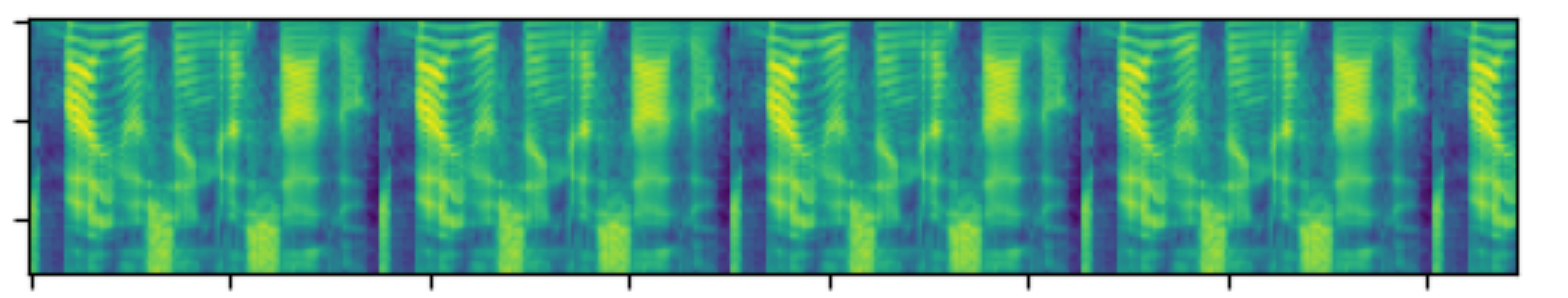
\includegraphics[width=0.9\linewidth]{figures_ning/mel-1}
	\caption[log-Mel spectrogram]{log-Mel spectrogram}
	\label{fig:mel-1}
\end{figure}

For parameter optimization during our experiments, we train the defense model on the training set and test it on the development set; the defense model used to validate the test set is trained from the combined training and development sets.Herein, three CNN architectures are employed due to CNN models' strong capability to extract high-level features from log-Mel spectrogram images~\cite{zhao2018data}. The implemented CNN models contain a conventional CNN model with four convolutional layers (named as CNN-4), a ResNet model, and a VGG model.
The CNN-4 model contains, four convolutional layers $[64,128,256,512]$, a global max pooling layer, a fully connected layer, and a softmax layer for the final classification. The four convulutional layers have a kernel with a size of $(5, 5)$, and each convulutional layer is followed by a local max pooling layer with a kernel size of $(2, 2)$. The global max pooling has shown better performance than flattening in our previous study~\cite{ren2018attention}, as it can extract smaller feature vectors from feature maps for classification.
Besides the CNN-4 model, another two state-of-the-art CNN models, ResNet and VGG, are employed for a comparison. ResNet~\cite{szegedy2017inception} contains the Inception architecture which requires relatively low computational cost. ResNet has shown promise in the tasks of image processing~\cite{szegedy2017inception}. ResNet has a series of structures with different numbers of layers. One of them, ResNet-50 ~\cite{he2016deep}, is utilised, since our work is focusing on adversarial attacks and training. Moreover, VGG has shown good performance on processing spectrogram images for audio classification tasks due to its deep architecture~\cite{simonyan2015very,ren2018learning}. Hence, we also train a VGG-16 model for this speech-based emotion recognition task.

\begin{table}[]
	\centering
	\begin{tabular}{c|c}
		\hline
		\#        & Probability    \\ \hline
		CNN-4     & surprise:0.995 \\ \hline
		VGG-16    & surprise:0.988 \\
		ResNet-50 & surprise:0.997
	\end{tabular}
	\caption[label of log-Mel spectrogram]{label of log-Mel spectrogram}
\end{table}

\section{Evaluation Metrics}
When training the black-box attack model in this study, the attacker does not know the parameters of the target model. The input data is first fed to the attack model to generate fake data, similar to the original input data (Figure 1(a)). The target model (i.e., the defense) is then unable to generate correct predictions for the generated data.
Regarding the inputs, log-Mel spectrograms are used due to their powerful performance in \textbf{SER}~\cite{ren2020generating,zhang2017speech} tasks. The real log-Mel spectrogram and labels are represented as $(x, y)$ and the generated adversarial data is$x^{\prime}$. The CNN model can then be trained to output a two-dimensional adversarial perturbation η. Finally, the adversarial data is obtained by $x^{\prime}=x+\eta$. Due to the ability to output features, an atrous CNN model is proposed to generate mappings with adversarial perturbations of the same size as the input~\cite{ren2019attention}. Efficient training of aerobic
CNN attack model, the loss function has two objectives: one is to deceive the defense $f$, and the other is to minimize the difference between fake and real data. Thus, the loss function is a weighted sum of the loss functions of the two objectives:
$$
\begin{gathered}
	\operatorname{loss}=\operatorname{\alpha oss}_{\text {cla }}\left(f\left(\boldsymbol{x}^{\prime}\right)\right)+(1-\alpha) \operatorname{loss}_{M S E}\left(\boldsymbol{x}^{\prime}, \boldsymbol{x}\right) \\
	\operatorname{loss}_{c l a}\left(f\left(x^{\prime}\right)\right)=\max \left(f\left(x^{\prime}\right)_{l}-\max \left(f\left(x^{\prime}\right)_{\text {other }}\right), 0\right)
\end{gathered}
$$

where $\alpha$ is the hyperparameter that balances the two loss functions $\operatorname{loss}_{c l a}$ and $\operatorname{loss}_{M S E}$. The loss function $\operatorname{loss}_{c l a}$ aims to reduce the defensive classification performance on false data, and $\operatorname{loss}_{M S E}$ aims to improve the similarity between false and true data using mean square error (MSE). The function losscla is defined by the difference between the probability of the correct label l and the maximum probability of the other classes. The calculation of losscla is known as the Carlini-Wagner $(\mathrm{C} \& \mathrm{~W})$ loss function~\cite{bose2018adversarial}. This approach has been used to generate adversarial attacks in image processing tasks~\cite{akhtar2018threat,bose2018adversarial}.
The log-Mel spectrogram after the attack model is as follows:
\begin{figure}[!hbtp]
	\centering
	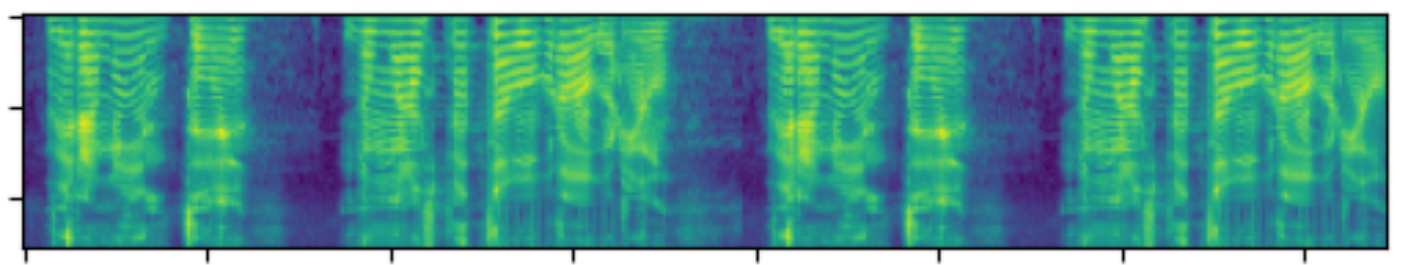
\includegraphics[width=0.9\linewidth]{figures_ning/mel-2}
	\caption[Fake log-Mel spectrogram]{Fake log-Mel spectrogram}
	\label{fig:mel-2}
\end{figure}

\begin{figure}[!hbtp]
	\centering
	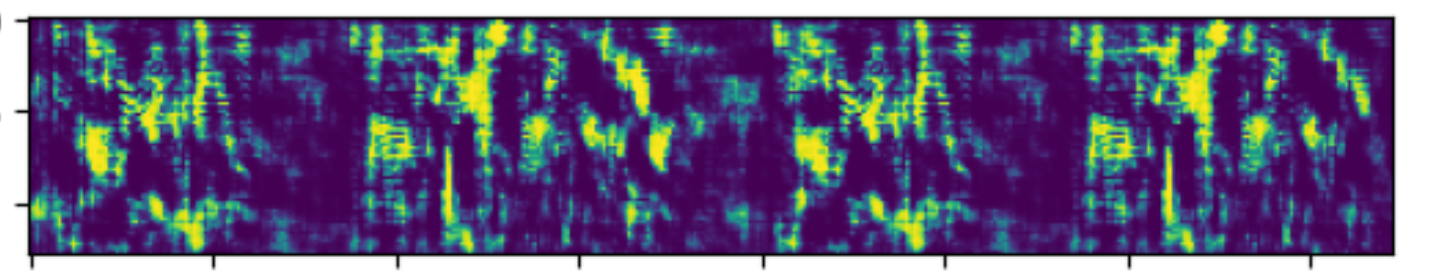
\includegraphics[width=0.9\linewidth]{figures_ning/mel-3}
	\caption[Adversarial perturbation]{Adversarial perturbation}
	\label{fig:mel-3}
\end{figure}

\begin{figure}[!hbtp]
	\centering
	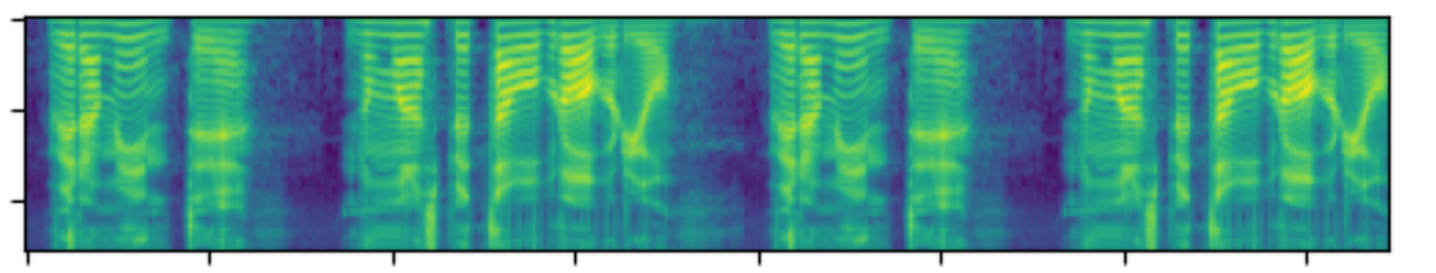
\includegraphics[width=0.9\linewidth]{figures_ning/mel-4}
	\caption[Real log-Mel spectrogram]{Real log-Mel spectrogram}
	\label{fig:mel-4}
\end{figure}

After that we use the changed spectrogram as input and re-judged by the three defense models to obtain the following results:
\begin{table}[!h]
	\centering
	\begin{tabular}{c|c|c}
		\#        & Probability of Real log-Mel spectrogram & Probability of Fake log-Mel spectrogram \\ \hline
		CNN-4     & Surprise:0.995                          & Guilt:0.586                             \\
		VGG-16    & Surprise:0.988                          & Anger:0.878                             \\
		ResNet-50 & Surprise:0.997                          & Anger:0.788                            
	\end{tabular}
	\caption[Classification of log Mel spectrogram]{Classification of log Mel spectrogram}
	\label{tab:log-2}
\end{table}

This proves the success of the attack. The original audio message(log-Mel spectrogram) was classified as Surprise, and after the attack model we designed, it became Guilt or Anger. we don't care about the specific category of the final classification, as long as it doesn't match the original label, it shows the success of our black box attack.

For the presentation of the final experimental results, the Unweighted Average Recall (UAR), which is an unweighted average result, is used as an evaluation metric considering the category imbalance. This is because the classifier of the defense model has seven labels, but each label corresponds to a different number of audio files. Our purpose is to judge the accuracy of each emotion, and if we directly use all the number of labels to judge the accuracy, it will produce a large error. For example, if the data is divided unevenly, there are 3847 messages in the training set, among which there are 2000 Angry labels, so that the proportion of Angry labels is much higher than 1/7. If our attack model has good aggressiveness for angry audio messages, if the final accuracy obtained by the defense model is only 0.100, but the aggressiveness for other audio messages is poorer If we use the average accuracy directly, the result is 0.302, as in Table~\ref{tab:dir}; however, if we use UAR calculation, as in Table 2, the result is 0.461~\ref{tab:uar}. 
\begin{table}[!hbtp]
	\centering
	\subtable[Directly Average Accuracy]{
		\begin{tabular}{l|ll}
			\centering
			Scene Label   & Number & Accuracy \\ \hline
			Anger         & 2000   & 0.100    \\
			Other Emotion & 1847   & 0.521    \\
			Sum           & 3847   & 0.302   
			\label{tab:dir}
	\end{tabular}}
	\subtable[Unweighted Average Recall]{
		\begin{tabular}{l|ll}
			Scene Label   & Number & Accuracy \\ \hline
			Anger         & 2000   & 0.100    \\
			Other Emotion & 1847   & 0.521    \\
			Sum           & 3847   & 0.461   
			\label{tab:uar}
	\end{tabular}}
	\caption{Different Result}
	\label{tab:diff}
\end{table}

The difference between the two is very large. Such a result can only show that the attack model has obvious effect on specific audio files, but we are judging seven kinds of tags, and obviously UAR is suitable as a judgment criterion.
The following table is an example of UAR as a judgment criterion, first finding the accuracy rate of each tag, and then finding the average of the seven labels:
\begin{table}[!hbtp]
	\centering
	\begin{tabular}{l|ll}
		Scene Label & Number & Accuracy \\ \hline
		Anger       & 431    & 0.752    \\
		Disgust     & 487    & 0.827    \\
		Fear        & 643    & 0.766    \\
		Guilt       & 721    & 0.737    \\
		Happiness   & 274    & 0.817    \\
		Sadness     & 523    & 0.705    \\
		Surprise    & 768    & 0.847    \\ \hline
		Average     & 3847   & 0.779   
	\end{tabular}
	\caption{Unweighted Average Recall Of CNN-4}
	\label{tab:UAR}
\end{table}


\label{sec:experimentpixel}
\section{Experiments on Dynamic Neural Networks}
In Section~\ref{sec:pixel_base}, we put forward related ideas, through the attention map in Fig.~\ref{fig:method1baseline} to find possible relationships in the detected pictures. We hope that the most relevant area can be directly reflected in the attention map, so we designed an attention loss function(see Eq.~\ref{pixel_attention_loss}) so that the attention weights of the relevant area are higher than the non-relevant area.

We tried to add a multi-head self-attention module after obtaining the image feature in VGG16 based on the code of RelDN~\cite{zhang2019graphical},  so that we obtained a new image feature with a size of $ [bs, 512, 50, 66]  $and an  attention map with a size of $ [bs, 3300, 3300] $, where bs is batch size=2. We build the baseline as the Fig.~\ref{fig:method1baseline} shown.

\subsubsection{Result of the Pixel Attention Loss  Function}
Figure~\ref{fig:singlepixelmap} shows the attention map of a single pixel after loss function processing. The attention weights between each pixels of subject and the entire image is computed, which can be expressed as $ \forall Attention_{p^k_{sbj} \to p^i_{img}} , p^i_{img} \in \mathbb{P}_{img} $, where k is the $ k^{th} $ pixel of the subject.

\begin{figure}[h!]
	\centering
	\subfigure[$ <arm, on, man> $]{
		\begin{minipage}[t]{3.5cm}
			\centering
			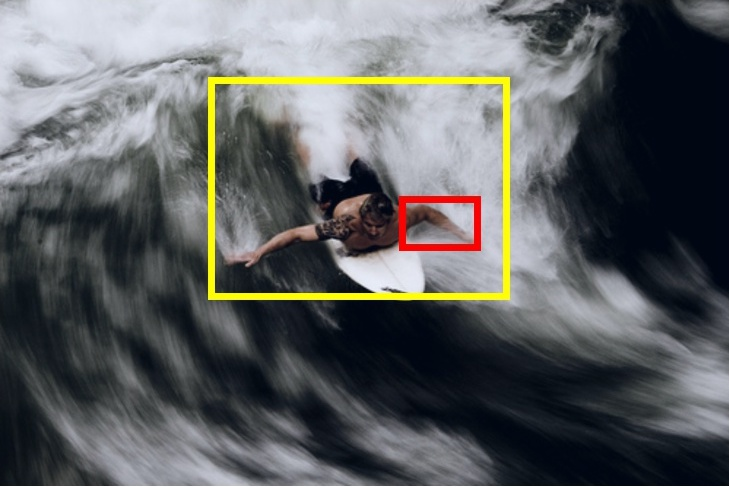
\includegraphics[width=0.9\linewidth]{figures/pixel/img2}
		\end{minipage}
		\begin{minipage}[t]{3.5cm}
			\centering
			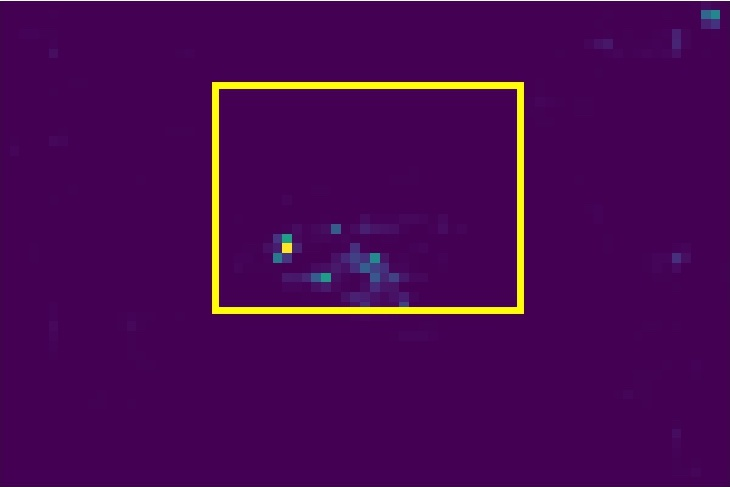
\includegraphics[width=0.9\linewidth]{figures/pixel/map2_1}
		\end{minipage}
		\begin{minipage}[t]{3.5cm}
			\centering
			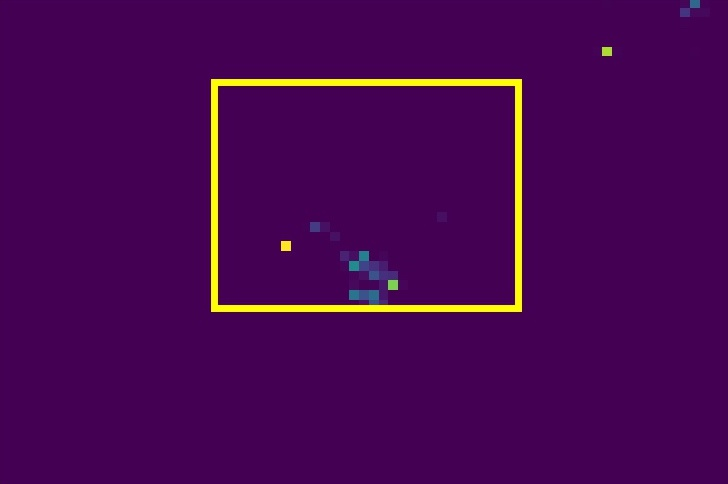
\includegraphics[width=0.9\linewidth]{figures/pixel/map2_2}
		\end{minipage}
		\begin{minipage}[t]{3.5cm}
			\centering
			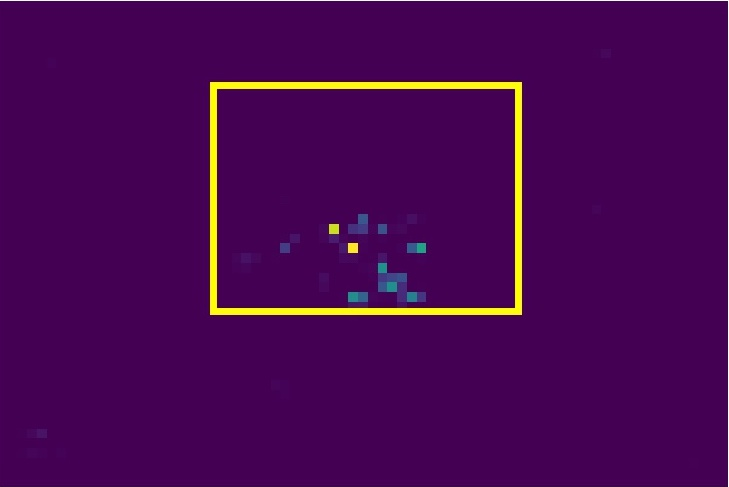
\includegraphics[width=0.9\linewidth]{figures/pixel/map2_3}
		\end{minipage}
		\label{fig:singlepixelmap_a}}
	
	\subfigure[$ <bike, has, wheel> $]{
		\begin{minipage}[t]{3.5cm}
			\centering
			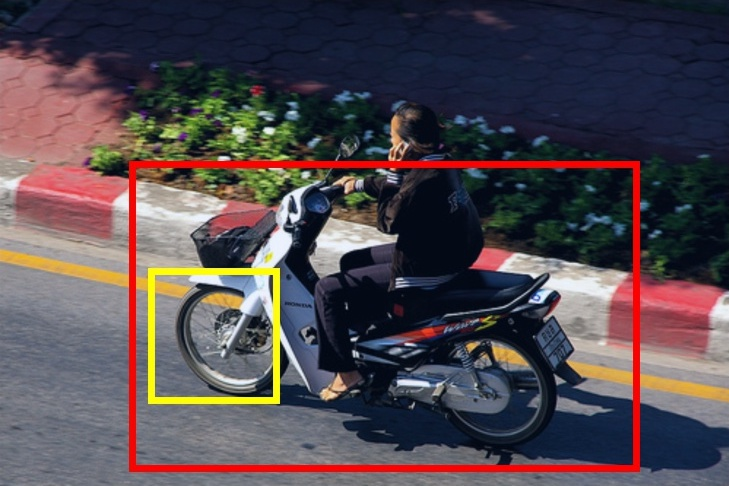
\includegraphics[width=0.9\linewidth]{figures/pixel/img3}
		\end{minipage}
		\begin{minipage}[t]{3.5cm}
			\centering
			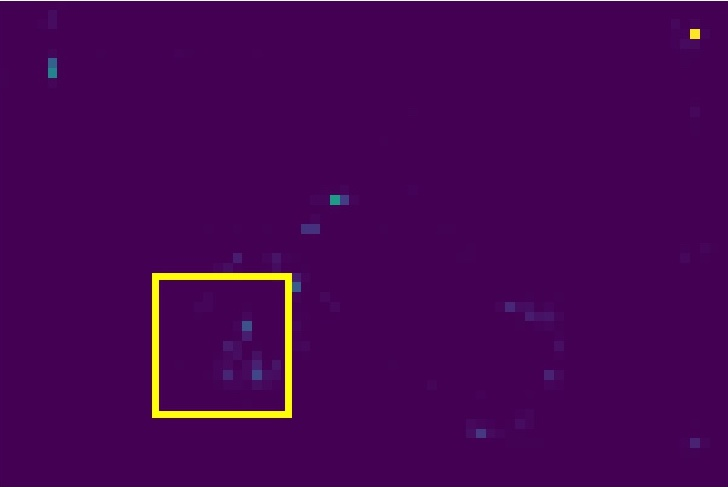
\includegraphics[width=0.9\linewidth]{figures/pixel/map3_1}
		\end{minipage}
		\begin{minipage}[t]{3.5cm}
			\centering
			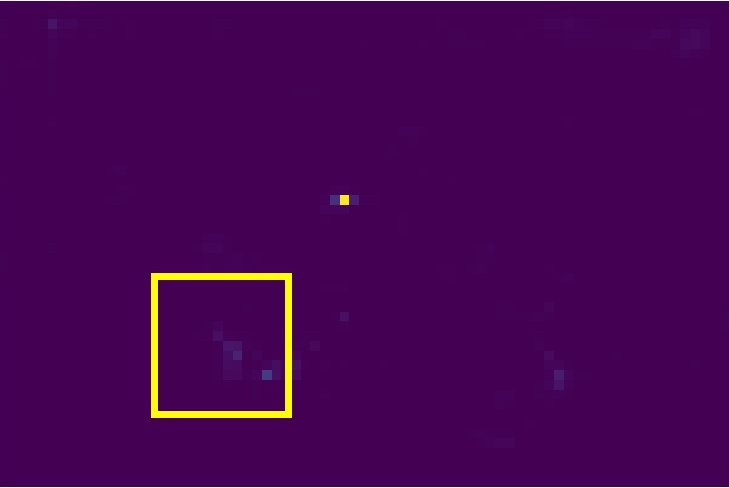
\includegraphics[width=0.9\linewidth]{figures/pixel/map3_2}
		\end{minipage}
		\begin{minipage}[t]{3.5cm}
			\centering
			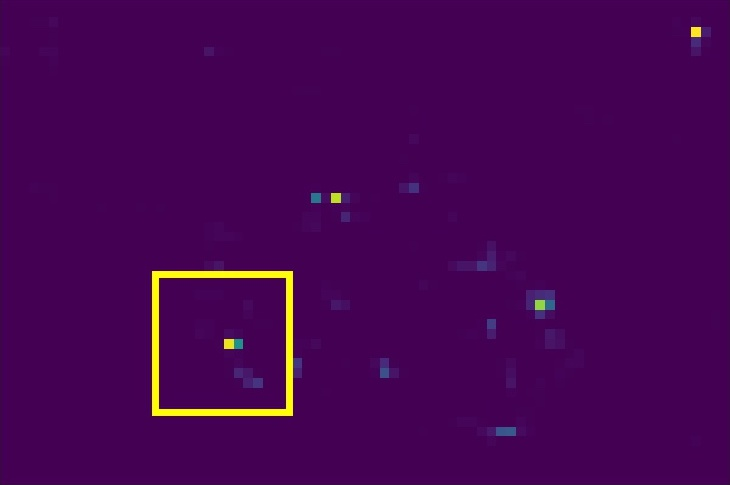
\includegraphics[width=0.9\linewidth]{figures/pixel/map3_3}
		\end{minipage}
		\label{fig:singlepixelmap_b}}
	
	
	\subfigure[$<window, on, door>$]{
		\begin{minipage}[t]{3.5cm}
			\centering
			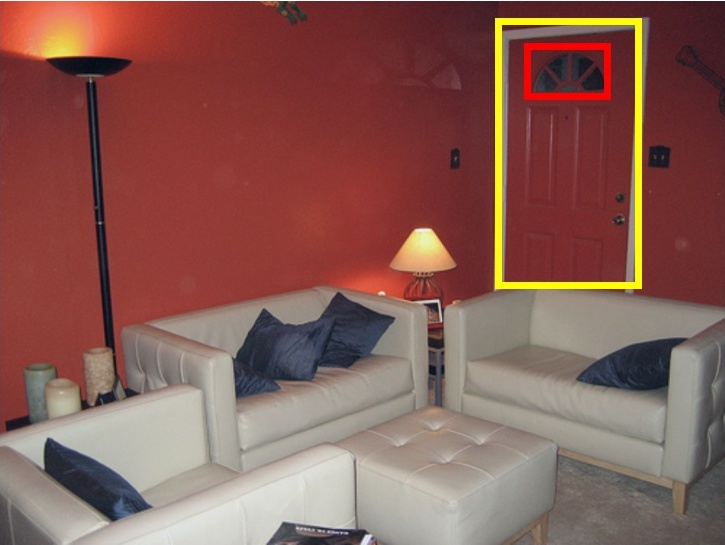
\includegraphics[width=0.9\linewidth]{figures/pixel/img4}
		\end{minipage}
		\begin{minipage}[t]{3.5cm}
			\centering
			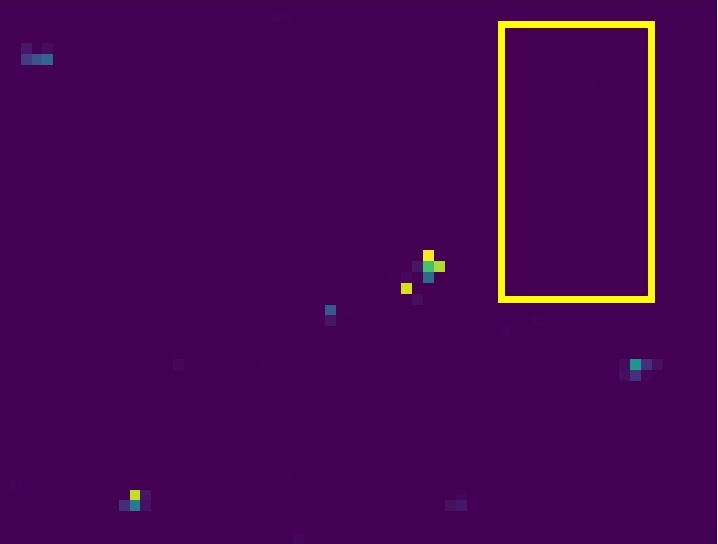
\includegraphics[width=0.9\linewidth]{figures/pixel/map4_1}
		\end{minipage}
		\begin{minipage}[t]{3.5cm}
			\centering
			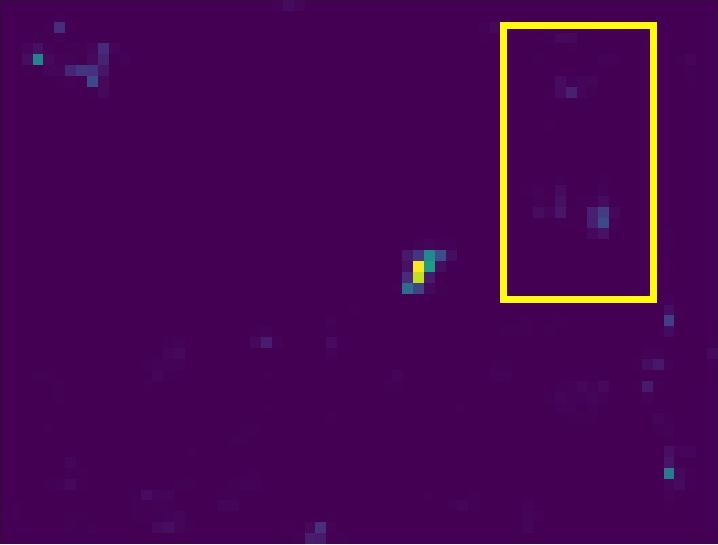
\includegraphics[width=0.9\linewidth]{figures/pixel/map4_2}
		\end{minipage}
		\begin{minipage}[t]{3.5cm}
			\centering
			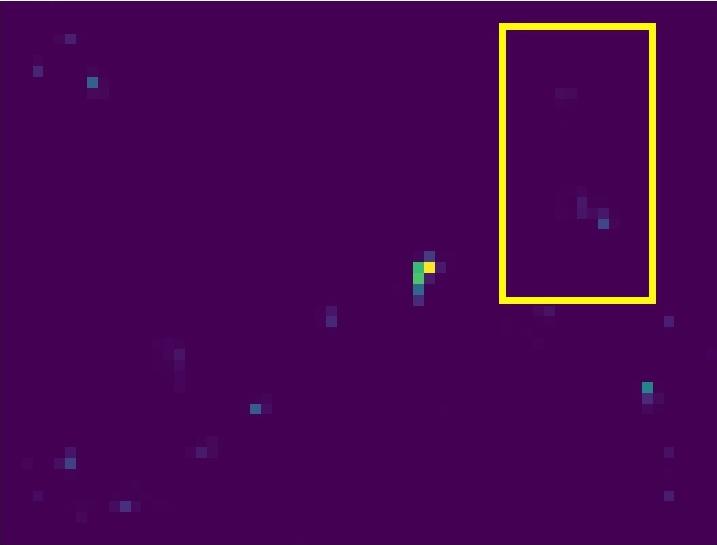
\includegraphics[width=0.9\linewidth]{figures/pixel/map4_3}
		\end{minipage}
		\label{fig:singlepixelmap_c}}
	
	\subfigure[ $<zebra, has, leg>$]{
		\begin{minipage}[t]{3.5cm}
			\centering
			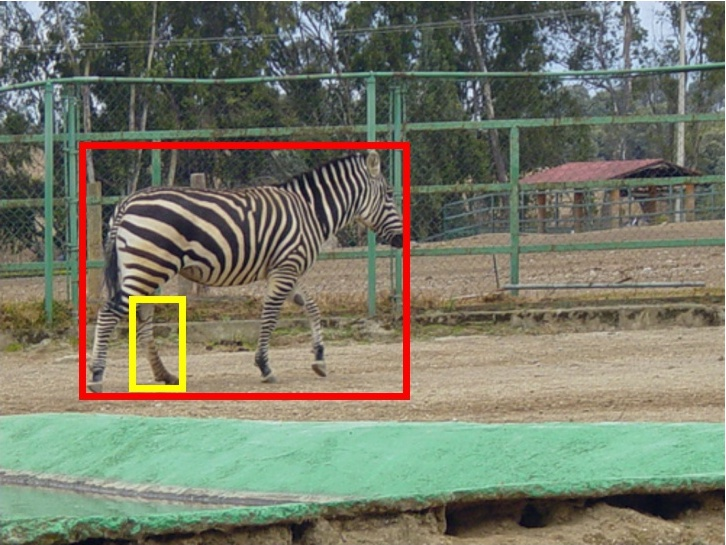
\includegraphics[width=0.9\linewidth]{figures/pixel/img5}
		\end{minipage}
		\begin{minipage}[t]{3.5cm}
			\centering
			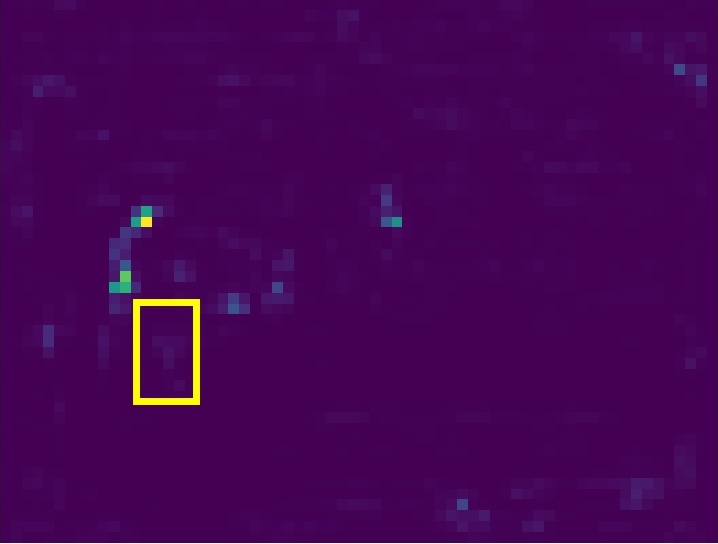
\includegraphics[width=0.9\linewidth]{figures/pixel/map5_1}
		\end{minipage}
		\begin{minipage}[t]{3.5cm}
			\centering
			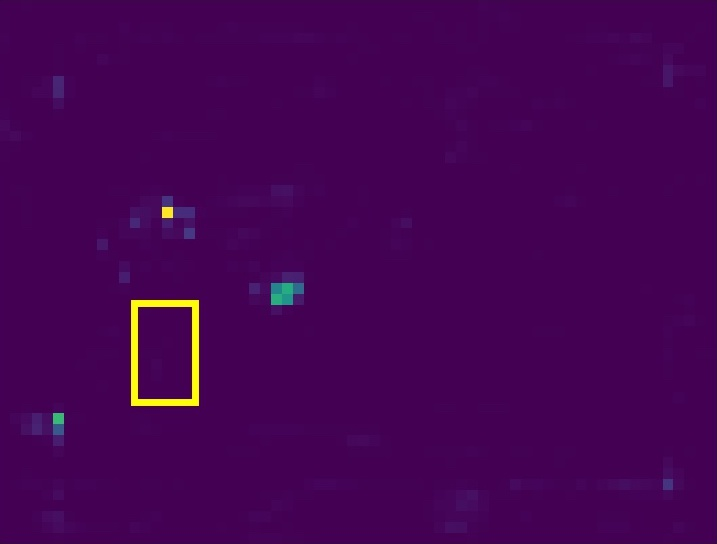
\includegraphics[width=0.9\linewidth]{figures/pixel/map5_2}
		\end{minipage}
		\begin{minipage}[t]{3.5cm}
			\centering
			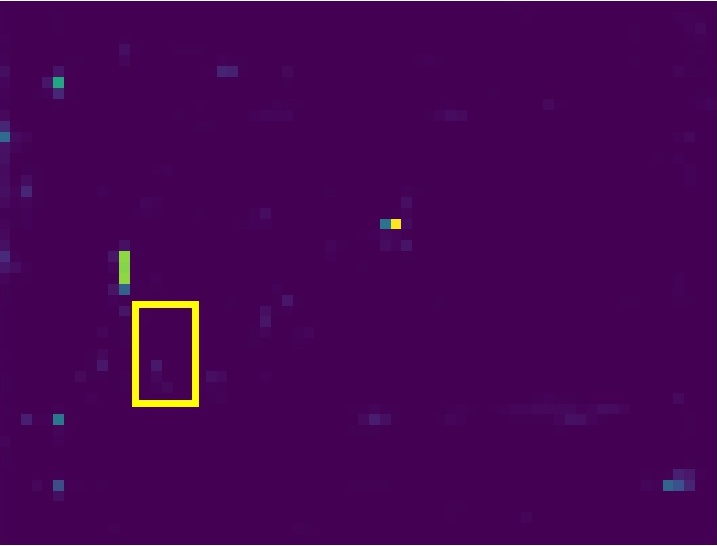
\includegraphics[width=0.9\linewidth]{figures/pixel/map5_3}
		\end{minipage}
		\label{fig:singlepixelmap_d}}
	
	\caption[Visualized results of the attention map of a single pixel ]{Visualized results of the attention map of a single pixel. The red box in the figure is subject, and the yellow box is object. We randomly select a few pixels from the subject, then draw the attention map of these pixels to the entire picture. }
	\label{fig:singlepixelmap}
\end{figure}

As shown in Figure~\ref{fig:singlepixelmap_a}, we randomly select three pixels from subject \textit{arm} and drew their attention weights map for the entire image, the red box is the subject \textit{arm} and the yellow box is the object\textit{ man}, and the ground truth relation is \textit{arm on man}. In the picture, the most highlights are in the yellow box, which means that these pixels of the subject focus more on the object \textit{man}. Although the loss function performs well in Figure (a), it works not well with the other picture, such as the Figure (b), (c), (d).

In Figure~\ref{fig:singlepixelmap_b}, the subject is \textit{bike}, and the object is \textit{wheel}. We also select three pixels from the subject and draw their attention maps. In the three attention maps, most of the highlights are out of the yellow box, which means that the pixels of subject \textit{bike} pays little attention the object \textit{wheel}, and from the distribution of the highlights it can be find that the pixels pay more attention to the rest part of the subject \textit{bike}.

In Figure~\ref{fig:singlepixelmap_c}, the subject is \textit{window}, and the object is \textit{door}. In the attention maps, the pixels of  \textit{window} pay nor attention to the subject or the object. They focus on the lamps, which has no relation with the subject \textit{window}.

The attention maps of Figure~\ref{fig:singlepixelmap_d} shows that some pixels of subject \textit{zebra} focus on the subject and some of them focus on the parts of the image except the subject and object.

After analyzing the result of the experiments, it comes to a conclusion that this loss function performs not well. With this loss function, most $ \forall Att_i^{rel} $ are not able to reflect the relation between subjects and objects. The results show that most of subjects can not pay attention to the right objects, they focus more on themselves or the parts that has no relation to them.



\begin{figure}[!h]
	\centering
	\subfigure[Image input.]{
		\begin{minipage}[t]{7.5cm}
			\centering
			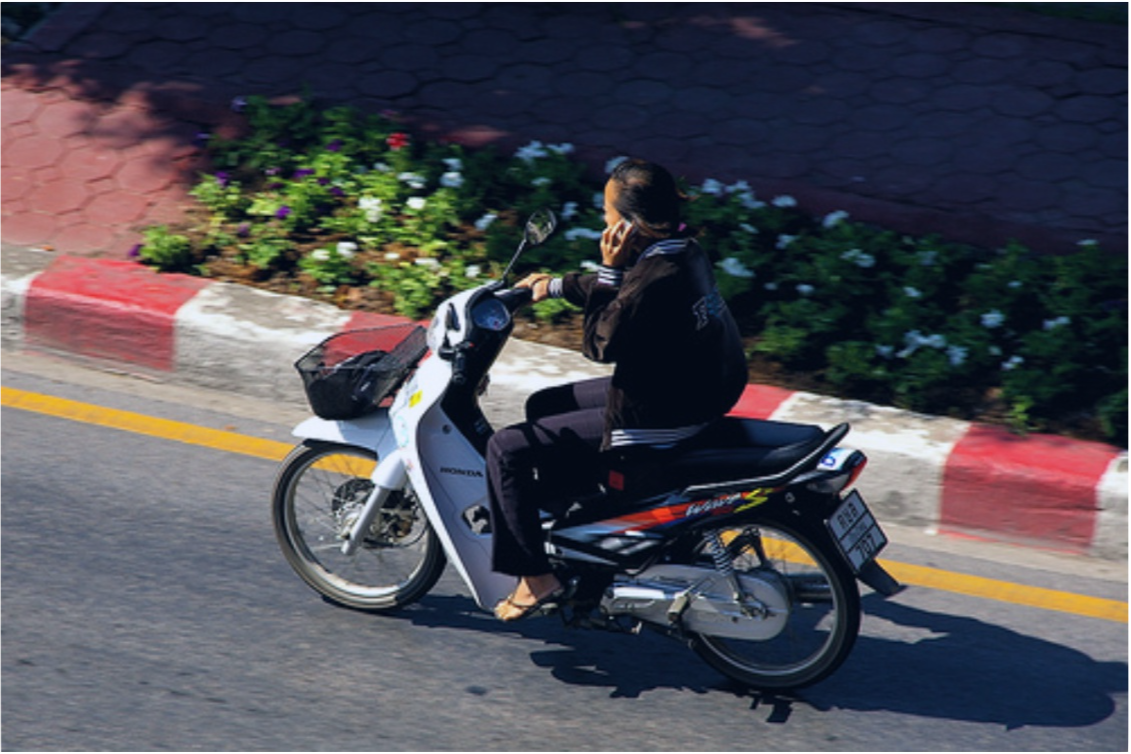
\includegraphics[width=0.95\linewidth]{figures/motor/img}
			\label{fig:motor_img}
	\end{minipage}}
	\subfigure[The result of a normalized attention map.]{
		\begin{minipage}[t]{7.5cm}
			\centering
			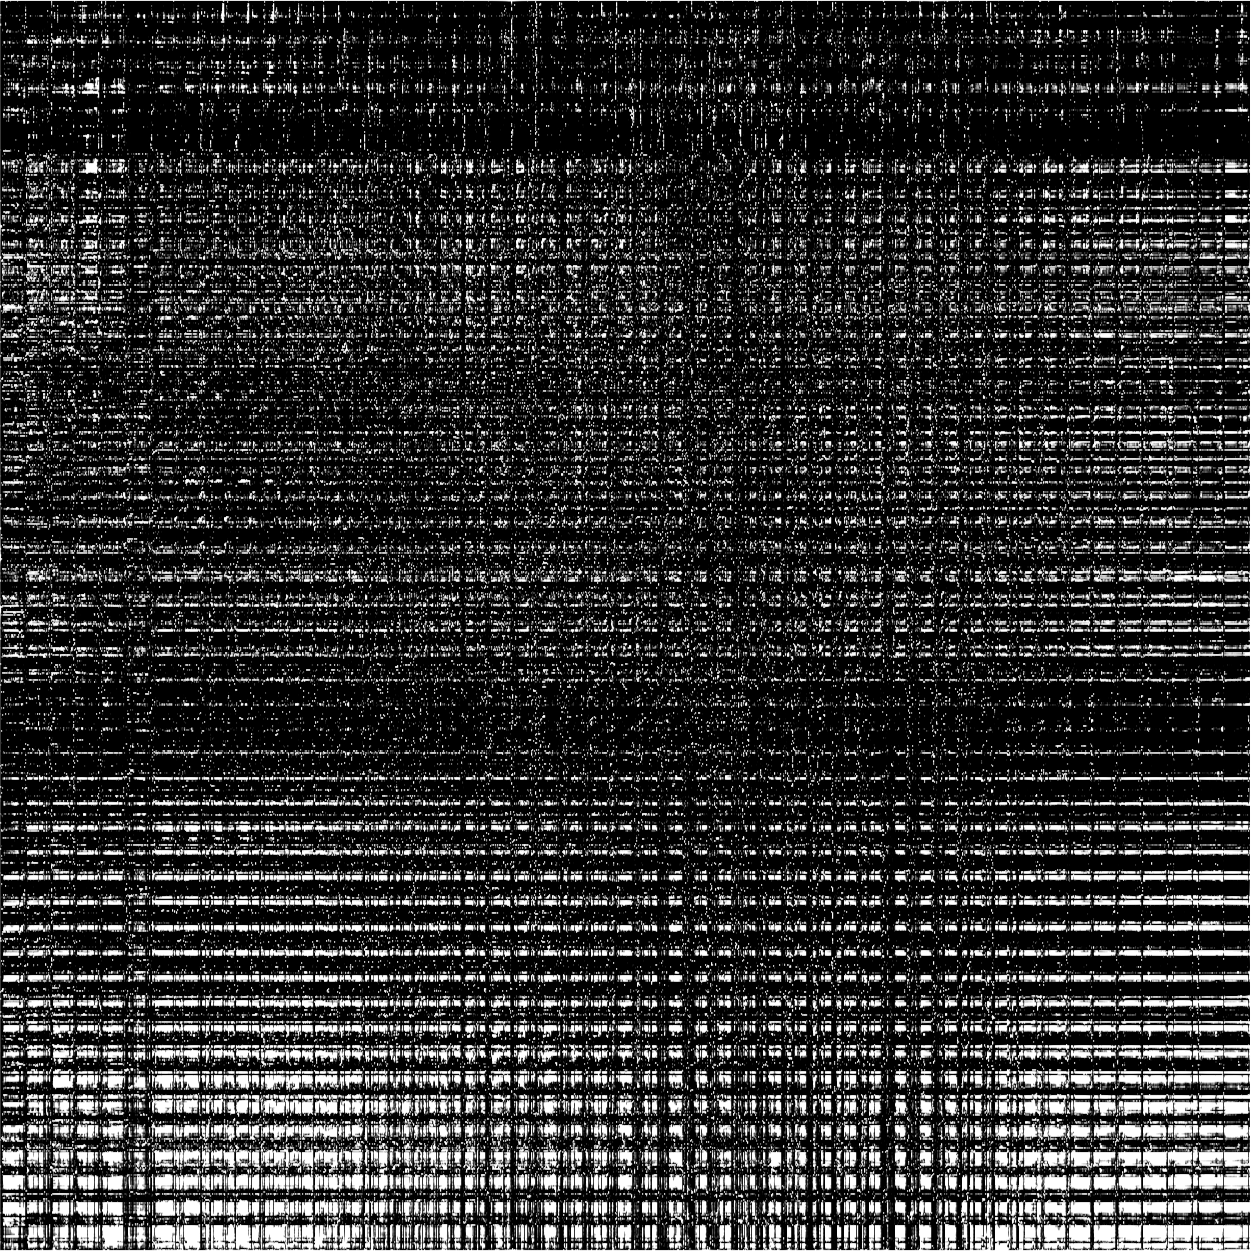
\includegraphics[width=0.8\linewidth]{figures/motor/attention}
			\label{fig:motor_attention_map}
	\end{minipage}}
	
	\caption[The result of a normalized attention map drawn by matlab]{The result of a normalized Attention Map drawn by matlab.}
	\label{fig:motor_attention}
\end{figure}

\subsubsection{Result analysis}

In order to find the cause of the above problem, the complete attention map of the Fig.~\ref{fig:motor_img} is drawn in Figure~\ref{fig:motor_attention_map}. It can be seen from the figure that the overall distribution of $ \forall Attention_{p^i_{img} \to p^j_{img}} , p^i_{img},p^j_{img} \in \mathbb{P}_{img} $ is still relatively uniform, and it is not intuitive to distinguish which objects have a relationship. It can only indicate that the loss function has changed the attention map, but this change has no benefits to the relationship detection.

Then Figure~\ref{fig:motor_pair}  shows the position about the attention weights set for each relation pair. Figure(d) shows the position of $ \forall Attention_{p^i_{man} \to p^j_{bike}} $ ,  $ \forall Attention_{p^i_{man} \to p^j_{bike}} \in \forall Att_{rel} $ in the attention map. Because the whole bike is the ground truth object, the loss function should increase its attention weights. While the white areas in Figure(e) and Figure (f) belong to $ \forall Att_{no\_rel} $, which means that the man and wheels have no intersection in this scene, the loss function should lower its attention weights.

 In Figure~\ref{fig:motor_pair}(a)(b)(c), the subject is \textit{man} and the objects are \textit{bike}, \textit{$ wheel_1 $}, \textit{$ wheel_2 $}, \textit{$ wheel_1 $} and \textit{$ wheel_2 $} belong to \textit{bike}, and there is overlap between bike and wheels. It causes that the sets of attention weights for these three relation pairs also have overlap, so this loss function cannot highlight the attention weights of $ \forall Attention_{p^i_{man} \to p^j_{bike}} $ while reducing the attention weights of  $ \forall Att_{no\_rel} $.

This overlap is so serious and in Figure~\ref{fig:overlap} there is an example analyze.The white area in Figure~\ref{fig:overlap}(a) is the position of set of all relation pairs$ Att_{rel} $  about the image in the attention map, and the white area in Figure~\ref{fig:overlap}(b)  are position of the set of all no relation pairs $ Att_{no\_rel} $.When we calculate the overlap between $Att_{rel} $ and  $Att_{no\_rel} $, we can find that the white area of Figure(b) is contained in the white area of Figure(a). It can be expressed as  $$ \forall Att^i_{rel} \cap  \forall Att^i_{no\_rel } = \forall Att^i_{rel}  $$ or $$ \forall Att^i_{rel}  \subseteq  \forall Att^i_{no\_rel }$$.

This  overlap is not a special case, almost all pictures have this problem, so the pixel attention loss becomes meaningless. It cannot make the attention weights of the overlapping areas higher or lower so the idea of pixel-based attention can not go further, and it is not feasible to use the attention between pixels to obtain which relation pair is most likely to have a relationship.

%From the results, our attention loss has made certain modifications to the attention map. But in general, the values in the attention map are relatively average, and there is no strong distinguish ability. For instance, the ground truth pair $ <man, motorcycle>  $ shown in Fig.~\ref{fig:motor_man0}, its location of the corresponding area in attention map shown in Fig.~\ref{fig:motor_map0}. We can see the attention values in the area of the attention map(Fig.~\ref{fig:motor_attention_map}) is not higher than other areas, even be low.
%
%In general, we use our  average of attention weights  of each pair to replace the original pair score ($ score_{pair}=score_{subject }*score_{predicate}* score_{object} $) in the evaluation to sort relation pairs, and it does not improve the recall rate of the relation.
%
%Then we analyzed the results, and we drew the position of all $ Att_{rel} $s and all $ Att_{no\_rel} $s in the attention map of image~\ref{fig:motor_img} , see Fig.~\ref{fig:overlap} $ (a) $ and $ (b) $ in the figure. And the overlap between them is shown in Figure $ (c). $ We found that $ Att_{rel }$ and $ Att_{no\_rel} $ have a very serious overlap, and are basically the same as $ Att_{rel }$, that is,  $ Att_{no\_rel} $ contains $ Att_{rel }$. The purpose of our Attention Loss is to make $ Att_{rel }$ higher and $ Att_{no\_rel }$ lower. The existence of this overlap makes its purpose very contradictory. For example, the area in Figure~\ref{fig:motor_all0} belongs to $ Att_{rel }$ but it also belongs to $ Att_{no\_rel }$ in Figure~\ref{fig:motor_all1}. We cannot make it higher and lower. This overlap in the image is shown in Figure~\ref{fig:motor_pair}. For example, for the same subject $ man $, there are  pairs $<man,ride,motorcycle>$, $ <man, \varnothing, wheel_1> $  and  $ <man, \varnothing, wheel_2>  $, their objects have an overlap, and the bounding box  of $ motor $ obviously contains the bounding box of  $ wheel $.
%
%This overlap is not a special case. We found that almost all images have this situation, so the attention loss we designed is meaningless, and the idea of Piexl-based Attention also failed. We cannot use the attention between pixels to obtain which pair is most likely to have a relationship.

\begin{figure}[h!]
	\centering
	\subfigure[$<man,ride,bike>$]{
		\begin{minipage}[t]{5cm}
			\centering
			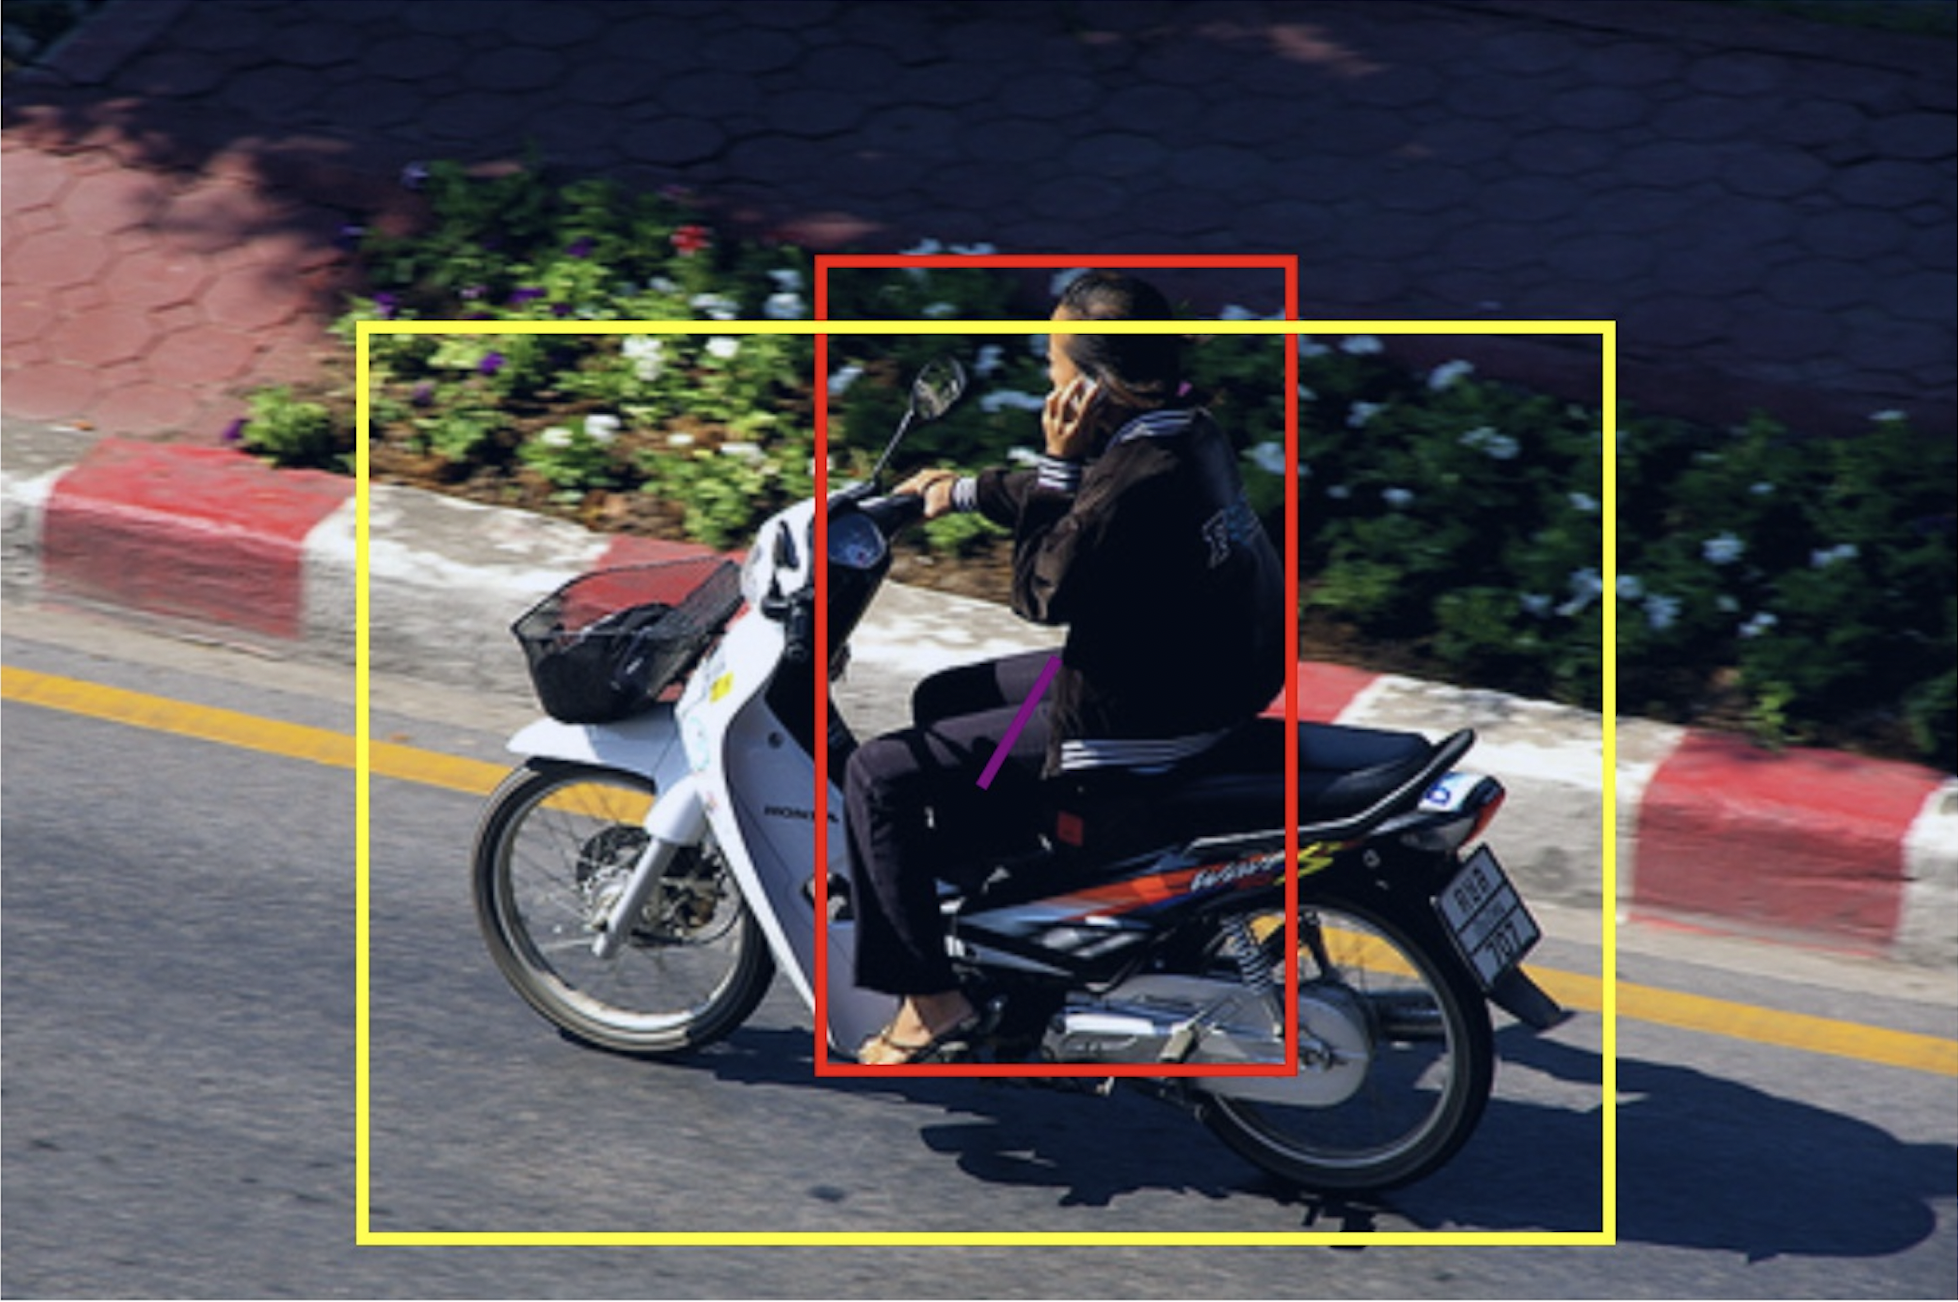
\includegraphics[width=0.9\linewidth]{figures/motor/man0}
			\label{fig:motor_man0}
	\end{minipage}}
	\subfigure[$ <man, \varnothing, wheel_1> $]{
		\begin{minipage}[t]{5cm}
			\centering
			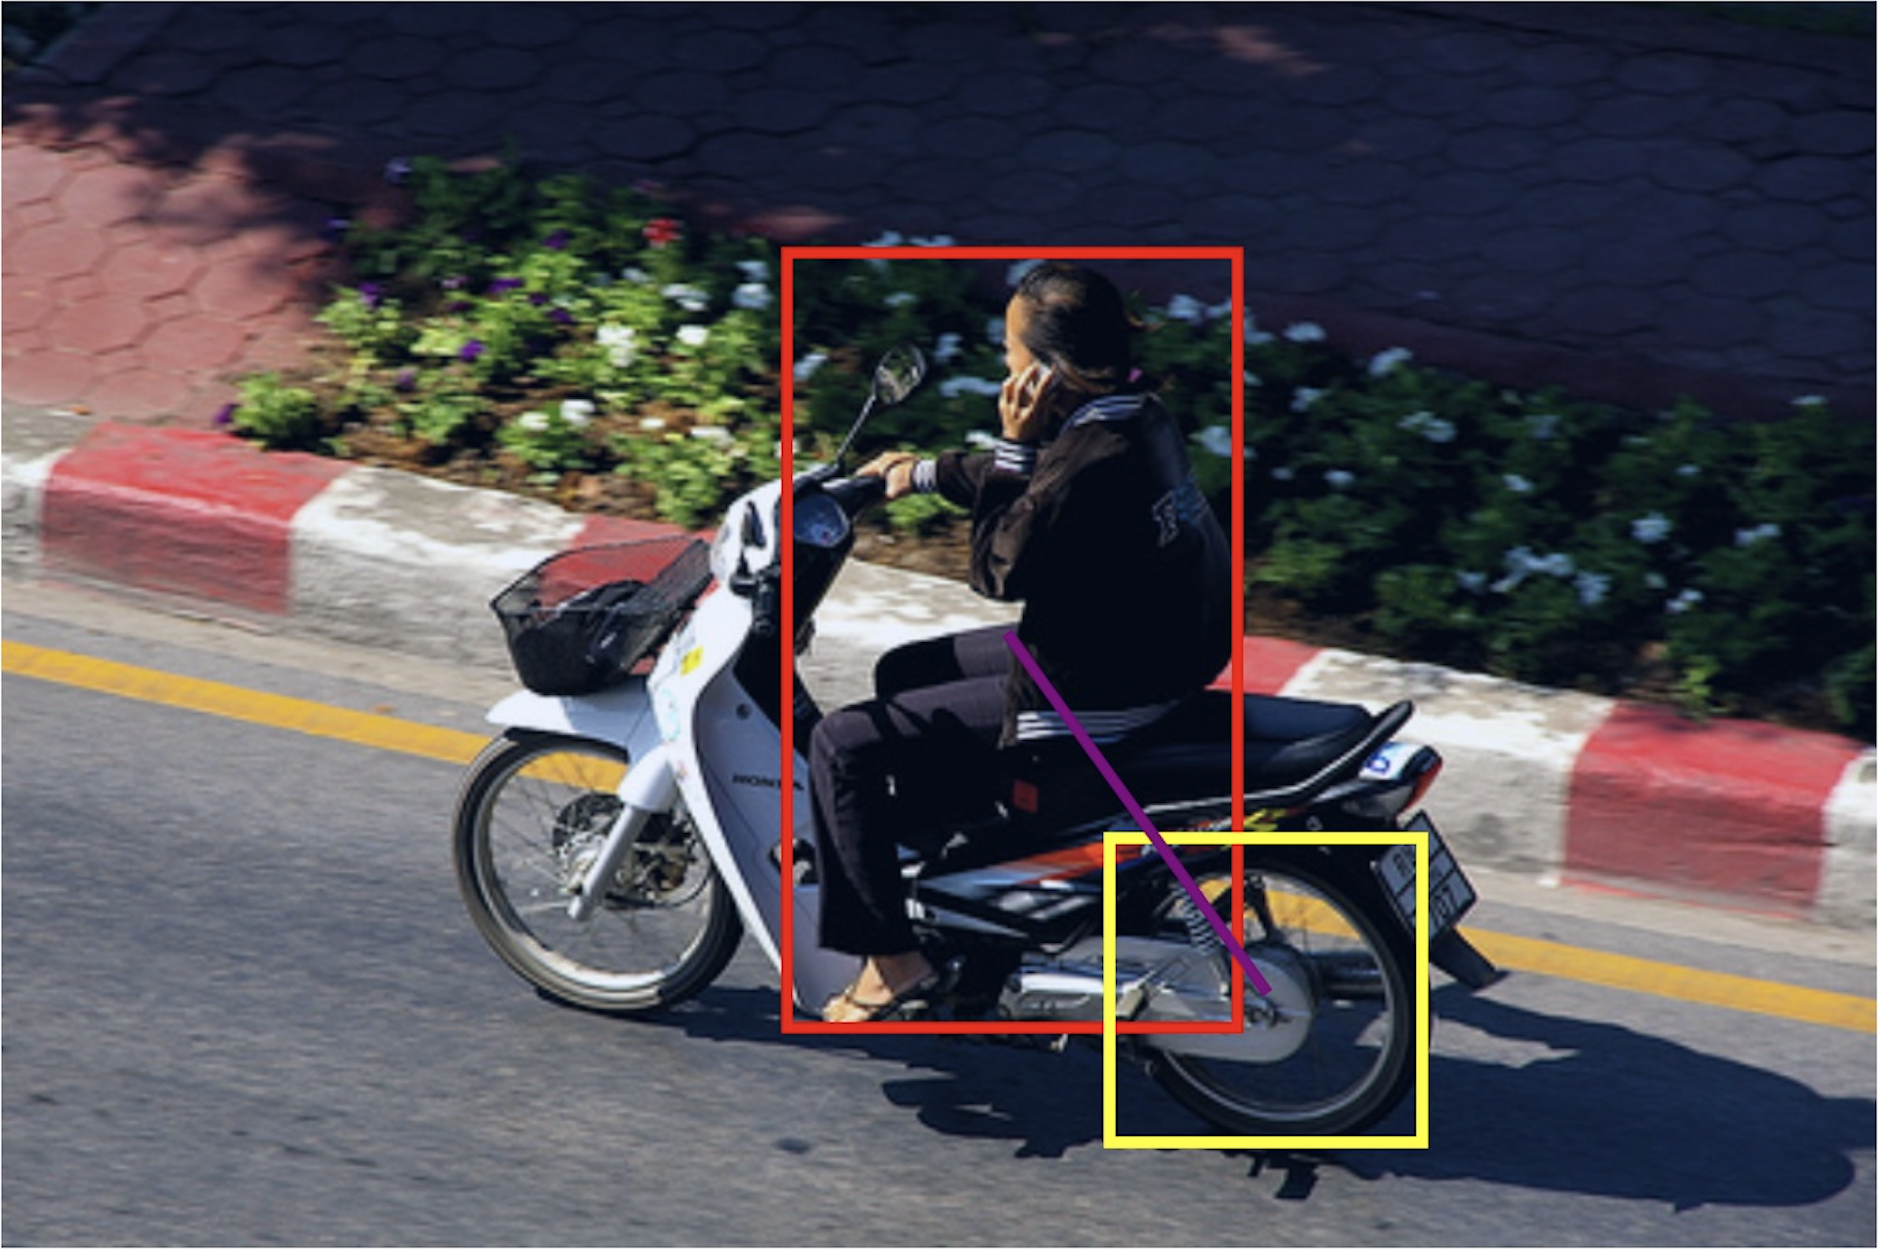
\includegraphics[width=0.9\linewidth]{figures/motor/man1}
			\label{fig:motor_man1}
	\end{minipage}}
	\subfigure[$ <man, \varnothing, wheel_2>  $]{
		\begin{minipage}[t]{5cm}
			\centering
			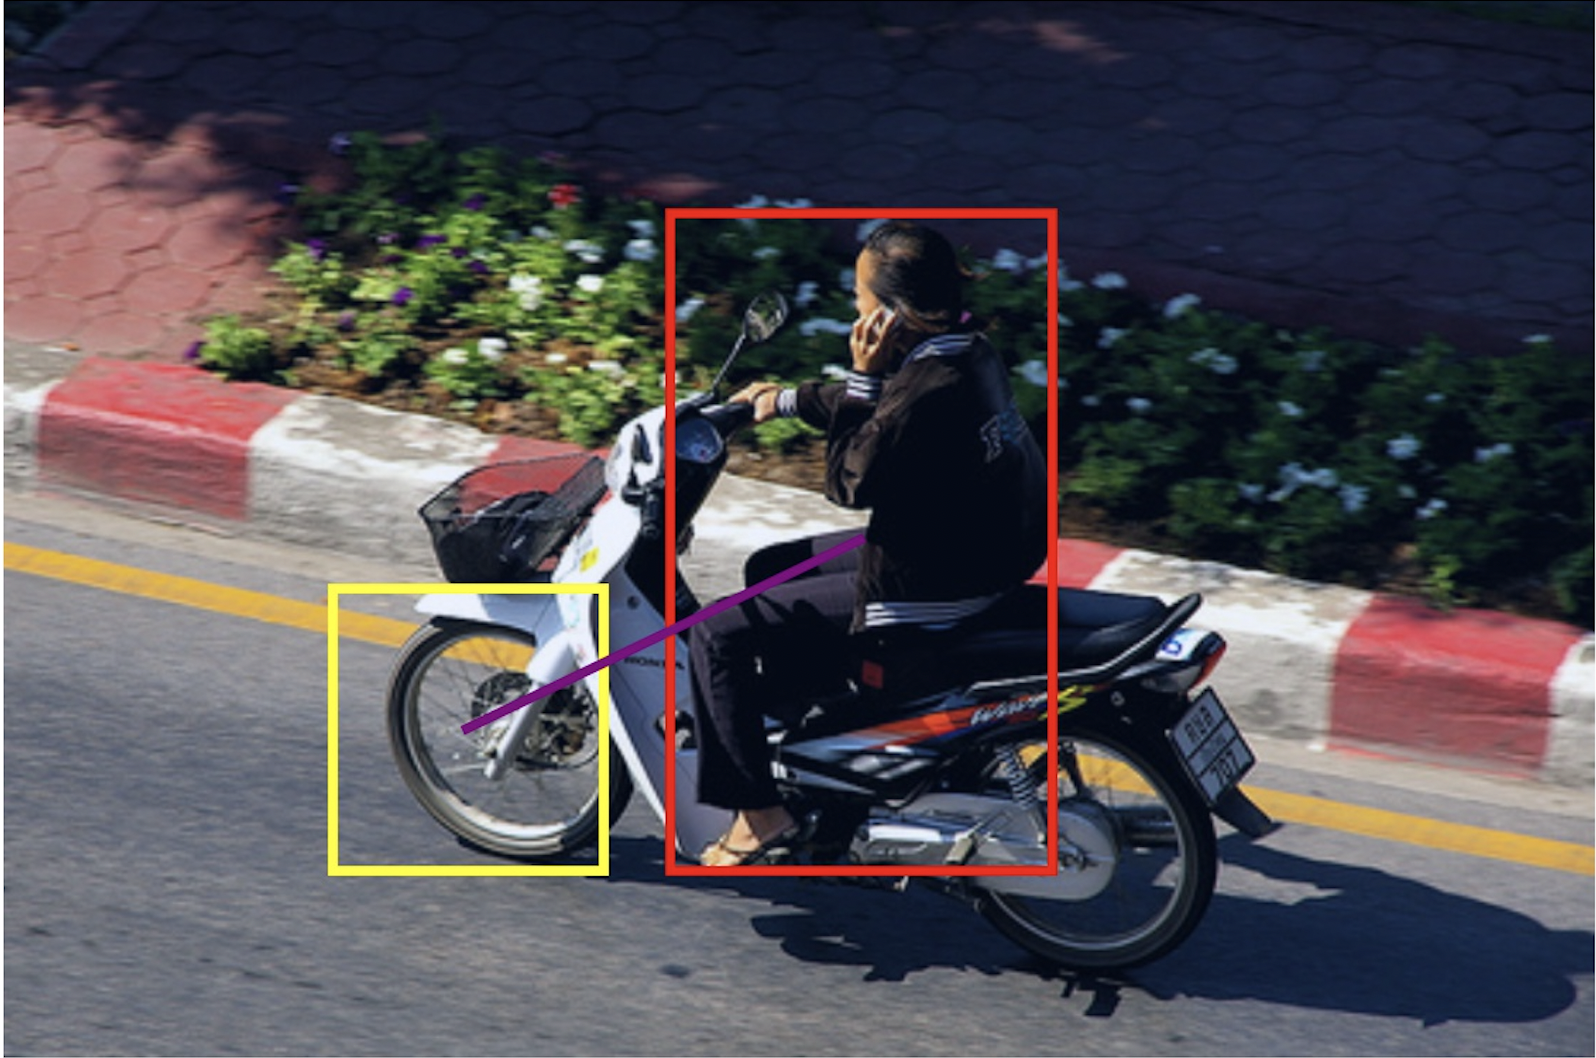
\includegraphics[width=0.9\linewidth]{figures/motor/man2}
			\label{fig:motor_man2}
	\end{minipage}}

	\subfigure[$\forall Attention_{p^i_{man} \to p^j_{bike}} $]{
		\begin{minipage}[t]{5cm}
			\centering
			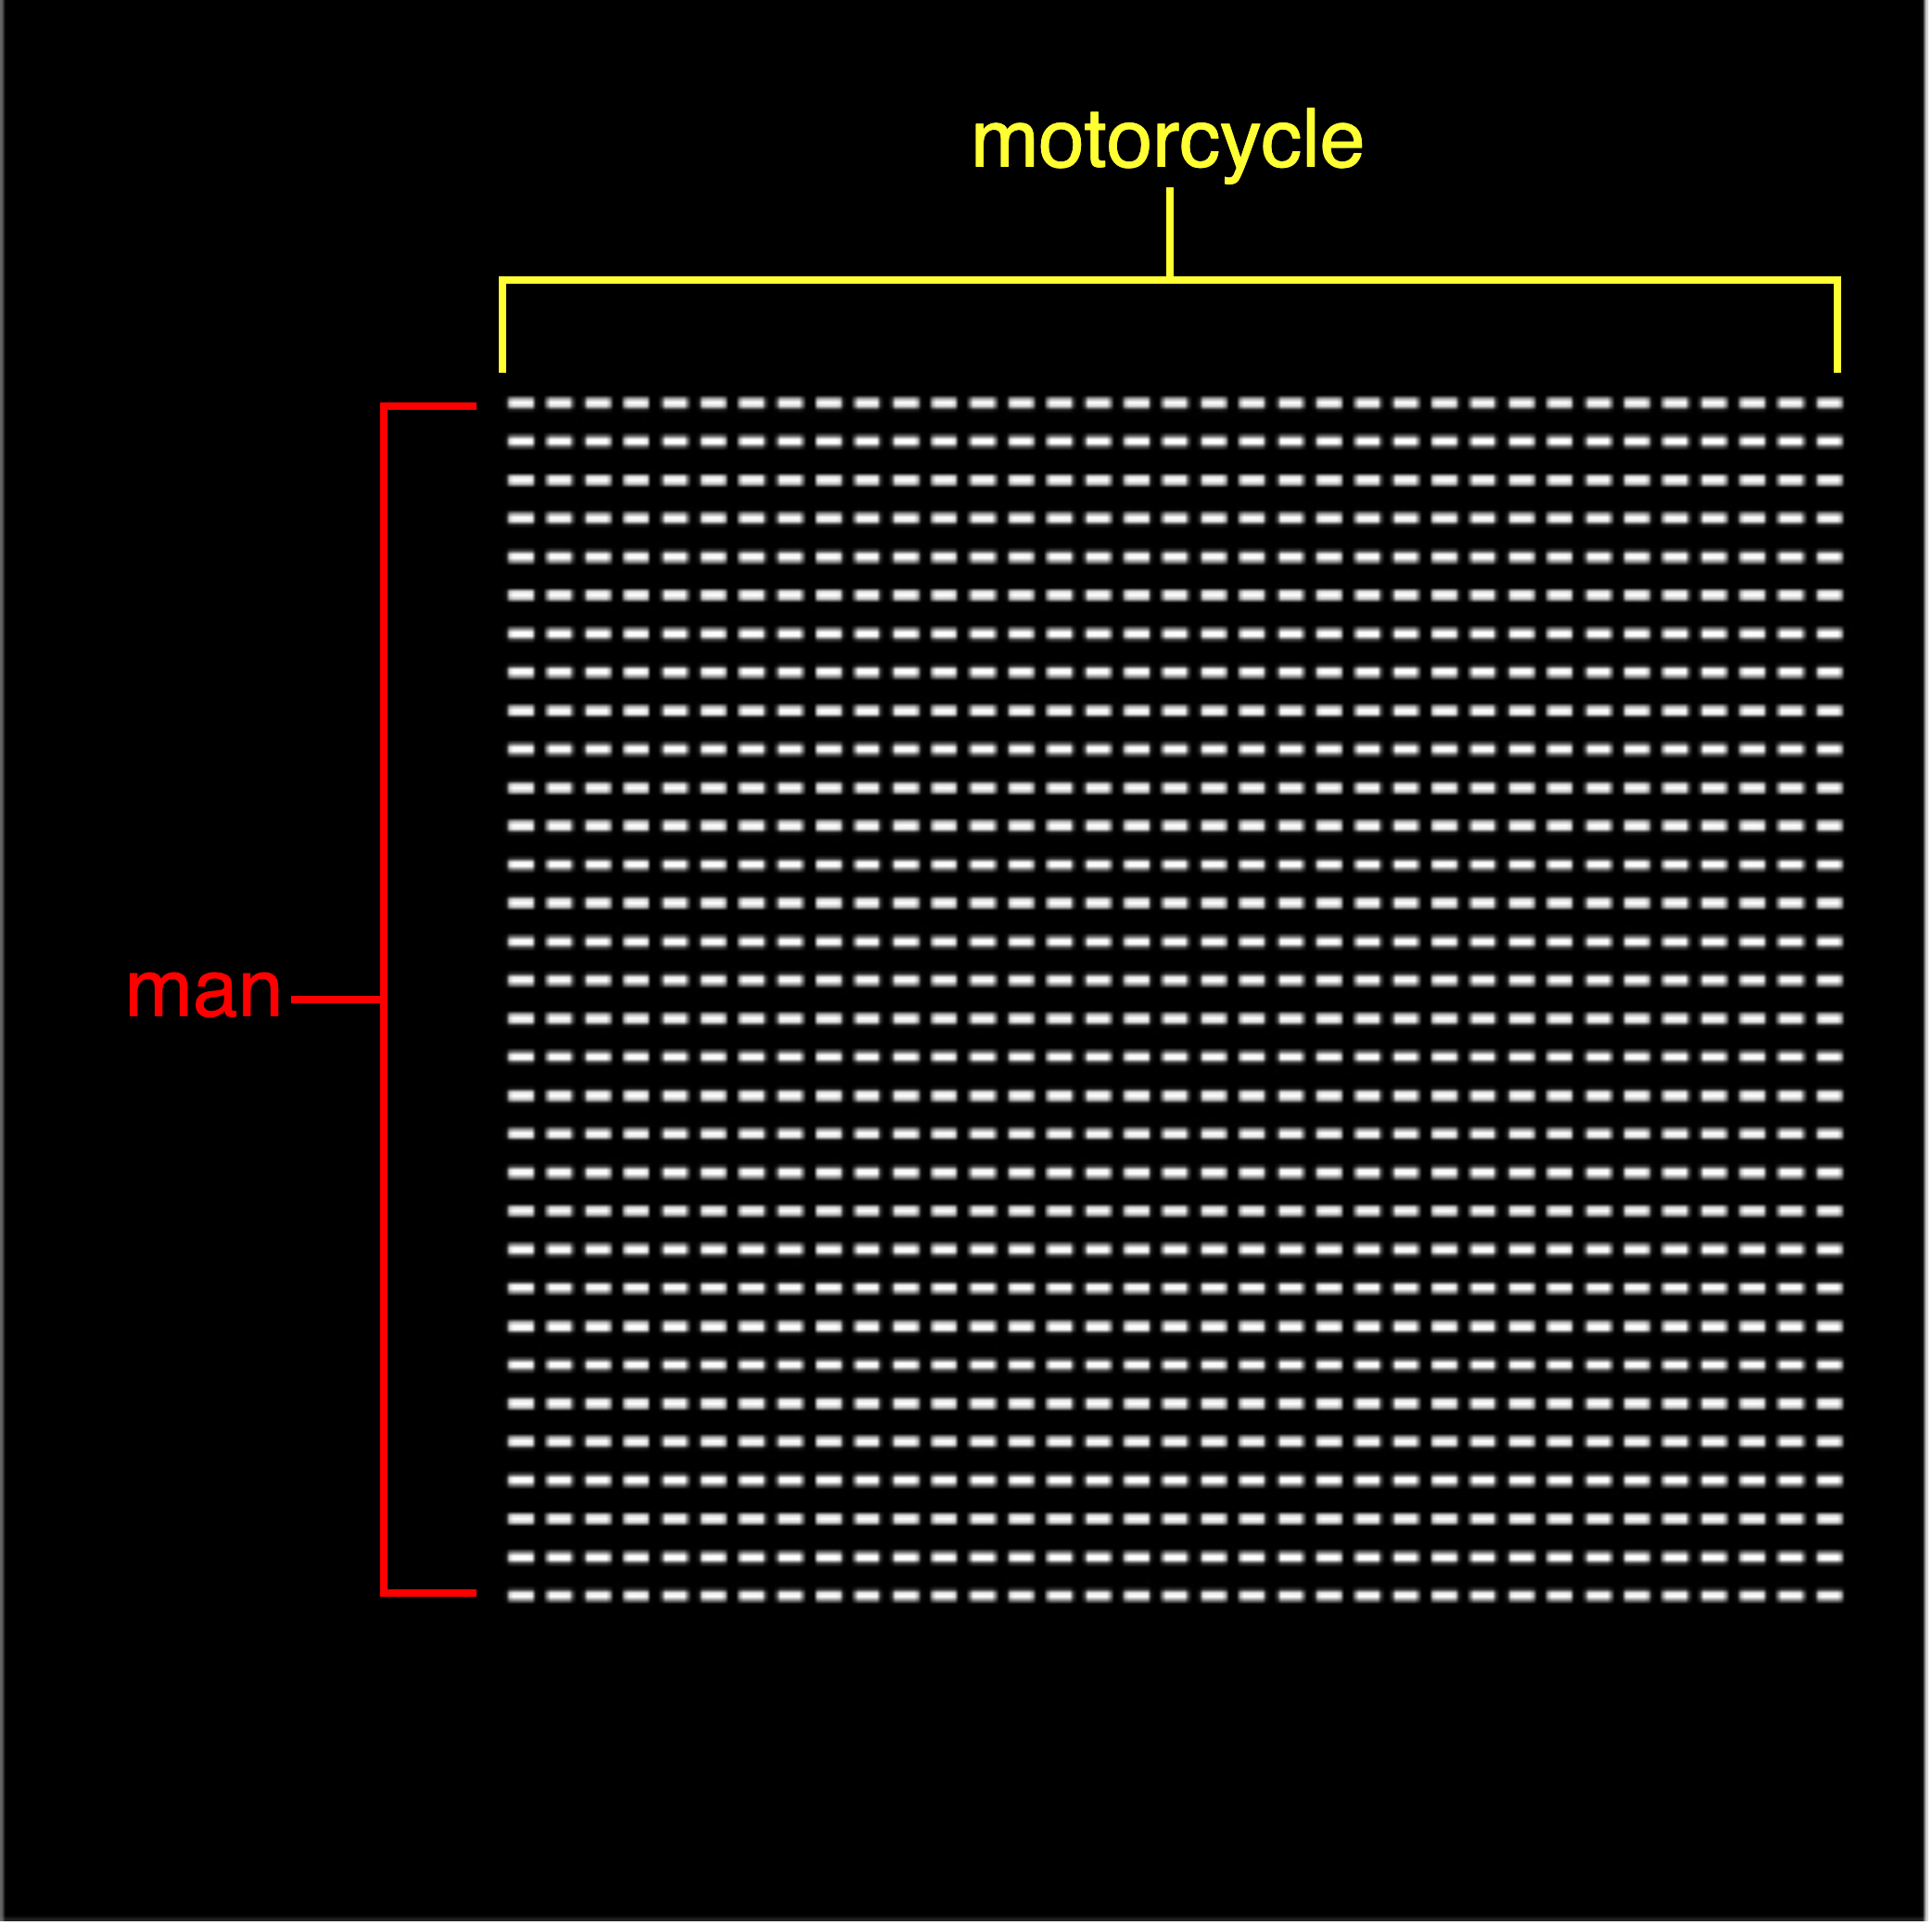
\includegraphics[width=0.9\linewidth]{figures/motor/map0}
			\label{fig:motor_map0}
	\end{minipage}}
	\subfigure[$\forall Attention_{p^i_{man} \to p^j_{wheel_1} } $]{
		\begin{minipage}[t]{5cm}
			\centering
			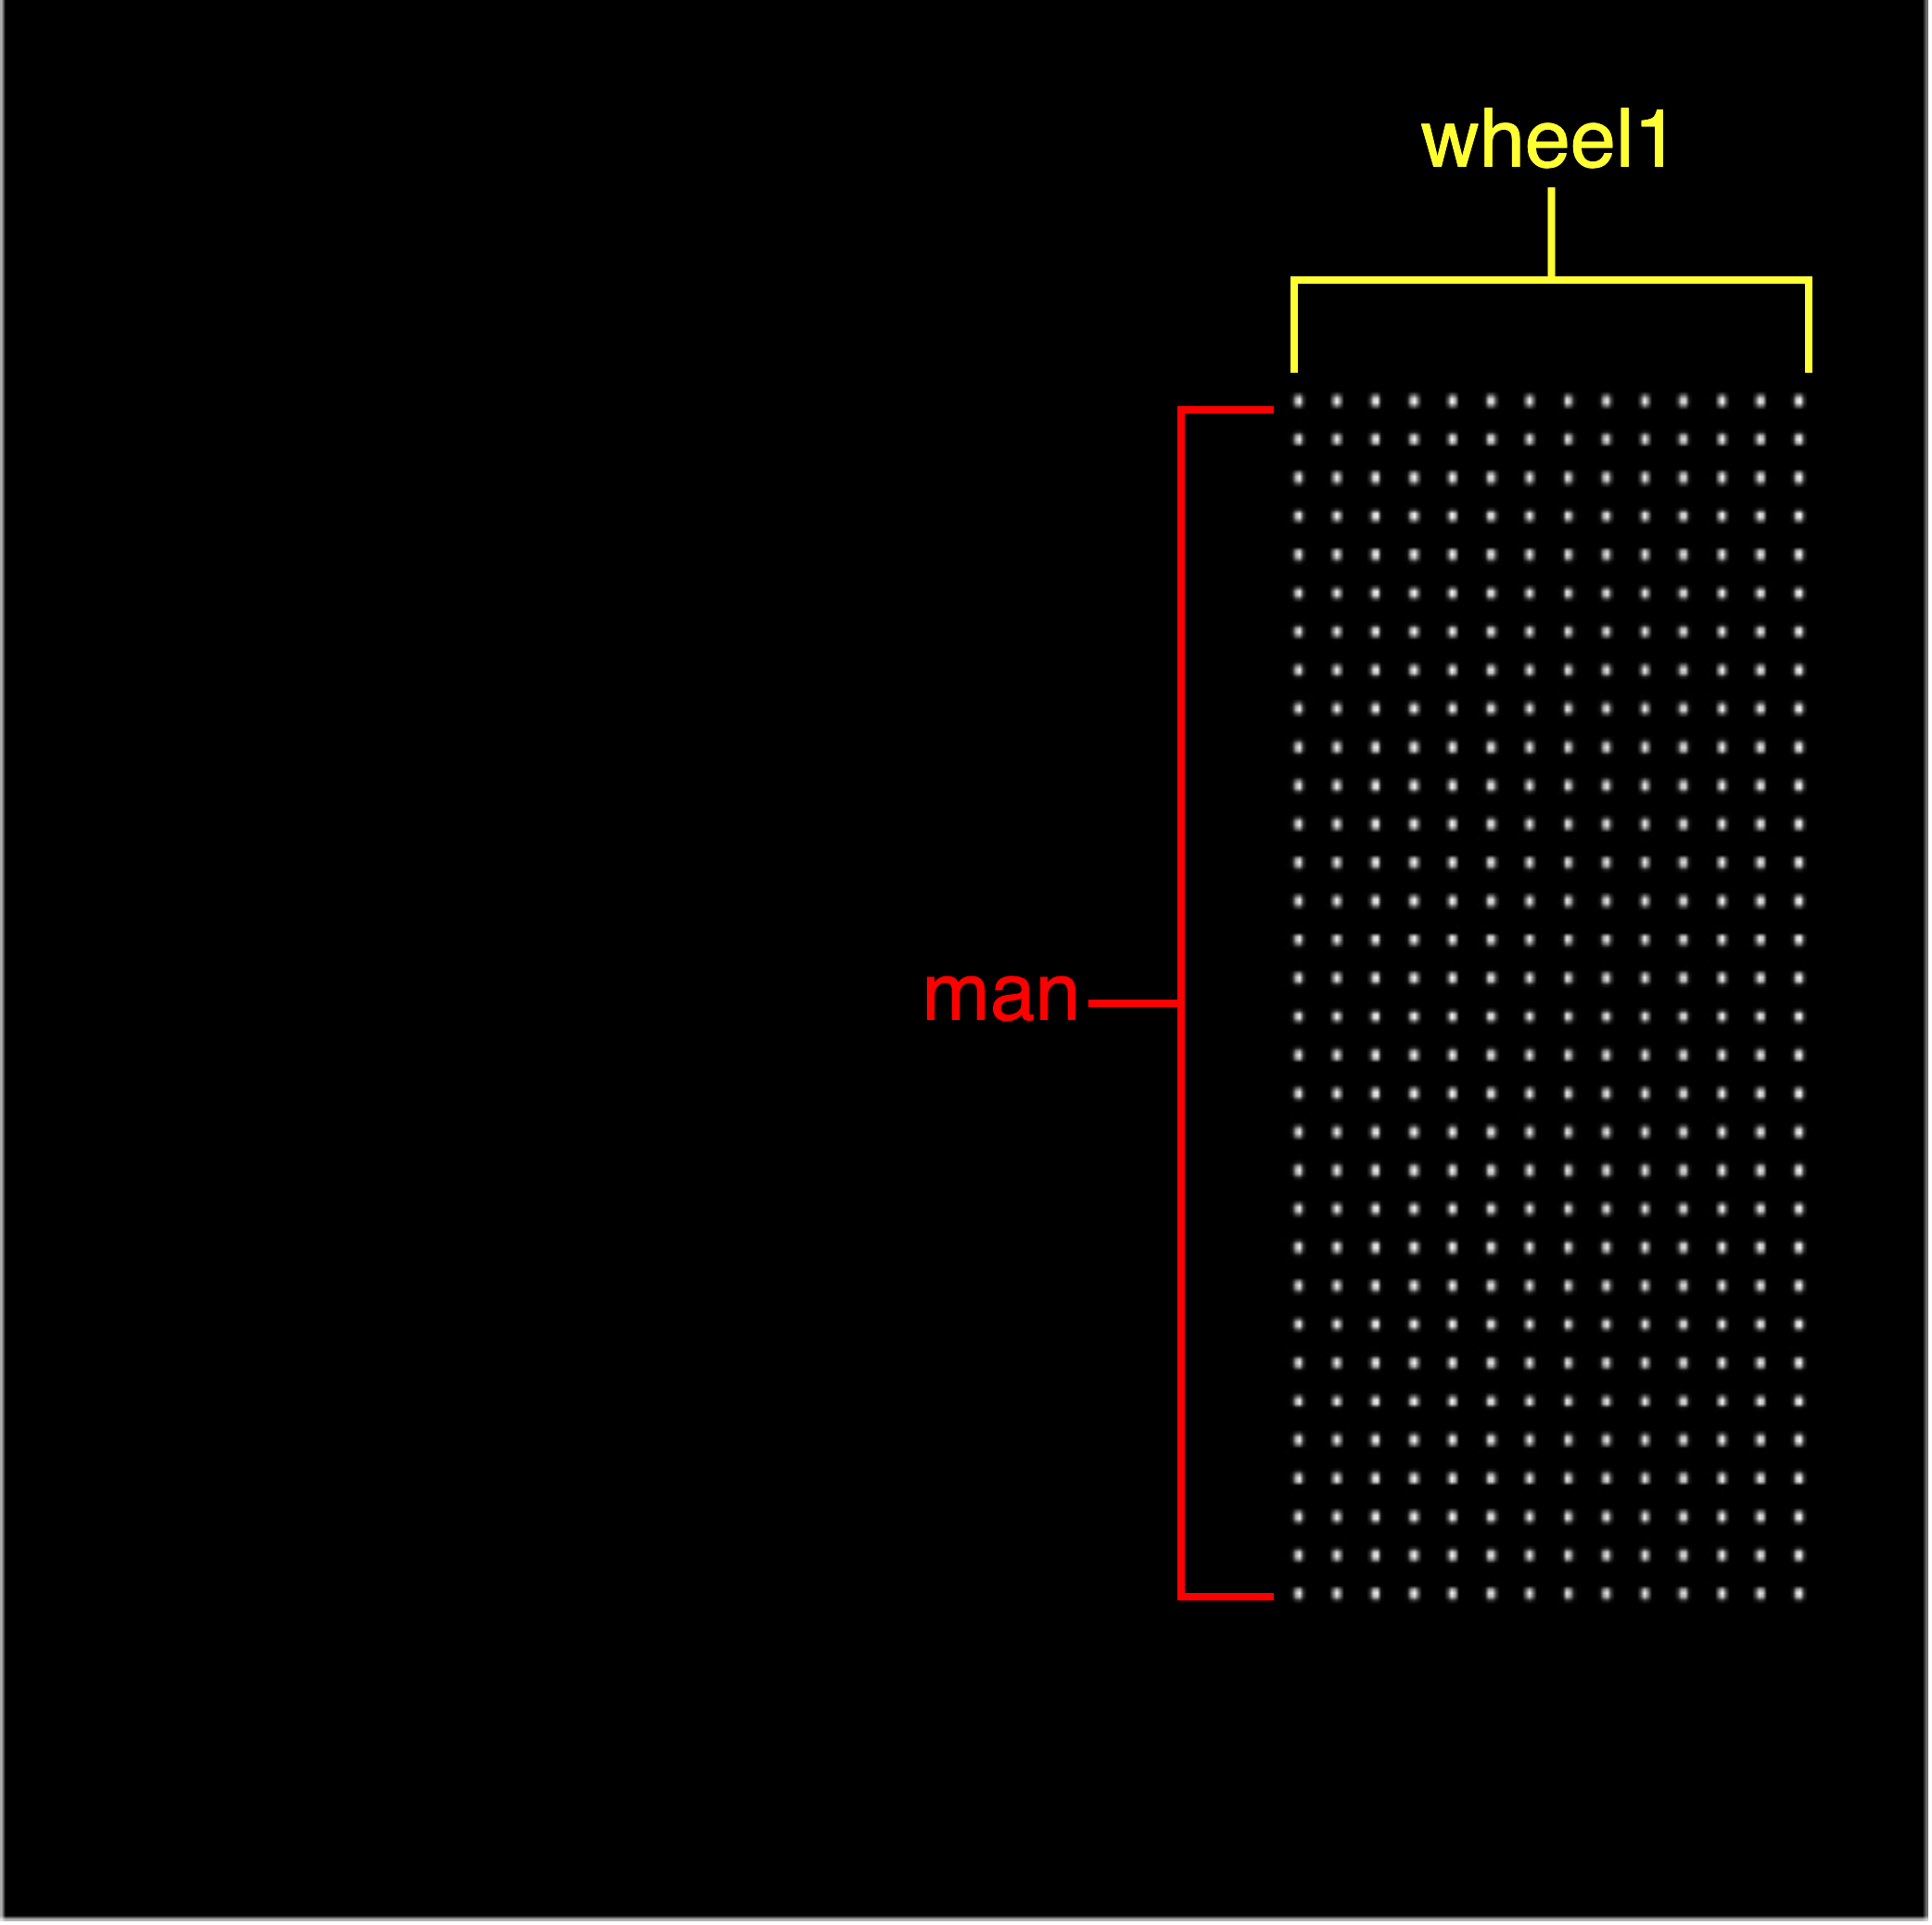
\includegraphics[width=0.9\linewidth]{figures/motor/map1}
			\label{fig:motor_map1}
	\end{minipage}}
	\subfigure[$\forall Attention_{p^i_{man} \to p^j_{wheel_2} } $]{
		\begin{minipage}[t]{5cm}
			\centering
			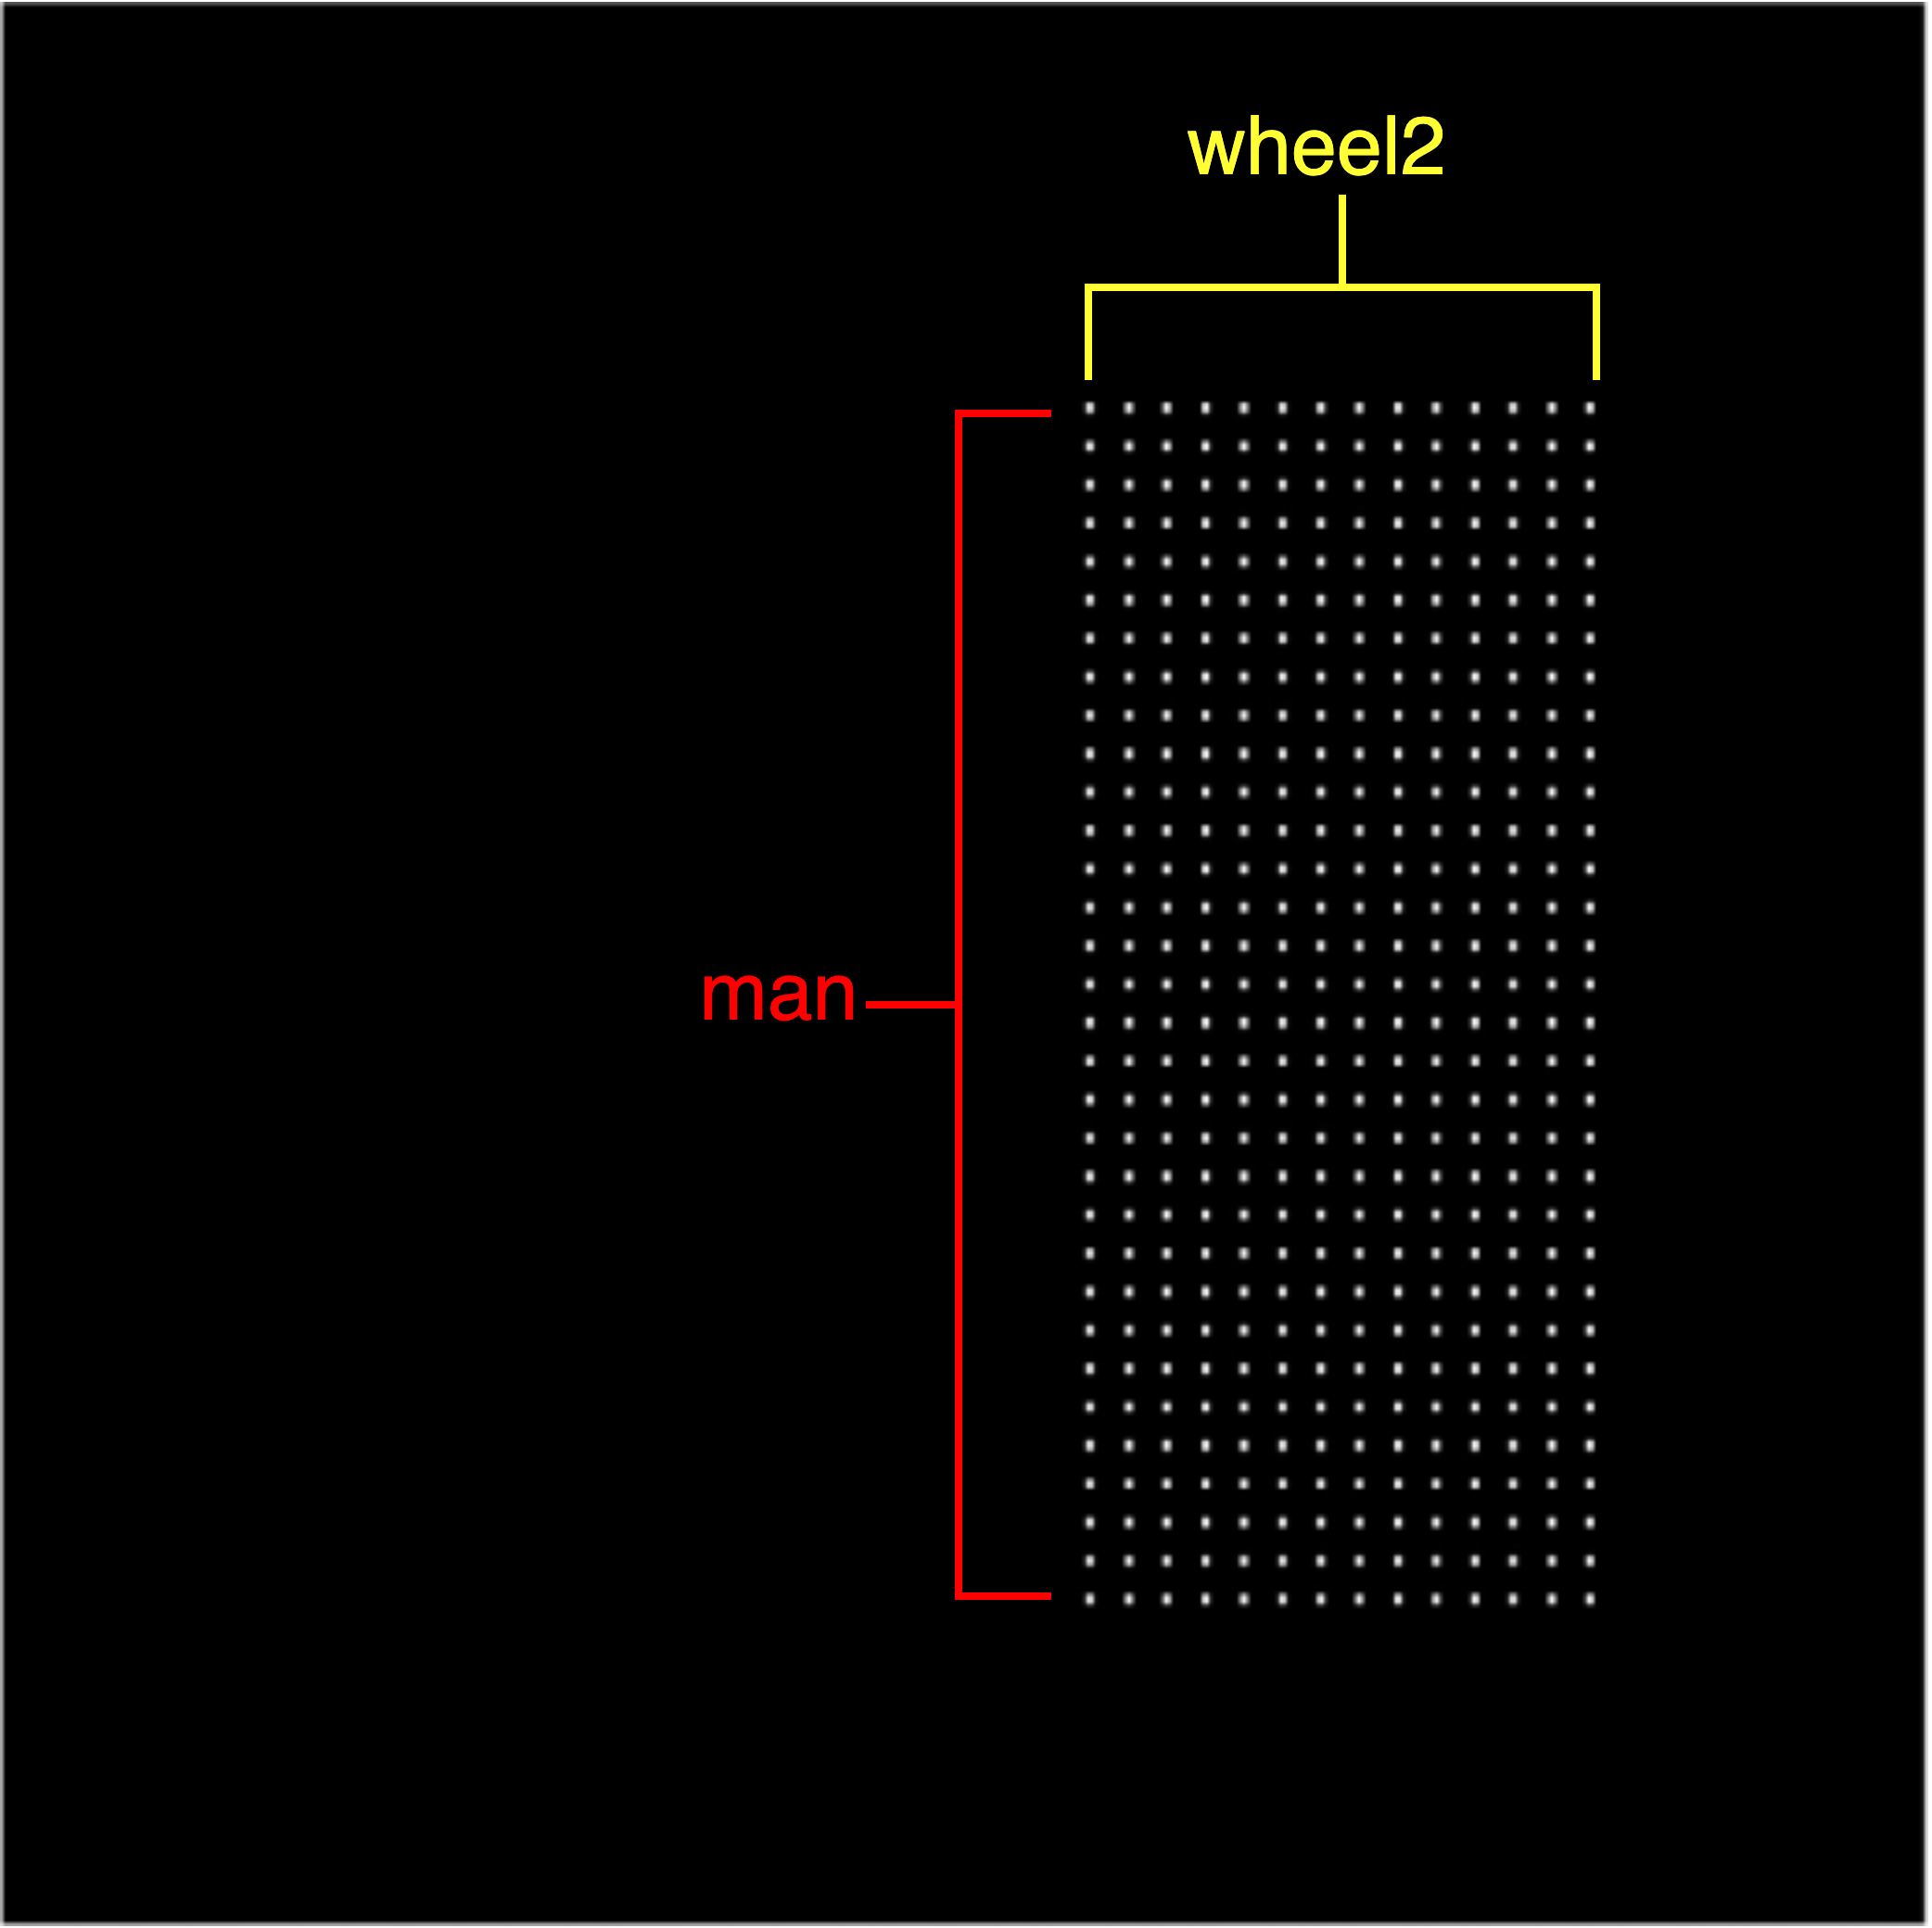
\includegraphics[width=0.9\linewidth]{figures/motor/map2}
			\label{fig:motor_map2}
	\end{minipage}}
	
	\caption[The attention map of each pair.]{The attention map of each pair, where $ (a) $ is the ground truth pair and $ (d) $ is its corresponding position in the attention map. $ (b) $, $(c) $ are no relationship pair, and $ (e) $, $ (f) $ is theirs corresponding positions in the attention map.}
	\label{fig:motor_pair}
\end{figure}

\begin{figure}[tbph!]
	\centering
	\subfigure[ $\forall Att^i_{rel}$]{
		\begin{minipage}[t]{5cm}
			\centering
			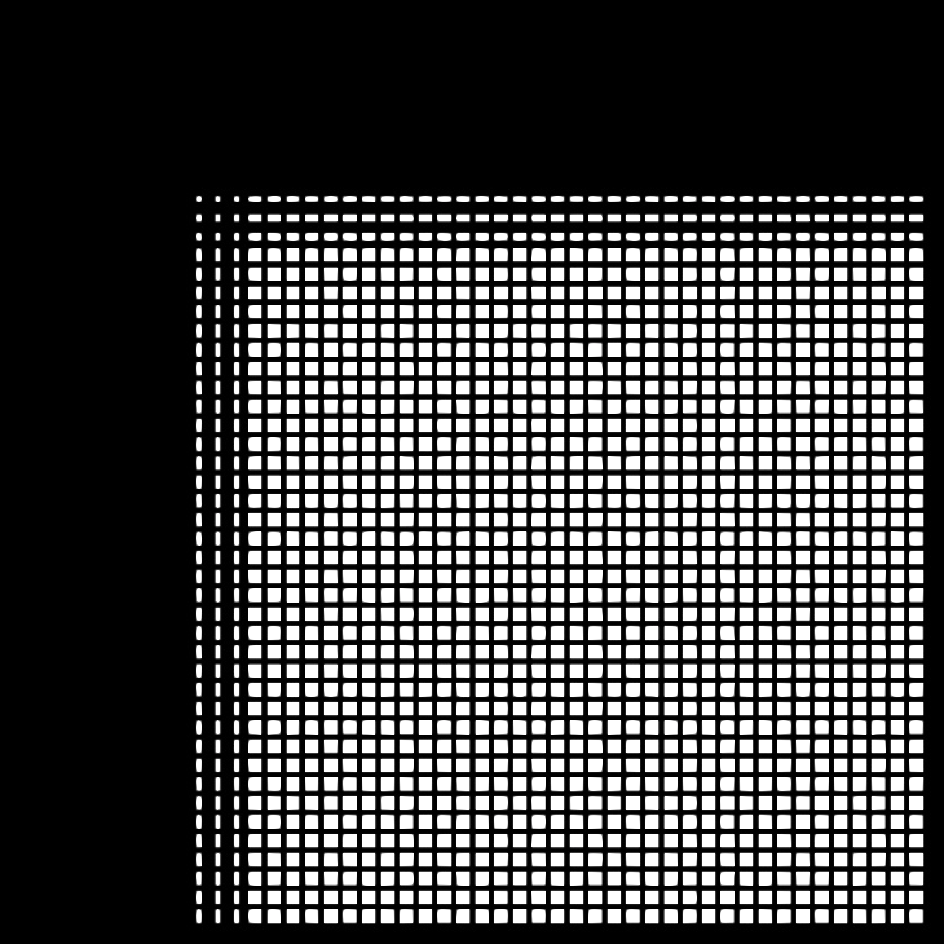
\includegraphics[width=0.9\linewidth]{figures/motor/all0}
			\label{fig:motor_all0}
	\end{minipage}}
	\subfigure[$ \forall Att^i_{no\_rel }$]{
		\begin{minipage}[t]{5cm}
			\centering
			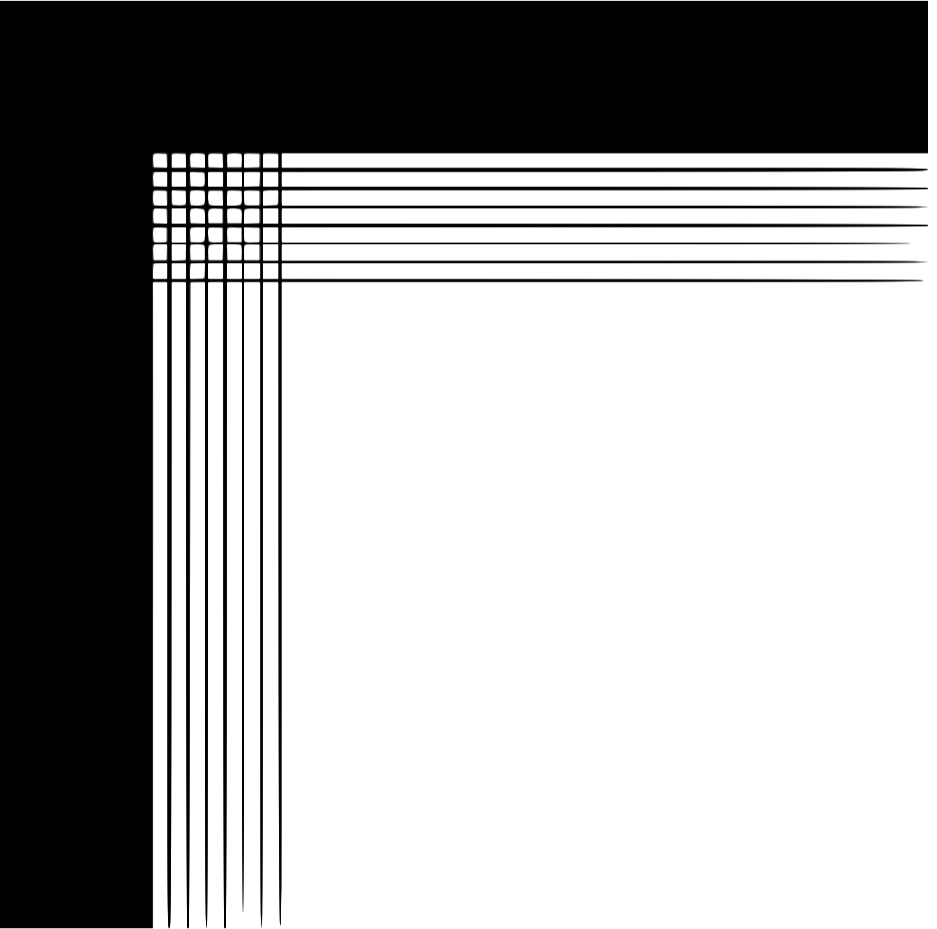
\includegraphics[width=0.9\linewidth]{figures/motor/all1}
			\label{fig:motor_all1}
	\end{minipage}}
	\subfigure[$ \forall Att^i_{rel} \cap  \forall Att^i_{no\_rel } $]{
		\begin{minipage}[t]{5cm}
			\centering
			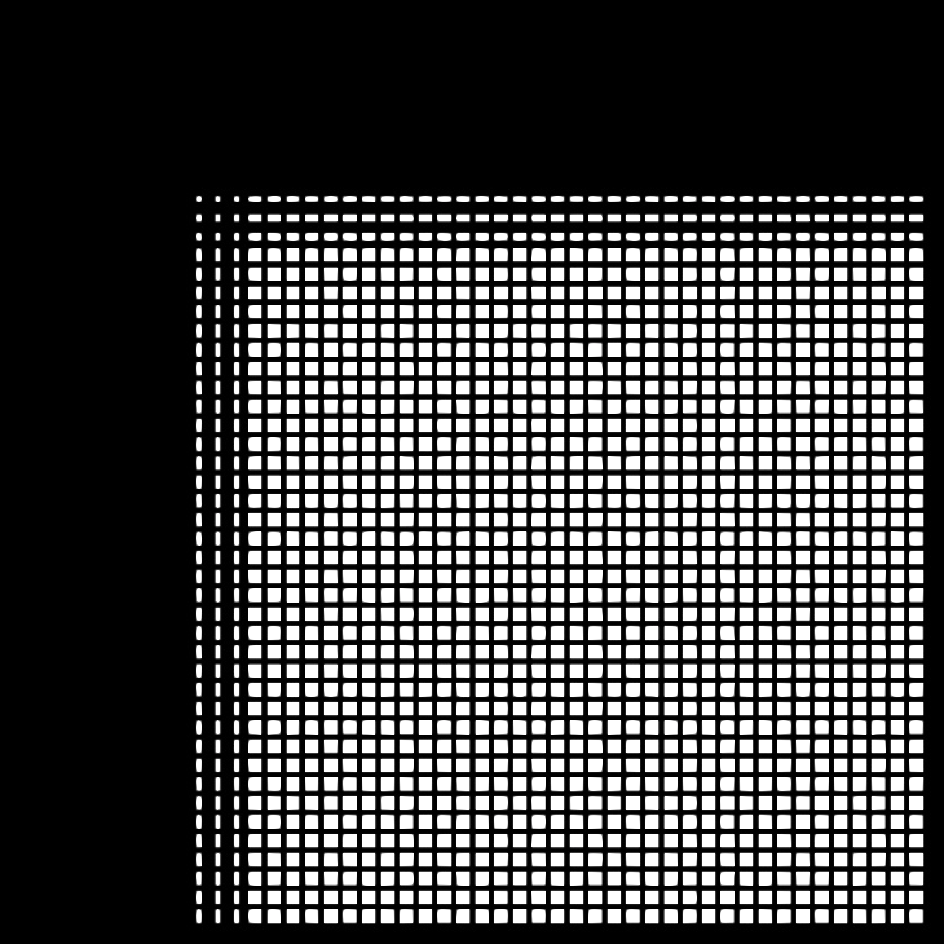
\includegraphics[width=0.9\linewidth]{figures/motor/all0}
			\label{fig:motor_all2}
	\end{minipage}}
	
	\caption[The overlap in Attention map]{The overlap in Attention map.The sub-figure (a) is the attention of all the related pairs, and the sub-figure (b) is the attention of all the irrelevant pairs. The sub-figure(c) shows that there is a serious overlap between them. We cannot increase the attention shown in (a) and decrease the attention of (b) through our attention loss.}
	\label{fig:overlap}
\end{figure}



\section{Experiments on Proposed Framework}

As mentioned above, our Pixel-based Attention idea was not able to meet our expectations due to the overlap, so we modified the model and designed Retina net.  
In this section, we introduce in detail the relevant experiments and results of Retina Net, including experiments on box query, attention map, relation decoder, as well as the parameter adjustment of the transformer, and the final result comparison.

\subsection{Implementation details}
 The model is implemented in $ pythorch\-0.4 $~\cite{paszke2019pytorch}. The input of the model is the same as Motifs-Net~\cite{zellers2018neural} , that is an image with a size of $ 592 \times 592 $. VGG16~\cite{simonyan2015deep} backbone pretrains the Visual Genome~\cite{krishna2017visual} dataset. As mentioned in  Sec.~\ref{sec:retinanet}, the encoder and the two decoder modules accept input features of size 2048. There are 3x Encoder, 3x Object Decoder , 3x Relation Decoder and 8 attention heads for transformer network. The GloVe vector embedding has size 200. SGD with momentum along with learning rate of $ 10^{-3 }$ and the batch size is 6. And cross-entropy loss function is adopted to compute the object and relation classification loss.

 We have followed three standard evaluation modes same as in current benchmark of the Motifs-Net~\cite{zellers2018neural} : (1) \textbf{predicate classification} (PredCLS): given a ground truth set of boxes and labels, predict relationship labels, (2) \textbf{scene graph classification} (SGCLS): given ground truth boxes, predict box labels and relationship label and (3) \textbf{scene graph detection} (SGDET): predict boxes, box labels, and relationship labels.
%For the  SGDET, we use a learnable object query, and use the Hungarian matching algorithm to match each object feature. For the other two subtasks\textbf{(setting)}, we use our custom object query to obtain the object feature.


\subsection{Experiment on Object Decoder}

The feasibility of our proposed object query to replace learnable query should be analyzed. The  PredCLS has classes and bounding boxes information, so we designed several object queries based on the known information, as shown in Fig.~\ref{fig:objectquery}, Fig.~\ref{fig:objquery1} and Fig.~\ref{fig:objquery2}. They are called  \textit{objec query 1} ,  \textit{objec query 2} , and  \textit{objec query 3}  respectively. Their pros and cons, and their substitutability are discussed  as follows.

The object query 1 mentioned in Sec.~\ref{sec:objectdecoder} has the spatial information of the entity, while the object query 2 is to add a class word embedding on its basis, so that our object query has semantic information. And object query 3 is obtained by a simple linear layer from the bounding box. Each entity in the picture has its own object query, because the object query depends on the bounding box.

\begin{figure}[tbph!]
	\centering
	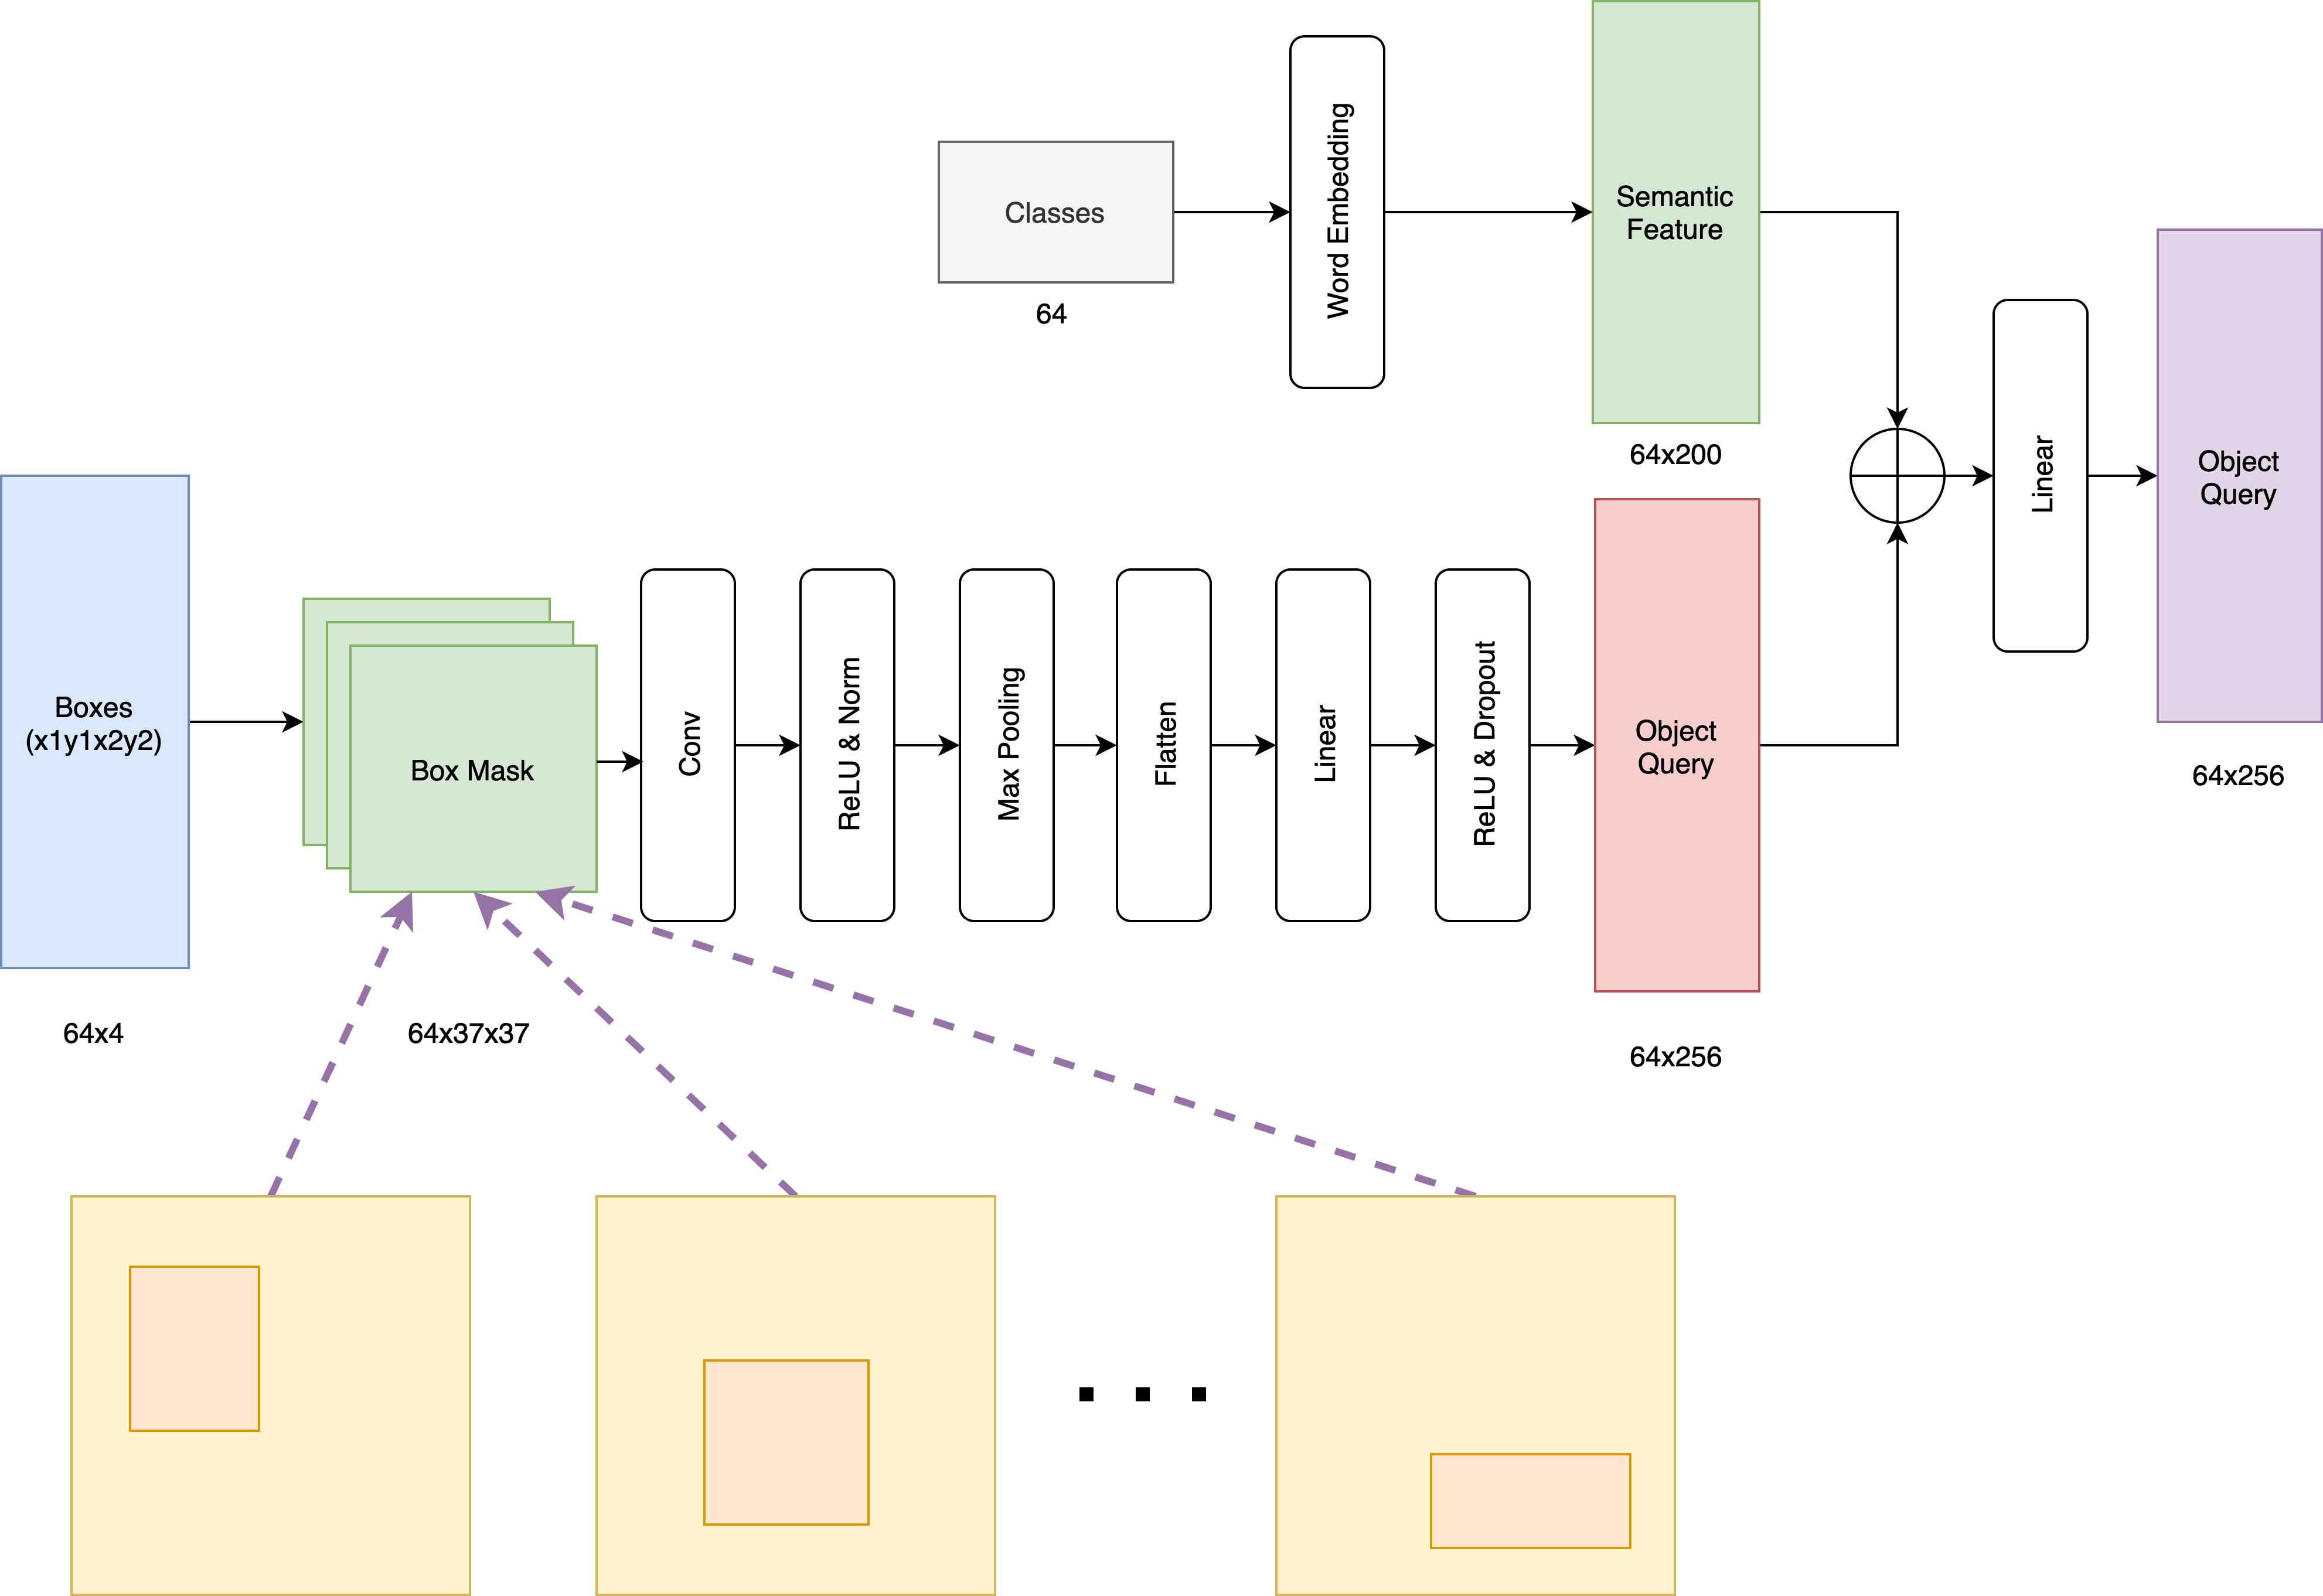
\includegraphics[width=0.8\linewidth]{figures/obj_query1}
	\caption[Illutrastion of the object query 2]{Illutrastion of the object query 2. Compared with object query1 in Fig.~\ref{fig:objquery1}, it integrate the semantic feature of objects.}
	\label{fig:objquery1}
\end{figure}

\begin{figure}[tbph!]
	\centering
	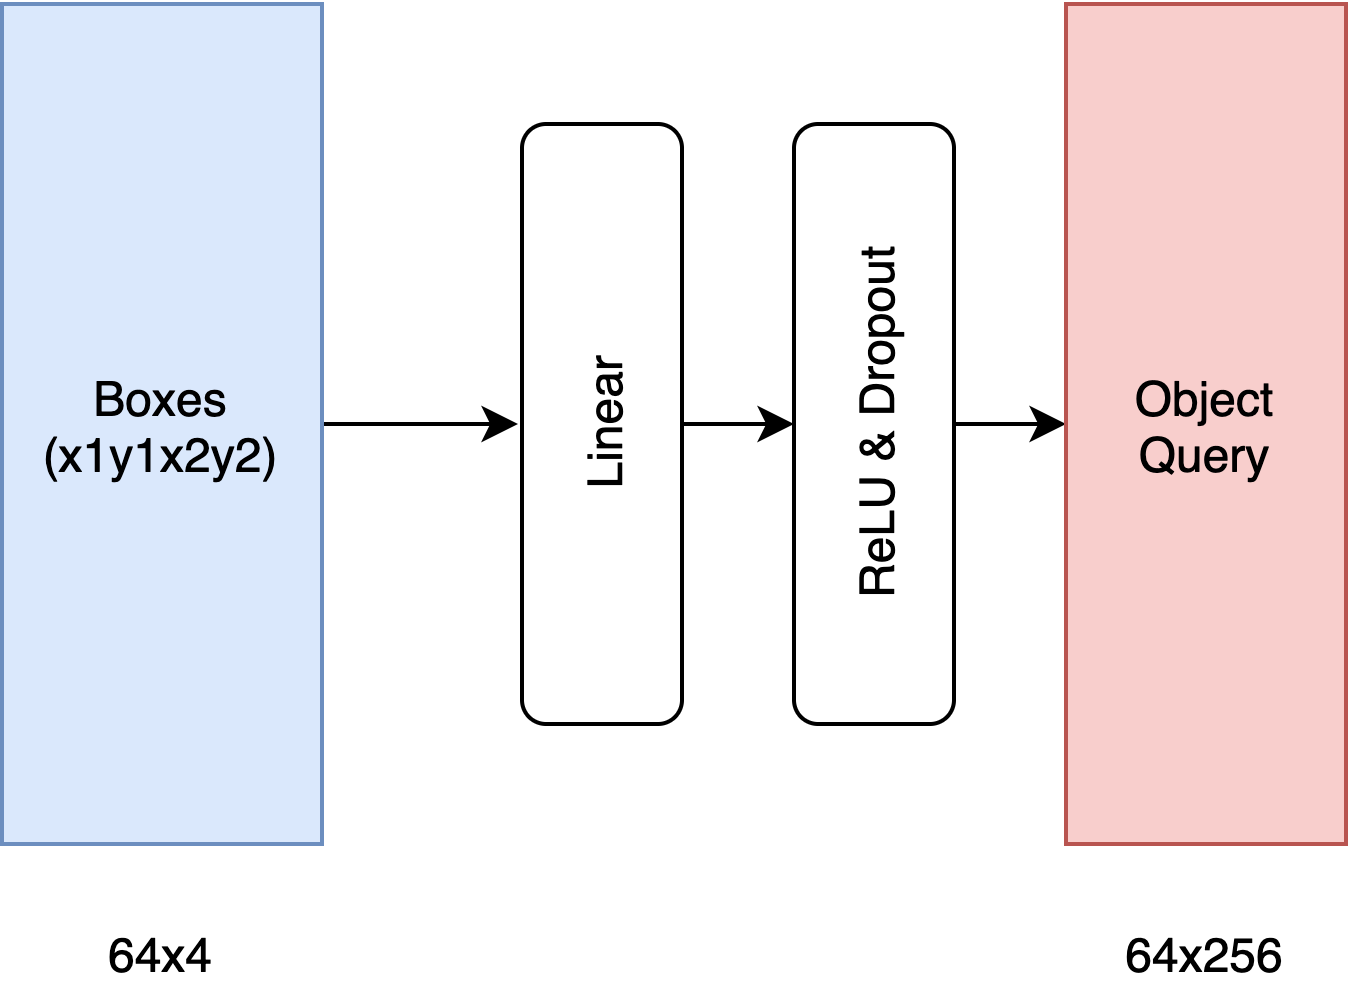
\includegraphics[width=0.5\linewidth]{figures/obj_query2}
	\caption[Illutrastion of the object query 3]{Illutrastion of the object query 3,we only added a simple linear layer behind the bounding box.}
	\label{fig:objquery2}
\end{figure}

\subsubsection{Consistency of the Object Query }

DETR uses a learnable embedding vector as the query,and it utilizes the Hungarian matching algorithm to find the most matching object feature, because their queries have no actual physical meaning, and the queries are fixed for each picture and cannot establish a direct connection with the actual object.%且对于每一张图片他都是固定的,无法与实际的object 建立直接的联系。
However,since our object query contains relevant information of each object, such as spatial information and semantic information, it is in one-to-one correspondence with the entities in the picture.

In order to verify the correspondence between the object query and the entity in the picture, a box regression is designed in the experiment. After the object query and object feaure, two Multilayer Perceptron(MLP) modules are separately added, and then observe whether they can regain the spatial information of the object.For the evaluation metrics, IoU and GIoU~\cite{rezatofighi2019generalized} are used .

After the MLP, a bounding box vector $ \hat{b_\sigma} $ is obtained, then the box loss $\mathcal{L}_{box}$can be calculated with ground truth bounding box $b$. The box loss consists of a GIoU loss $  \mathcal{L}_{GIoU} $ and a $l_1$ loss, see the following equation:

$$ \mathcal{L}_{box}(b,\hat{b}_{\hat{\sigma}}) = \mathcal{L}_{GIoU}(b,\hat{b}_{\sigma}) + \left \| b - \hat{b}_{\sigma}  \right \| _1 $$

\begin{table}[!h]
	\centering
	\begin{tabular}{c|ccc}
		\bottomrule
		& object query 1 & object query 2 & object query 3  \\ \midrule
		IoU  & 0.759  & 0.750  & 0.681    \\
		GIoU & 0.744  & 0.733 & 0.669   \\ \midrule
		&object feature 1  &object feaure 2 & object feautre 3\\ \midrule
		IoU & 0.634 & 0.631 & 0.580 \\
		GIoU	& 0.617 & 0.620 & 0.568  \\\bottomrule
		
	\end{tabular}
\caption[The regression result of the object query and feature]{The regression result of the object queries and features.}
\label{tab:regresstion}
\end{table}

Table~\ref{tab:regresstion} shows that the IoU of object queries can reach 0.75 and the IoU of object features averages 0.6. This verifies that there is a one-to-one correspondence between all three object queries and objects, and the object query 3 is slightly worse than the others.

\subsubsection{The comparison of object queries}
The object query is a $ 64 \times 256 $ matrix, corresponding to the objects in each image, so  each object query can be reshaped into a size of $16 \times 16$ image. Fig.~\ref{fig:tennis}  shows that three different queries are generated through three different methods, and the query corresponding to each object is also different. For example, in Figure(b), as the area of our entities gradually increases, the query gradually becomes denser. 


\begin{figure}[h!]
	\centering
	\subfigure[The objects with bounding boxes.]{
		\begin{minipage}[t]{3.5cm}
			\centering
			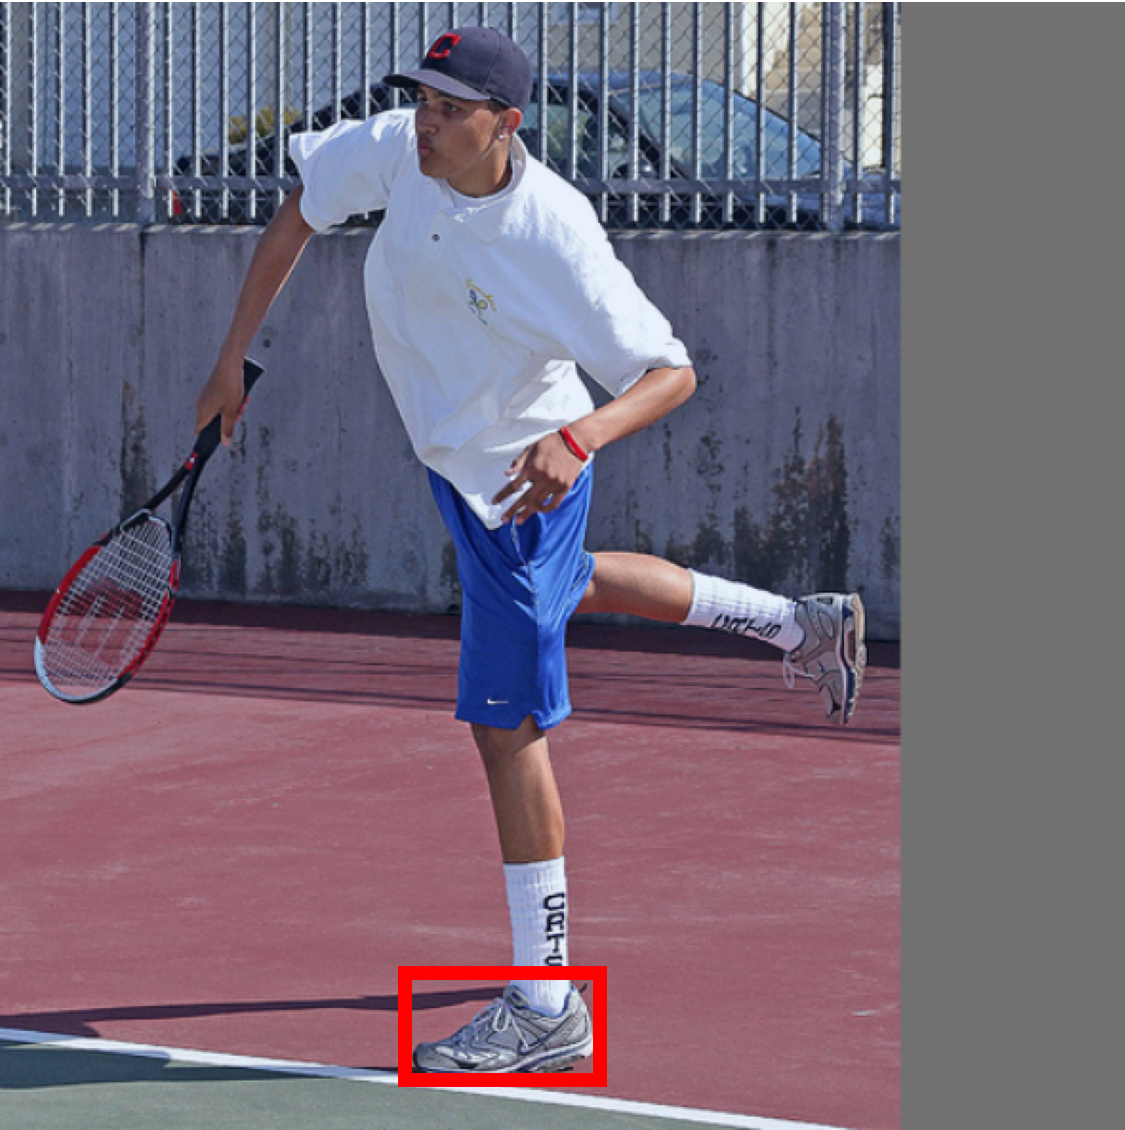
\includegraphics[width=0.9\linewidth]{figures/result/tennis/obj2}
	\end{minipage}
		\begin{minipage}[t]{3.5cm}
			\centering
			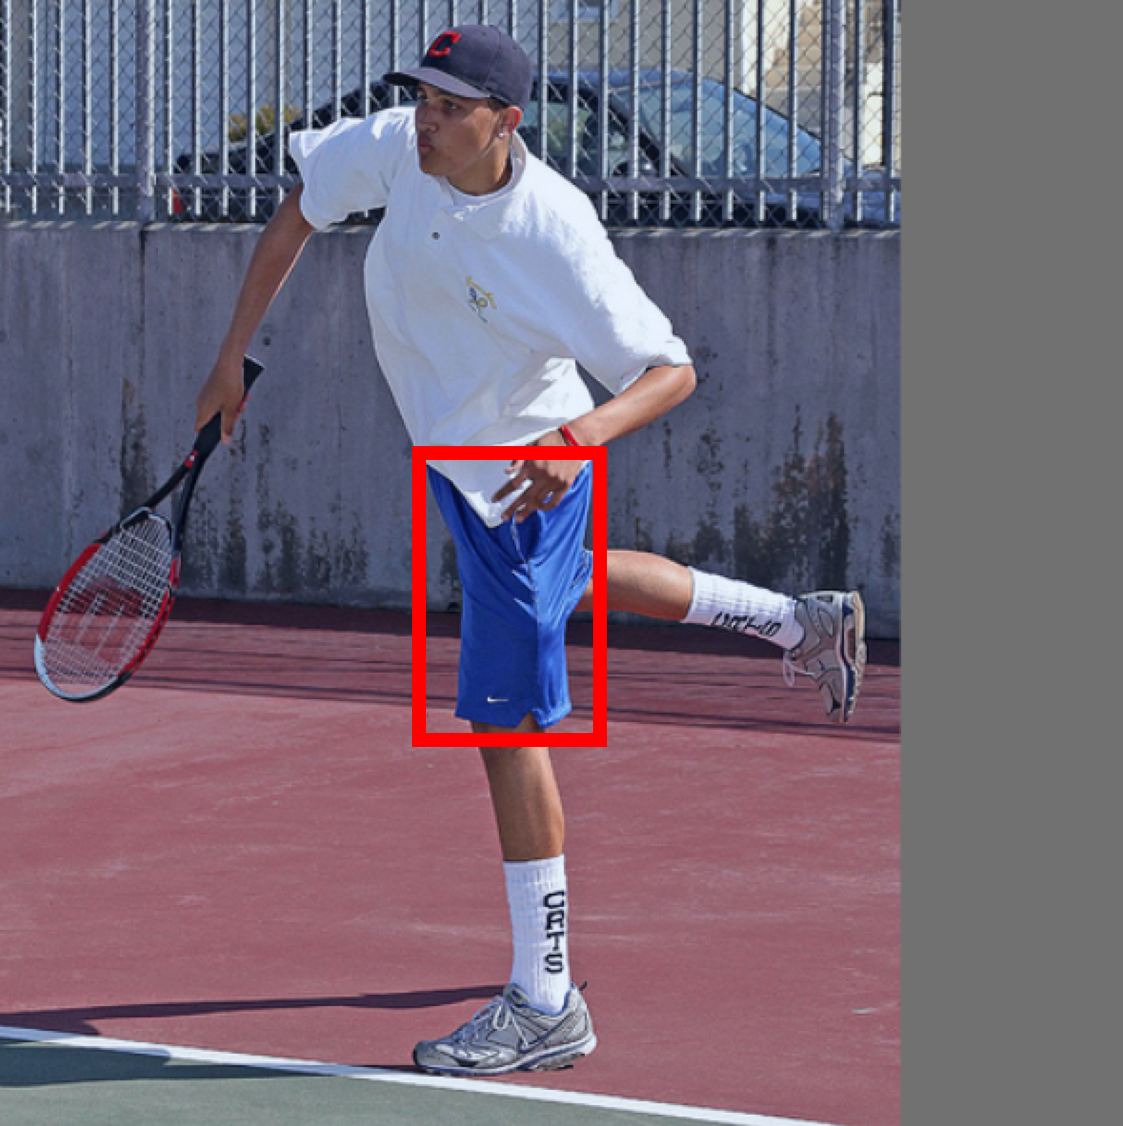
\includegraphics[width=0.9\linewidth]{figures/result/tennis/obj4}
	\end{minipage}
	\begin{minipage}[t]{3.5cm}
		\centering
		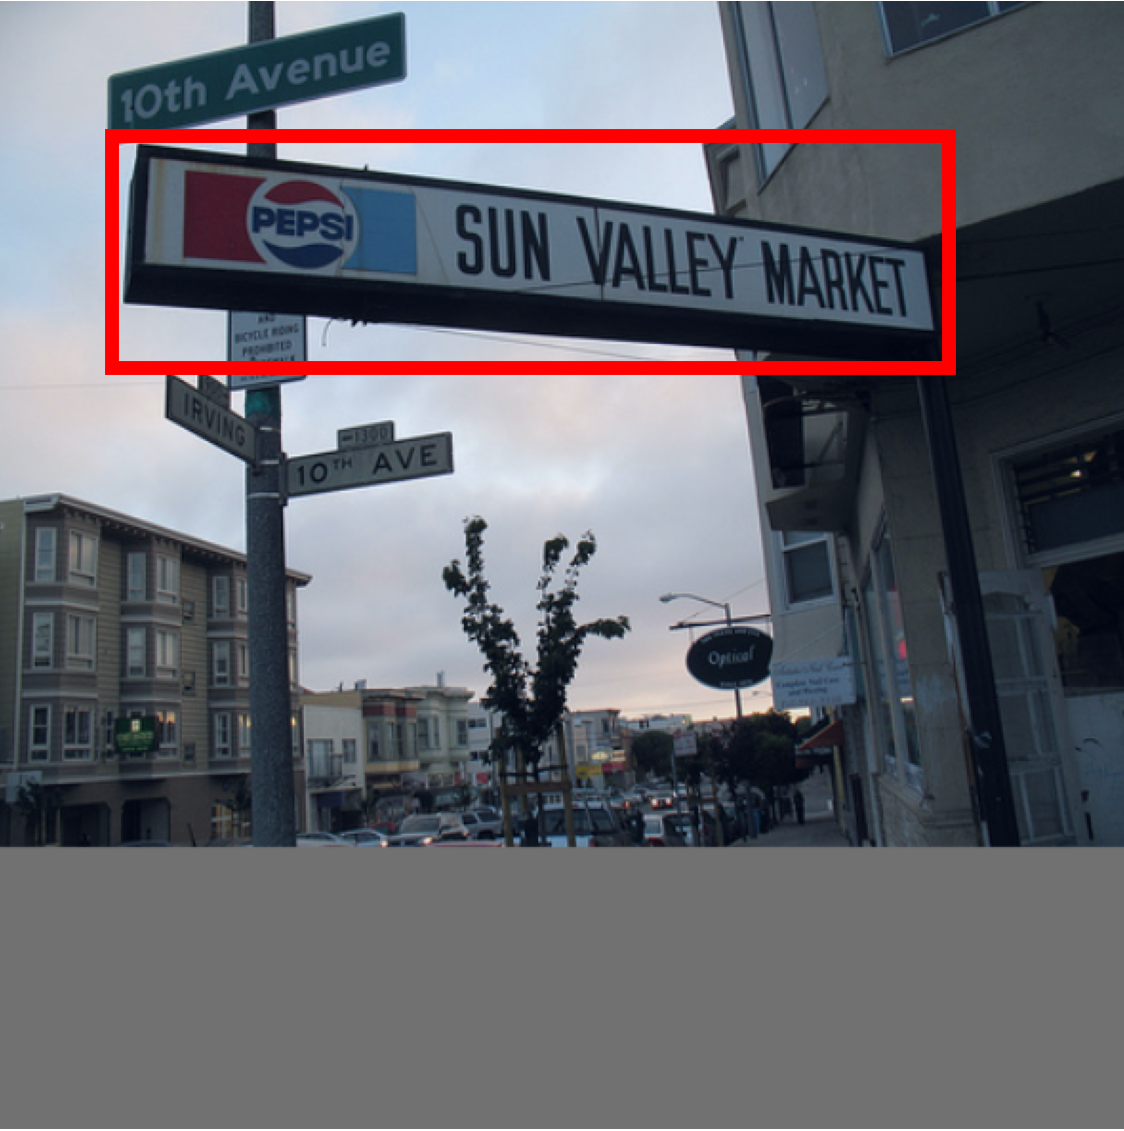
\includegraphics[width=0.9\linewidth]{figures/result/street/o3}
	\end{minipage}
		\begin{minipage}[t]{3.5cm}
			\centering
			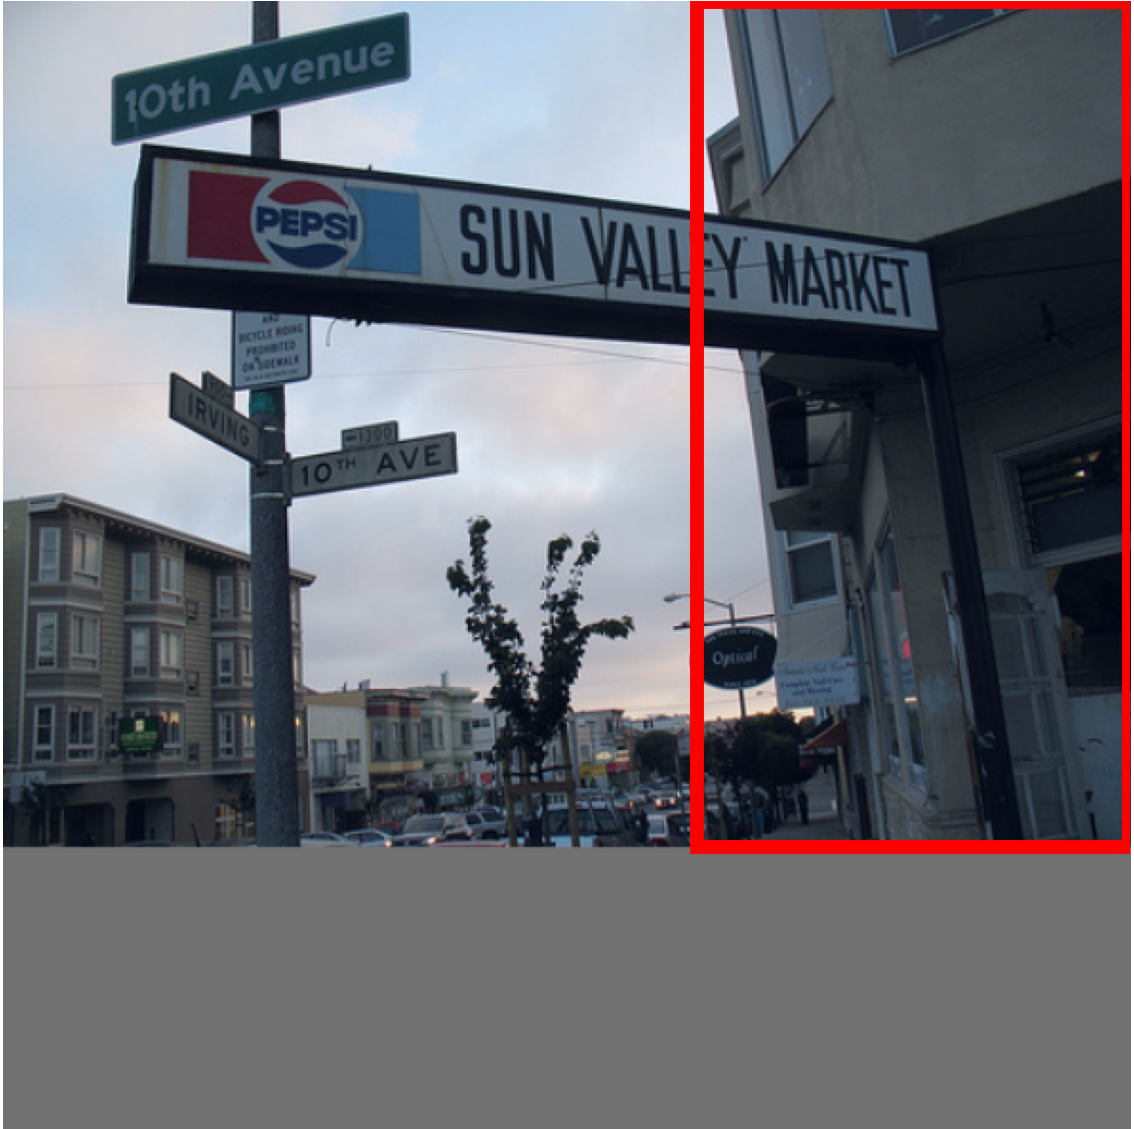
\includegraphics[width=0.9\linewidth]{figures/result/street/o4}
	\end{minipage}}
	
	\subfigure[The object query 1.]{
		\begin{minipage}[t]{3.5cm}
			\centering
			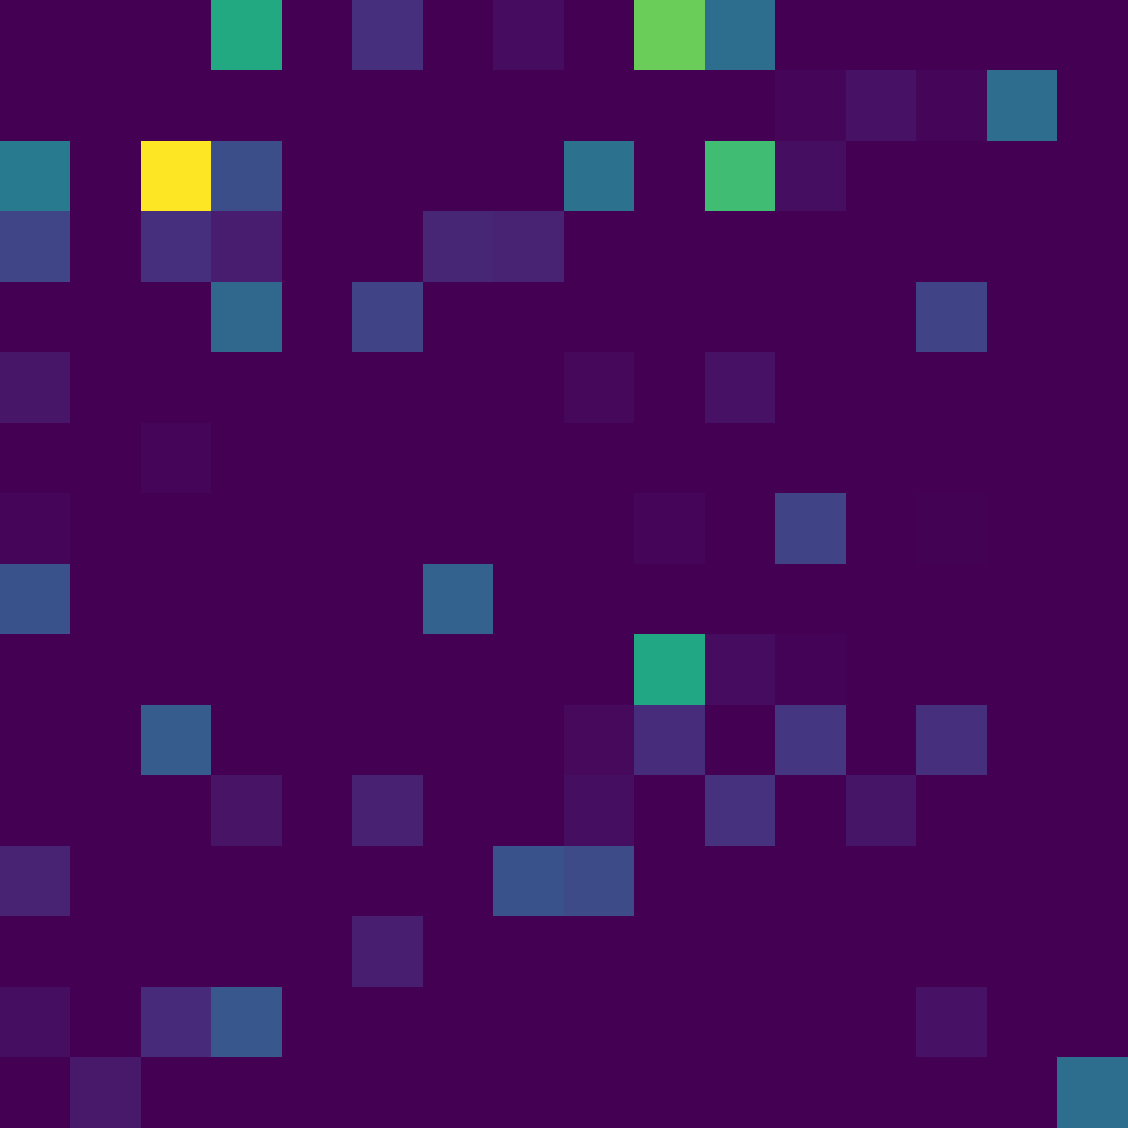
\includegraphics[width=0.9\linewidth]{figures/result/tennis/q0_2}
	\end{minipage}
		\begin{minipage}[t]{3.5cm}
			\centering
			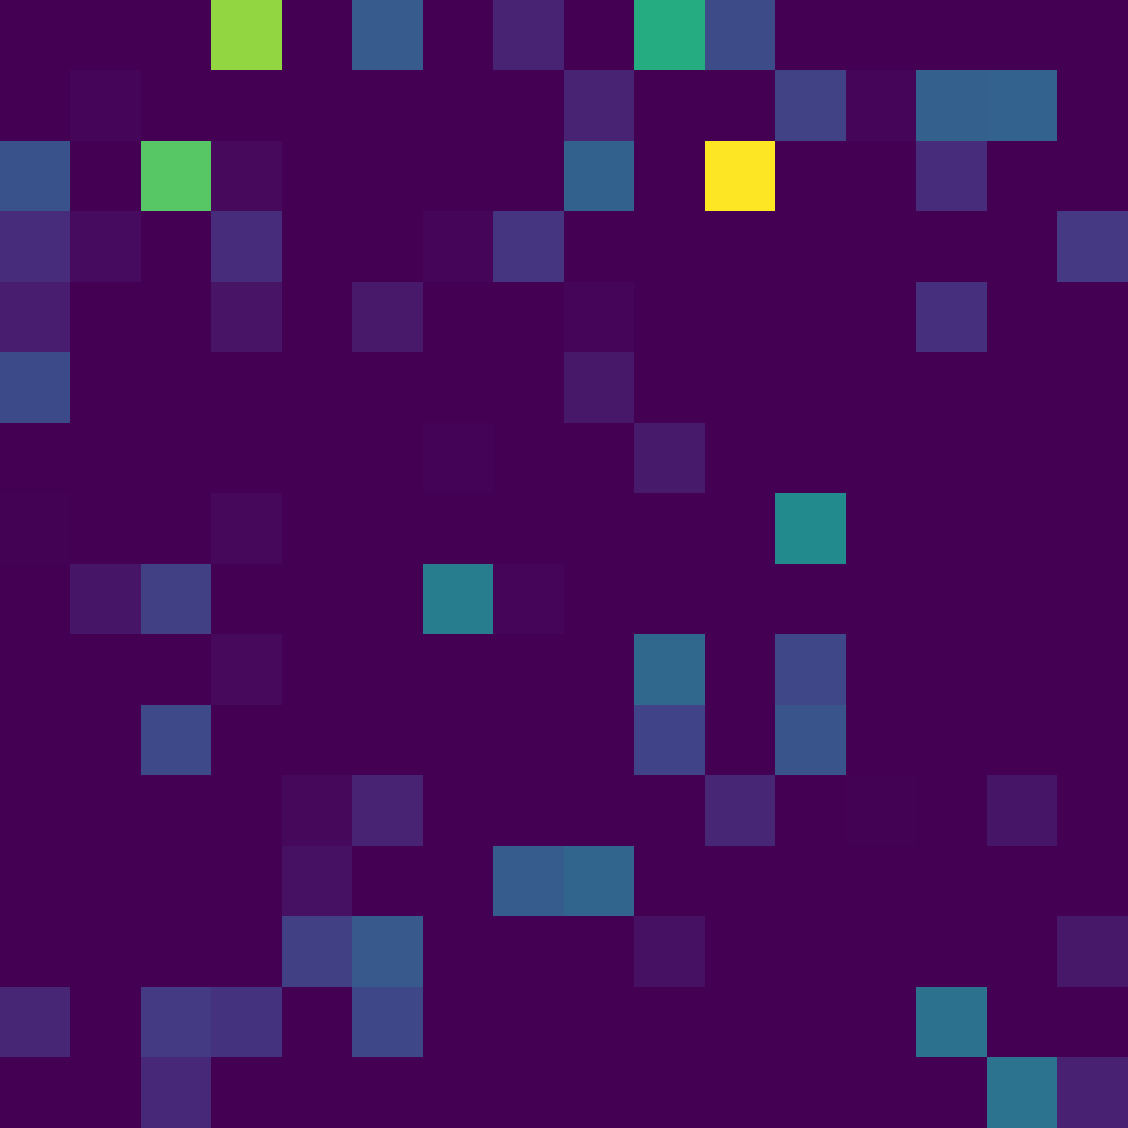
\includegraphics[width=0.9\linewidth]{figures/result/tennis/q0_4}
	\end{minipage}
	\begin{minipage}[t]{3.5cm}
		\centering
		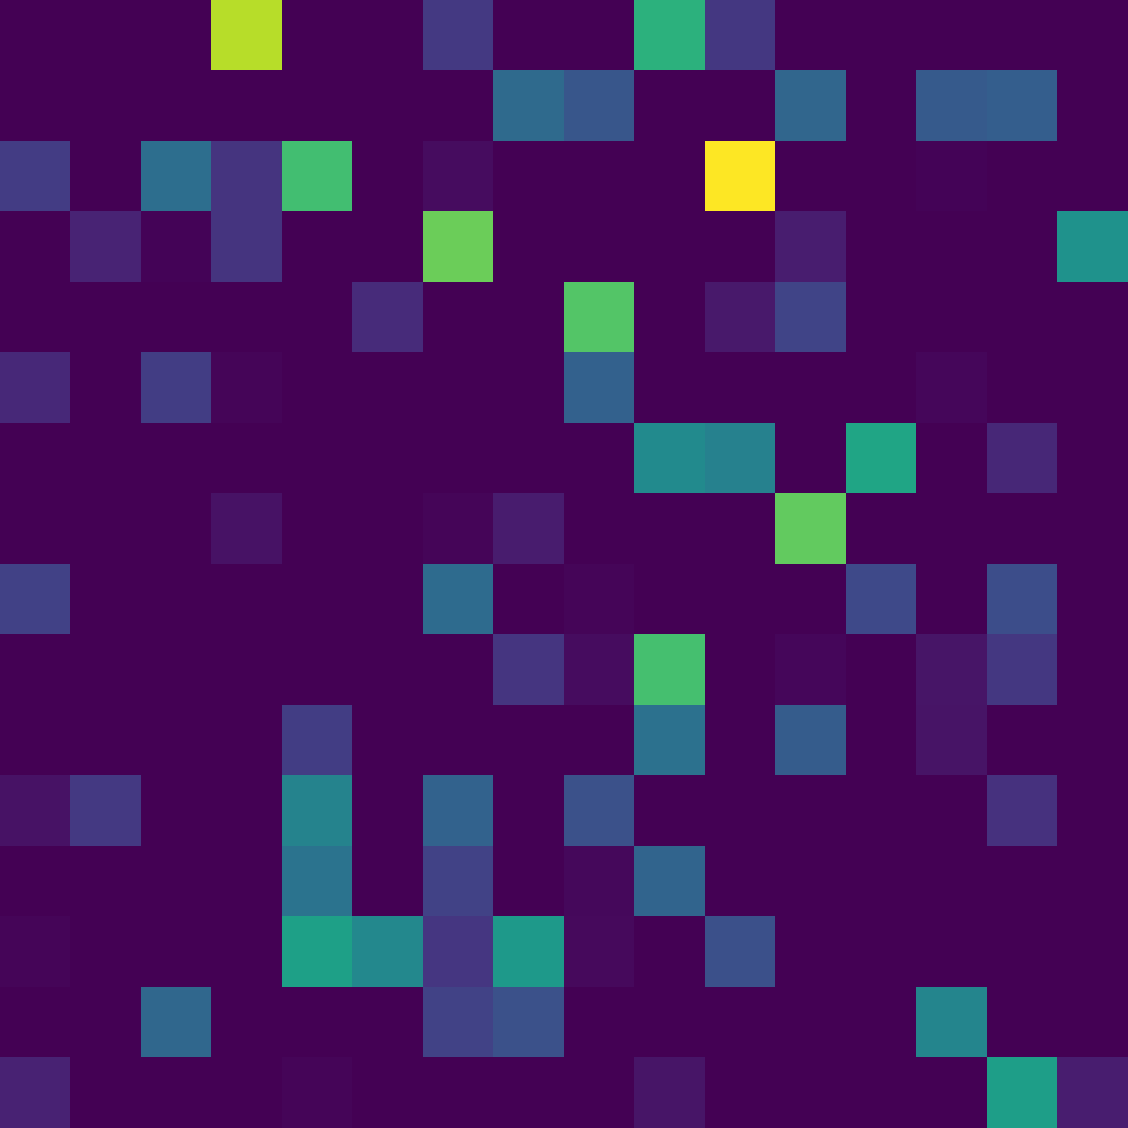
\includegraphics[width=0.9\linewidth]{figures/result/street/q0_3}
	\end{minipage}
		\begin{minipage}[t]{3.5cm}
			\centering
			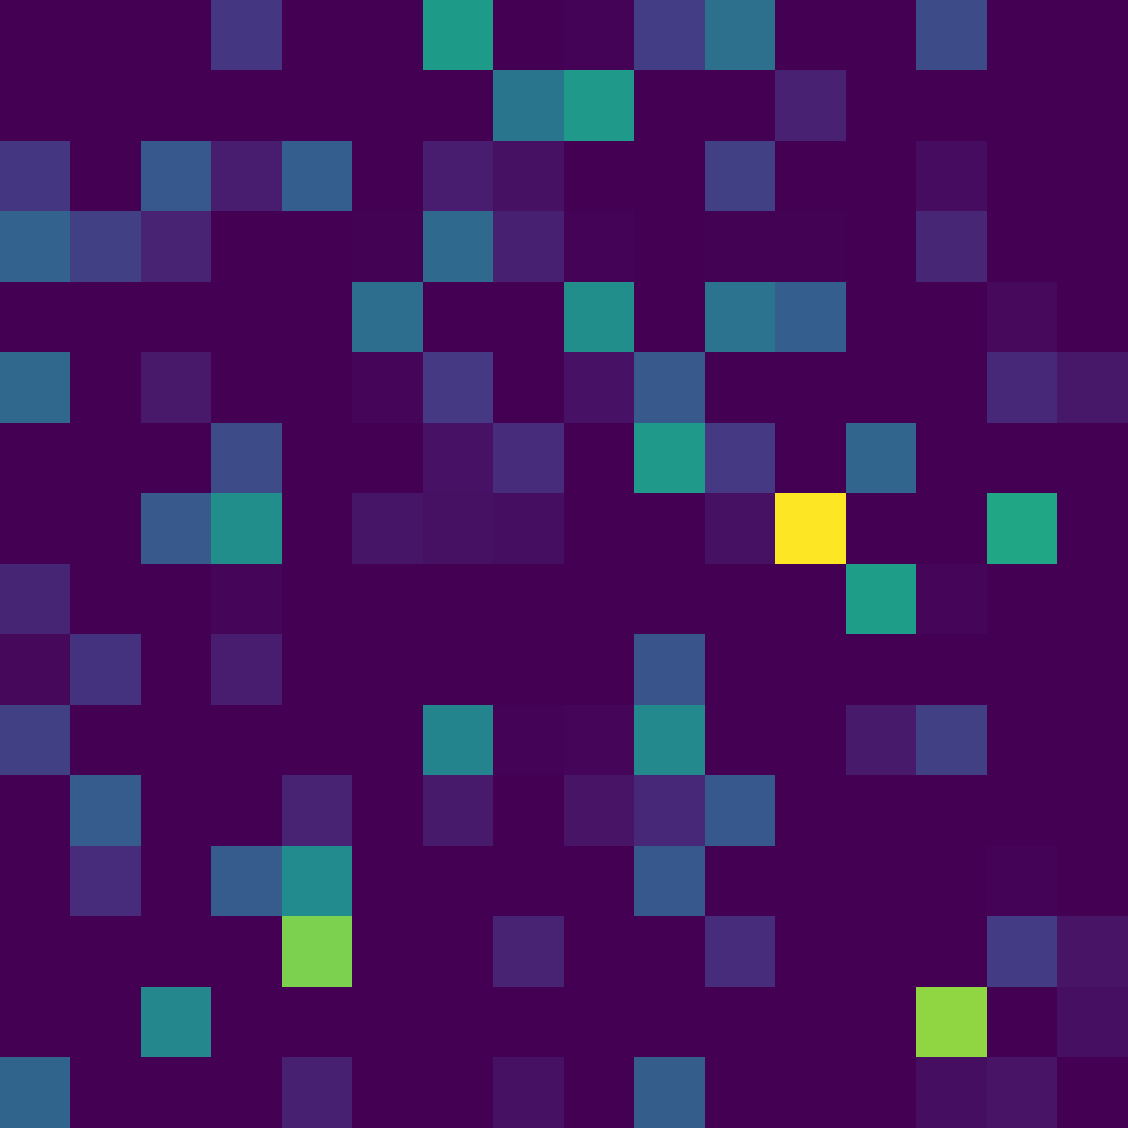
\includegraphics[width=0.9\linewidth]{figures/result/street/q0_4}
	\end{minipage}}


		\subfigure[the object query 2.]{
		\begin{minipage}[t]{3.5cm}
			\centering
			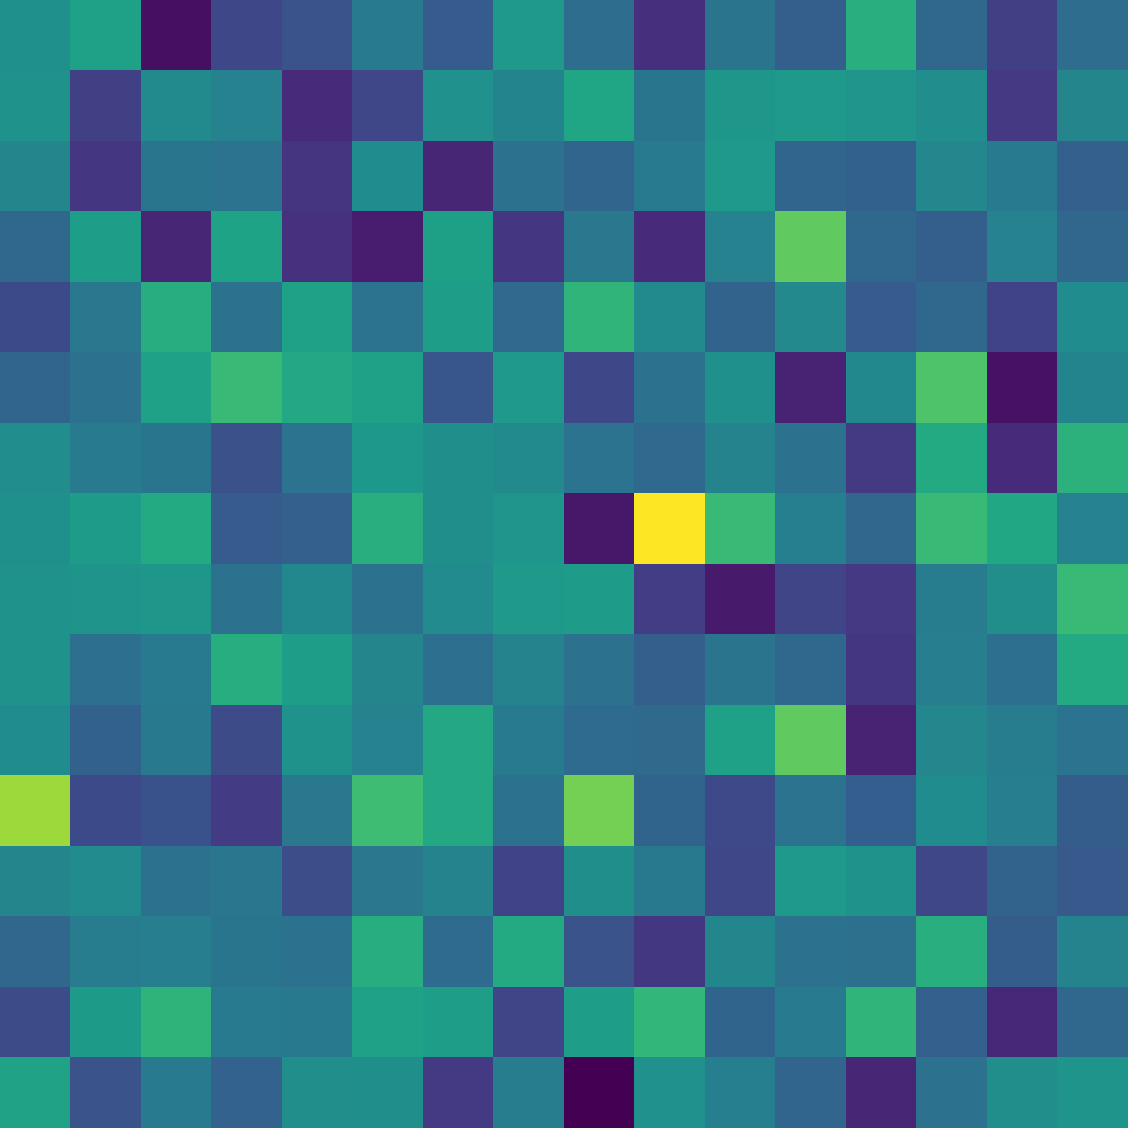
\includegraphics[width=0.9\linewidth]{figures/result/tennis/q3_2}
	\end{minipage}
		\begin{minipage}[t]{3.5cm}
			\centering
			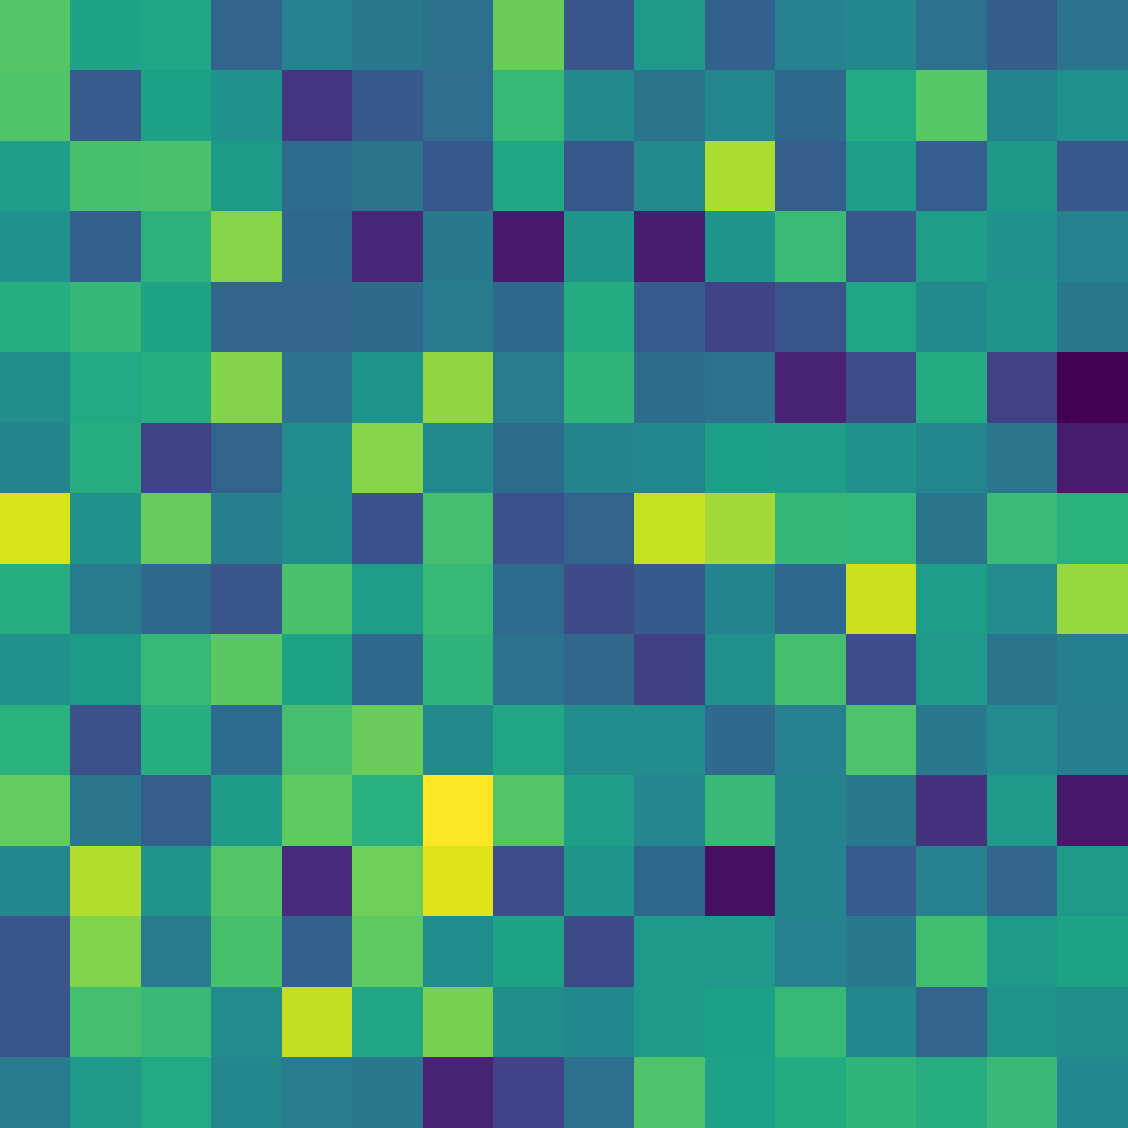
\includegraphics[width=0.9\linewidth]{figures/result/tennis/q3_4}
	\end{minipage}
		\begin{minipage}[t]{3.5cm}
			\centering
			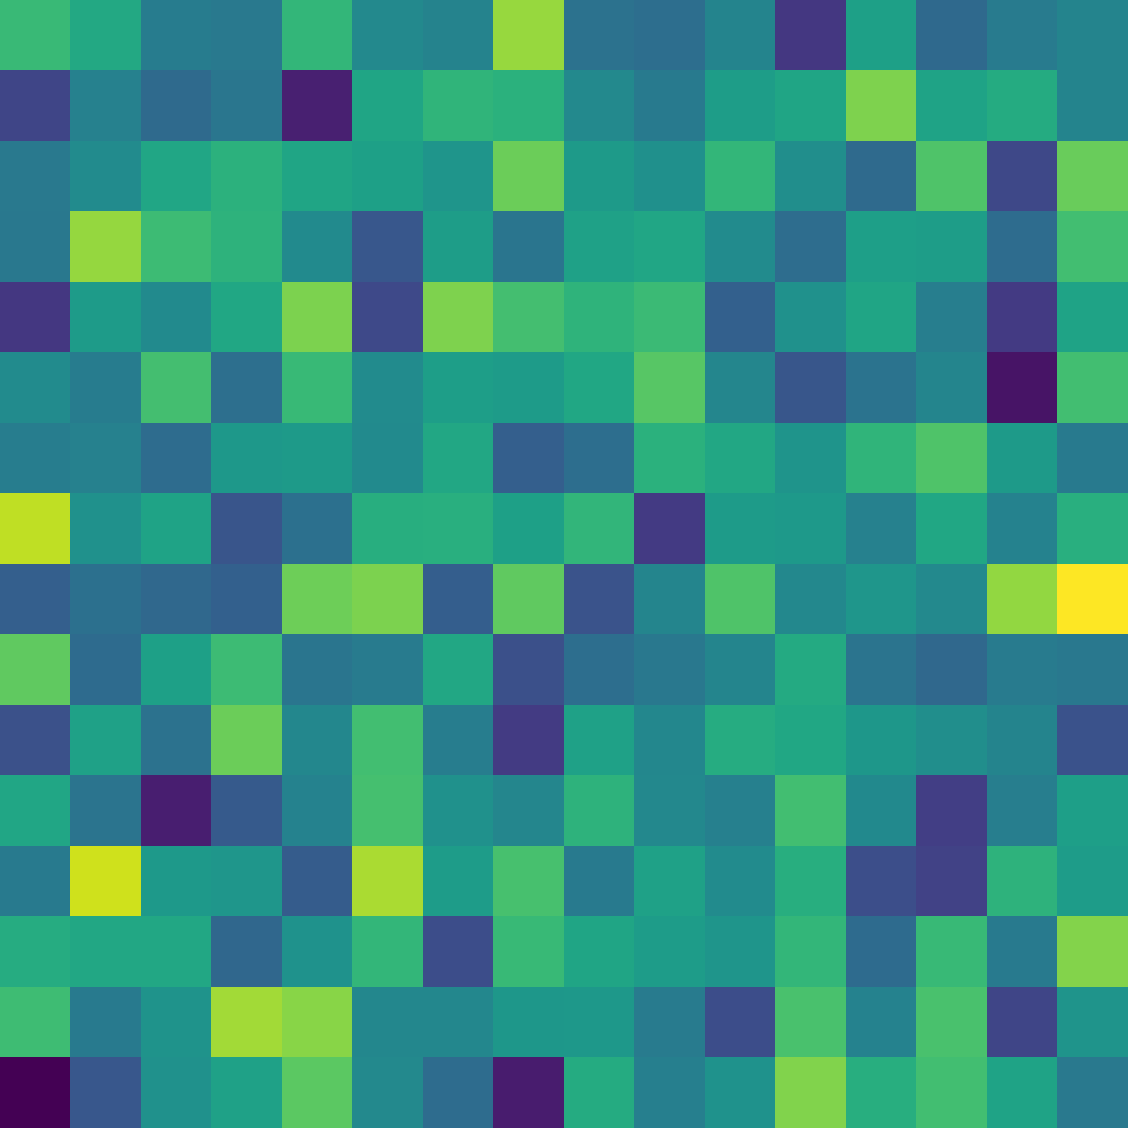
\includegraphics[width=0.9\linewidth]{figures/result/street/q3_3}
	\end{minipage}
		\begin{minipage}[t]{3.5cm}
			\centering
			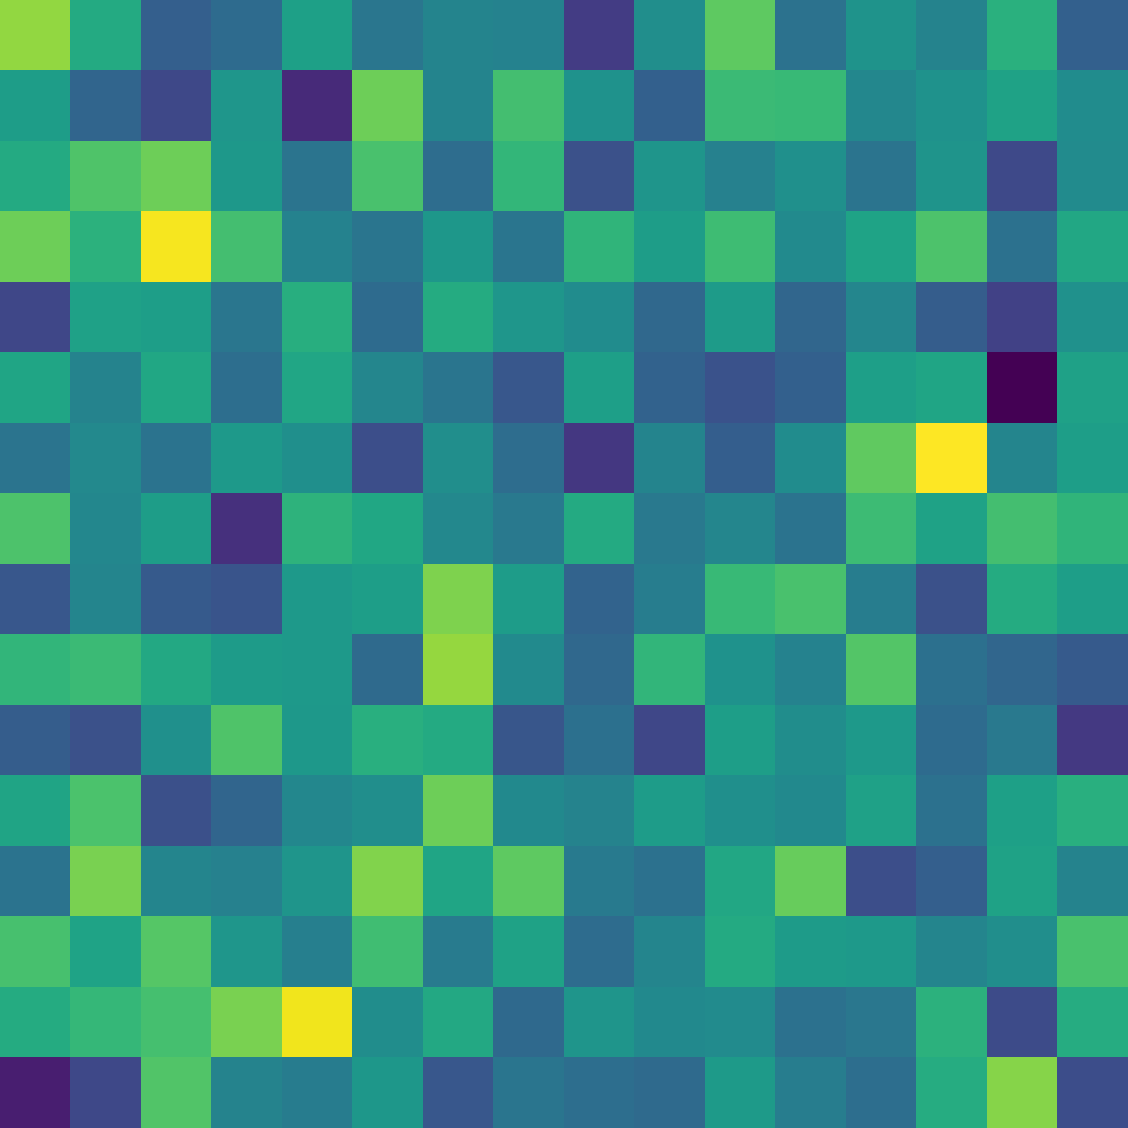
\includegraphics[width=0.9\linewidth]{figures/result/street/q3_4}
	\end{minipage}}

	\subfigure[The object query 3.]{
		\begin{minipage}[t]{3.5cm}
			\centering
			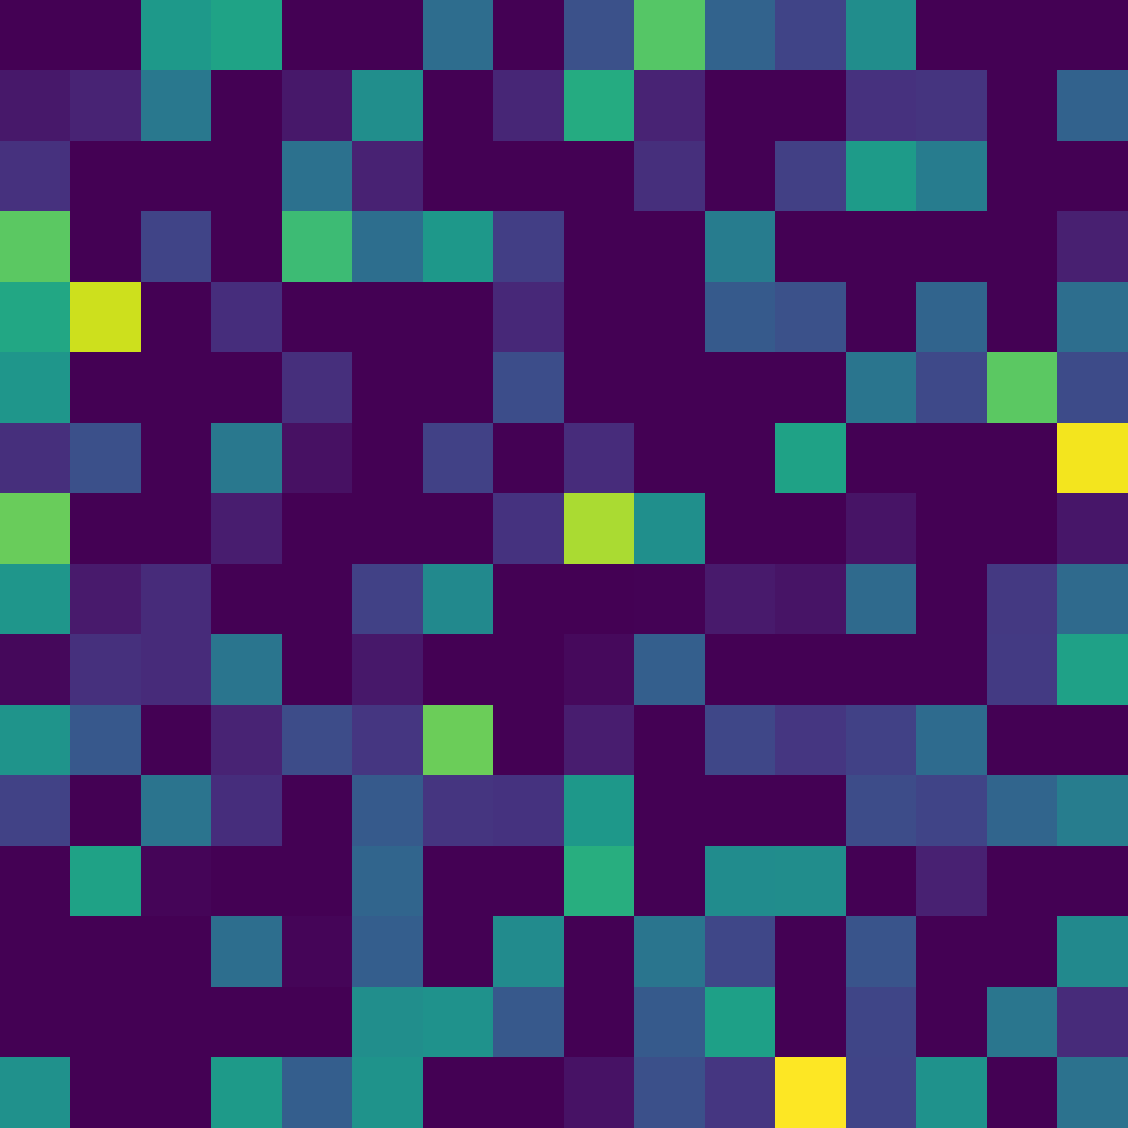
\includegraphics[width=0.9\linewidth]{figures/result/tennis/q2_2}
	\end{minipage}
		\begin{minipage}[t]{3.5cm}
			\centering
			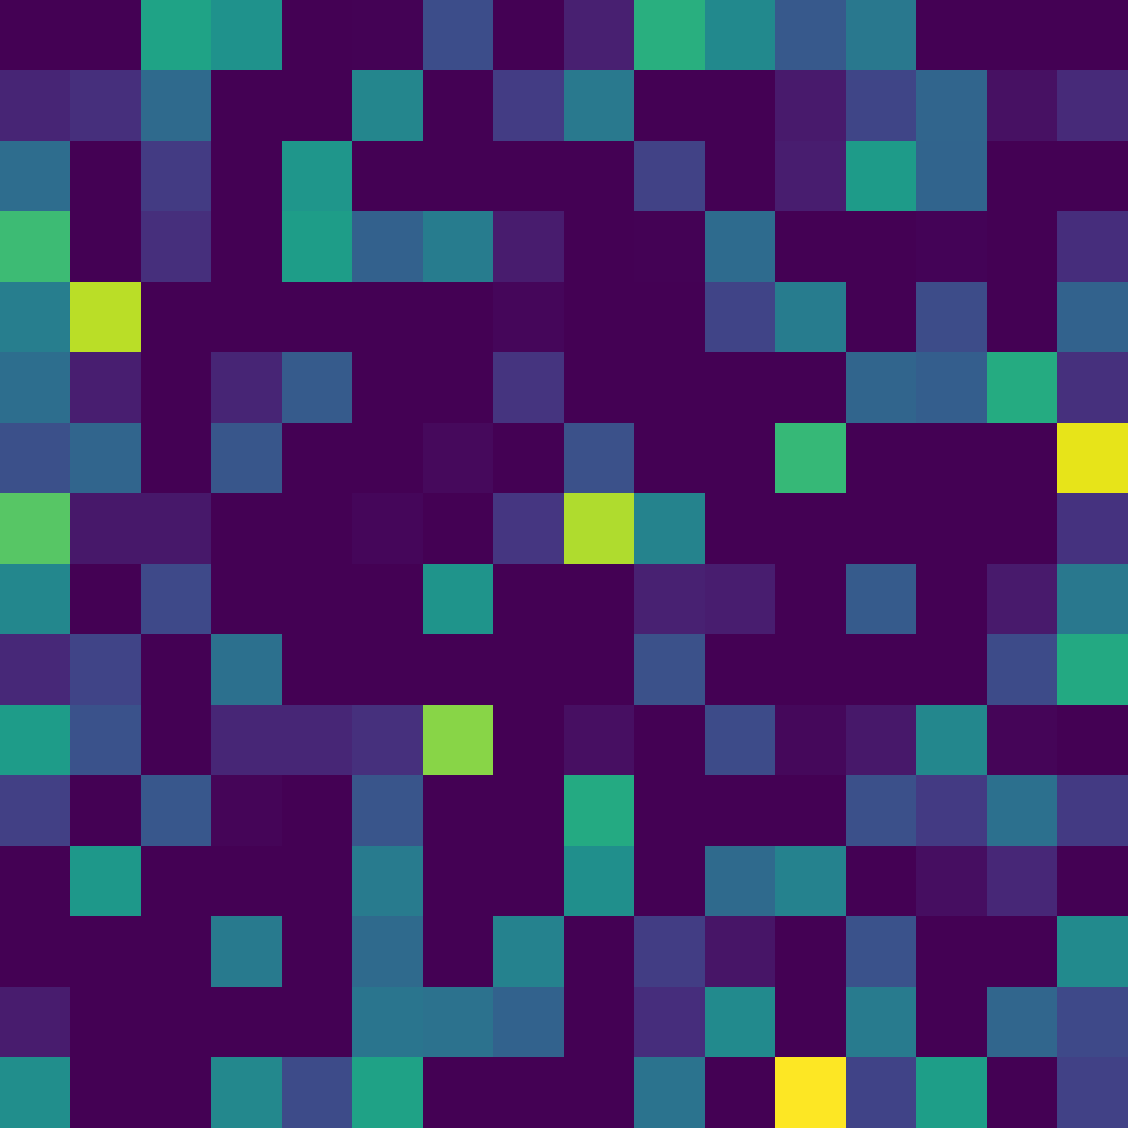
\includegraphics[width=0.9\linewidth]{figures/result/tennis/q2_4}
	\end{minipage}
	\begin{minipage}[t]{3.5cm}
	\centering
	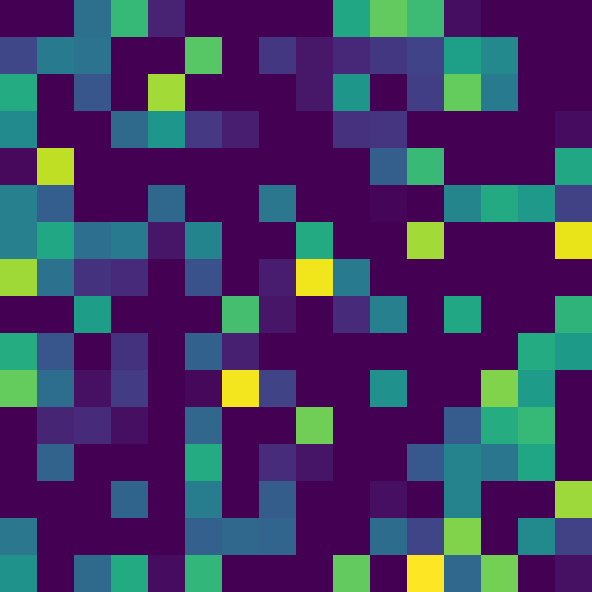
\includegraphics[width=0.9\linewidth]{figures/result/street/q2_3}
	\end{minipage}
	\begin{minipage}[t]{3.5cm}
	\centering
	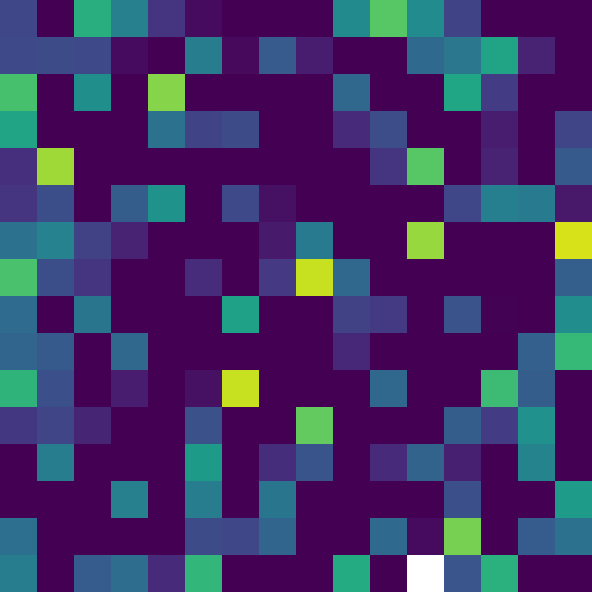
\includegraphics[width=0.9\linewidth]{figures/result/street/q2_4}
	\end{minipage}}

	\caption[An instance of Visualized results of the object query]{An instance of visualized results of the object query. From top to bottom, each row represents the position of the object, object query 1, object query 2 and object query 3.}
	\label{fig:tennis}
\end{figure}

 % 不同的object query的效果
Next, the object queries are fed into the object decoder to test their performance in the PredCLS, and recall@50 and recall@100 as the evaluation metrics. The results are in Table~\ref{tab:result_object _query}.

\begin{table}[!h]
	\centering
	\begin{tabular}{c|ccc}
		\hline
		& object query 1 & object query 2 & object query 2 \\ \hline
		Recall@50  & 62.9            & 63.2            & 63.0              \\
		Recall@100 & 65.0             & 65.3              & 65.1              \\ \hline
	\end{tabular}

\caption[The comparison of the object queries in PredCLS]{The comparison of the object queries in PredCLS.}
\label{tab:result_object _query}
\end{table}

According to the above table,  the conclusions as follows:

\begin{enumerate}
	\item The object query and object feature we designed correspond to each other, which can replace learnable query and solve the VRD problem.
	\item The performance of the three object queries in PredCLS is similar. So it only need to design a query that can distinguish objects, that is, each query needs to correspond to a unique entity. 
\end{enumerate}

\subsubsection{Experiment on Object Context}
In order to obtain more information that is conducive to predicate prediction, the object context is designed to obtain the interaction between objects. It contains a global context of an object to all objects. Predicate prediction itself is to detect the interaction between objects, so a context that can indicate the interaction information between them is very necessary. Remove $ context_{obj }$ in the predicate classifier and compare the formula ~\ref{equ:predicatd}  and ~\ref{equ:predicatc} to detect the effect of object context on Predicate Classification.
% 为了获取更多有利于谓语预测的信息,我们设计了object context,去获得object 之间的交互,它包含了一个object 对所有object的上下文关系。谓语预测本身就是检测object间的交互,所以一个能表明他们之间的交互信息的context是十分必要的。在predicate classifier中去掉 $ context_{obj }$ 使用如下公式~\ref{equ:predicatd}与公式~\ref{equ:predicatc}进行对比,检测object  context 对Predicate Classification的作用效果。

\begin{equation}
	score'_{pred}(i,j) = Linear(concat(feat_{obj}^i, context_{rel}^{ij}, feat_{obj}^j)
	\label{equ:predicatd}
\end{equation}

\begin{table}[]
	\begin{tabular}{llll}
		\hline
		a & sd & dw  & asd \\ \hline
		3 & 12 & 231 & 12  \\ \hline
	\end{tabular}
\end{table}

\begin{table}[]
	\centering
	\begin{tabular}{c|lcc}
		\hline
		\multirow{2}{*}{}      & \multicolumn{3}{l}{Predicate Classification}  \\ \cline{2-4} 
		& R@20          & R@50          & R@100         \\ \hline
		without object context & 51.7          & 59.6          & 62.3          \\
		with object context    & \textbf{55.4} & \textbf{63.4} & \textbf{64.4} \\ \hline
	\end{tabular}
\caption[The impact of object context on PredCLS]{The impact of object context on PredCLS.}
\label{tab:object context}
\end{table}
As shown in Table~\ref{tab:object context}, the object context has great benefits for the predicate prediction, especially the improvement of recall@20 is the most obvious, with an improvement of 3.7. This verifies the effect of global context between objects on predicate prediction.% 通过上表,可是肯定object context 对谓语预测的有很大帮助,尤其是recall@20的提高最为明显,有3.7的提升。这验证的global context between objects 对谓语预测的作用。

\subsection{Experiment on Attention  Loss Function}

An attention loss is designed to make the object feature better and some experiments are performed to verify it.

The Figure~\ref{fig:attention_loss_result} is the training result of the attention loss. We record a loss every 100 steps, summing up 1000 data, and use Matlab to perform low-pass filtering to draw the result. It is showed that the attention from the beginning $ 10^{-4} $ dropped rapidly and gradually tended to 0 after 500 steps.

In the object decoder in our model in Fig.~\ref{fig:objectdecoder}, when the feature of the object is obtained, it will be accompanied by the corresponding attention map. Its size is $ 64\times1369 $, corresponding to each object, it is reshaped into a size of $ 37\times37 $ object attention map. As shown in Fig.~\ref{fig:train_attention_loss} and Fig.~\ref{fig:bus}. The first and second image are selected in our test data set, and the object bounding boxes and their attention maps (with and without attention loss) are drawn.

\begin{figure}[H]
	\centering
	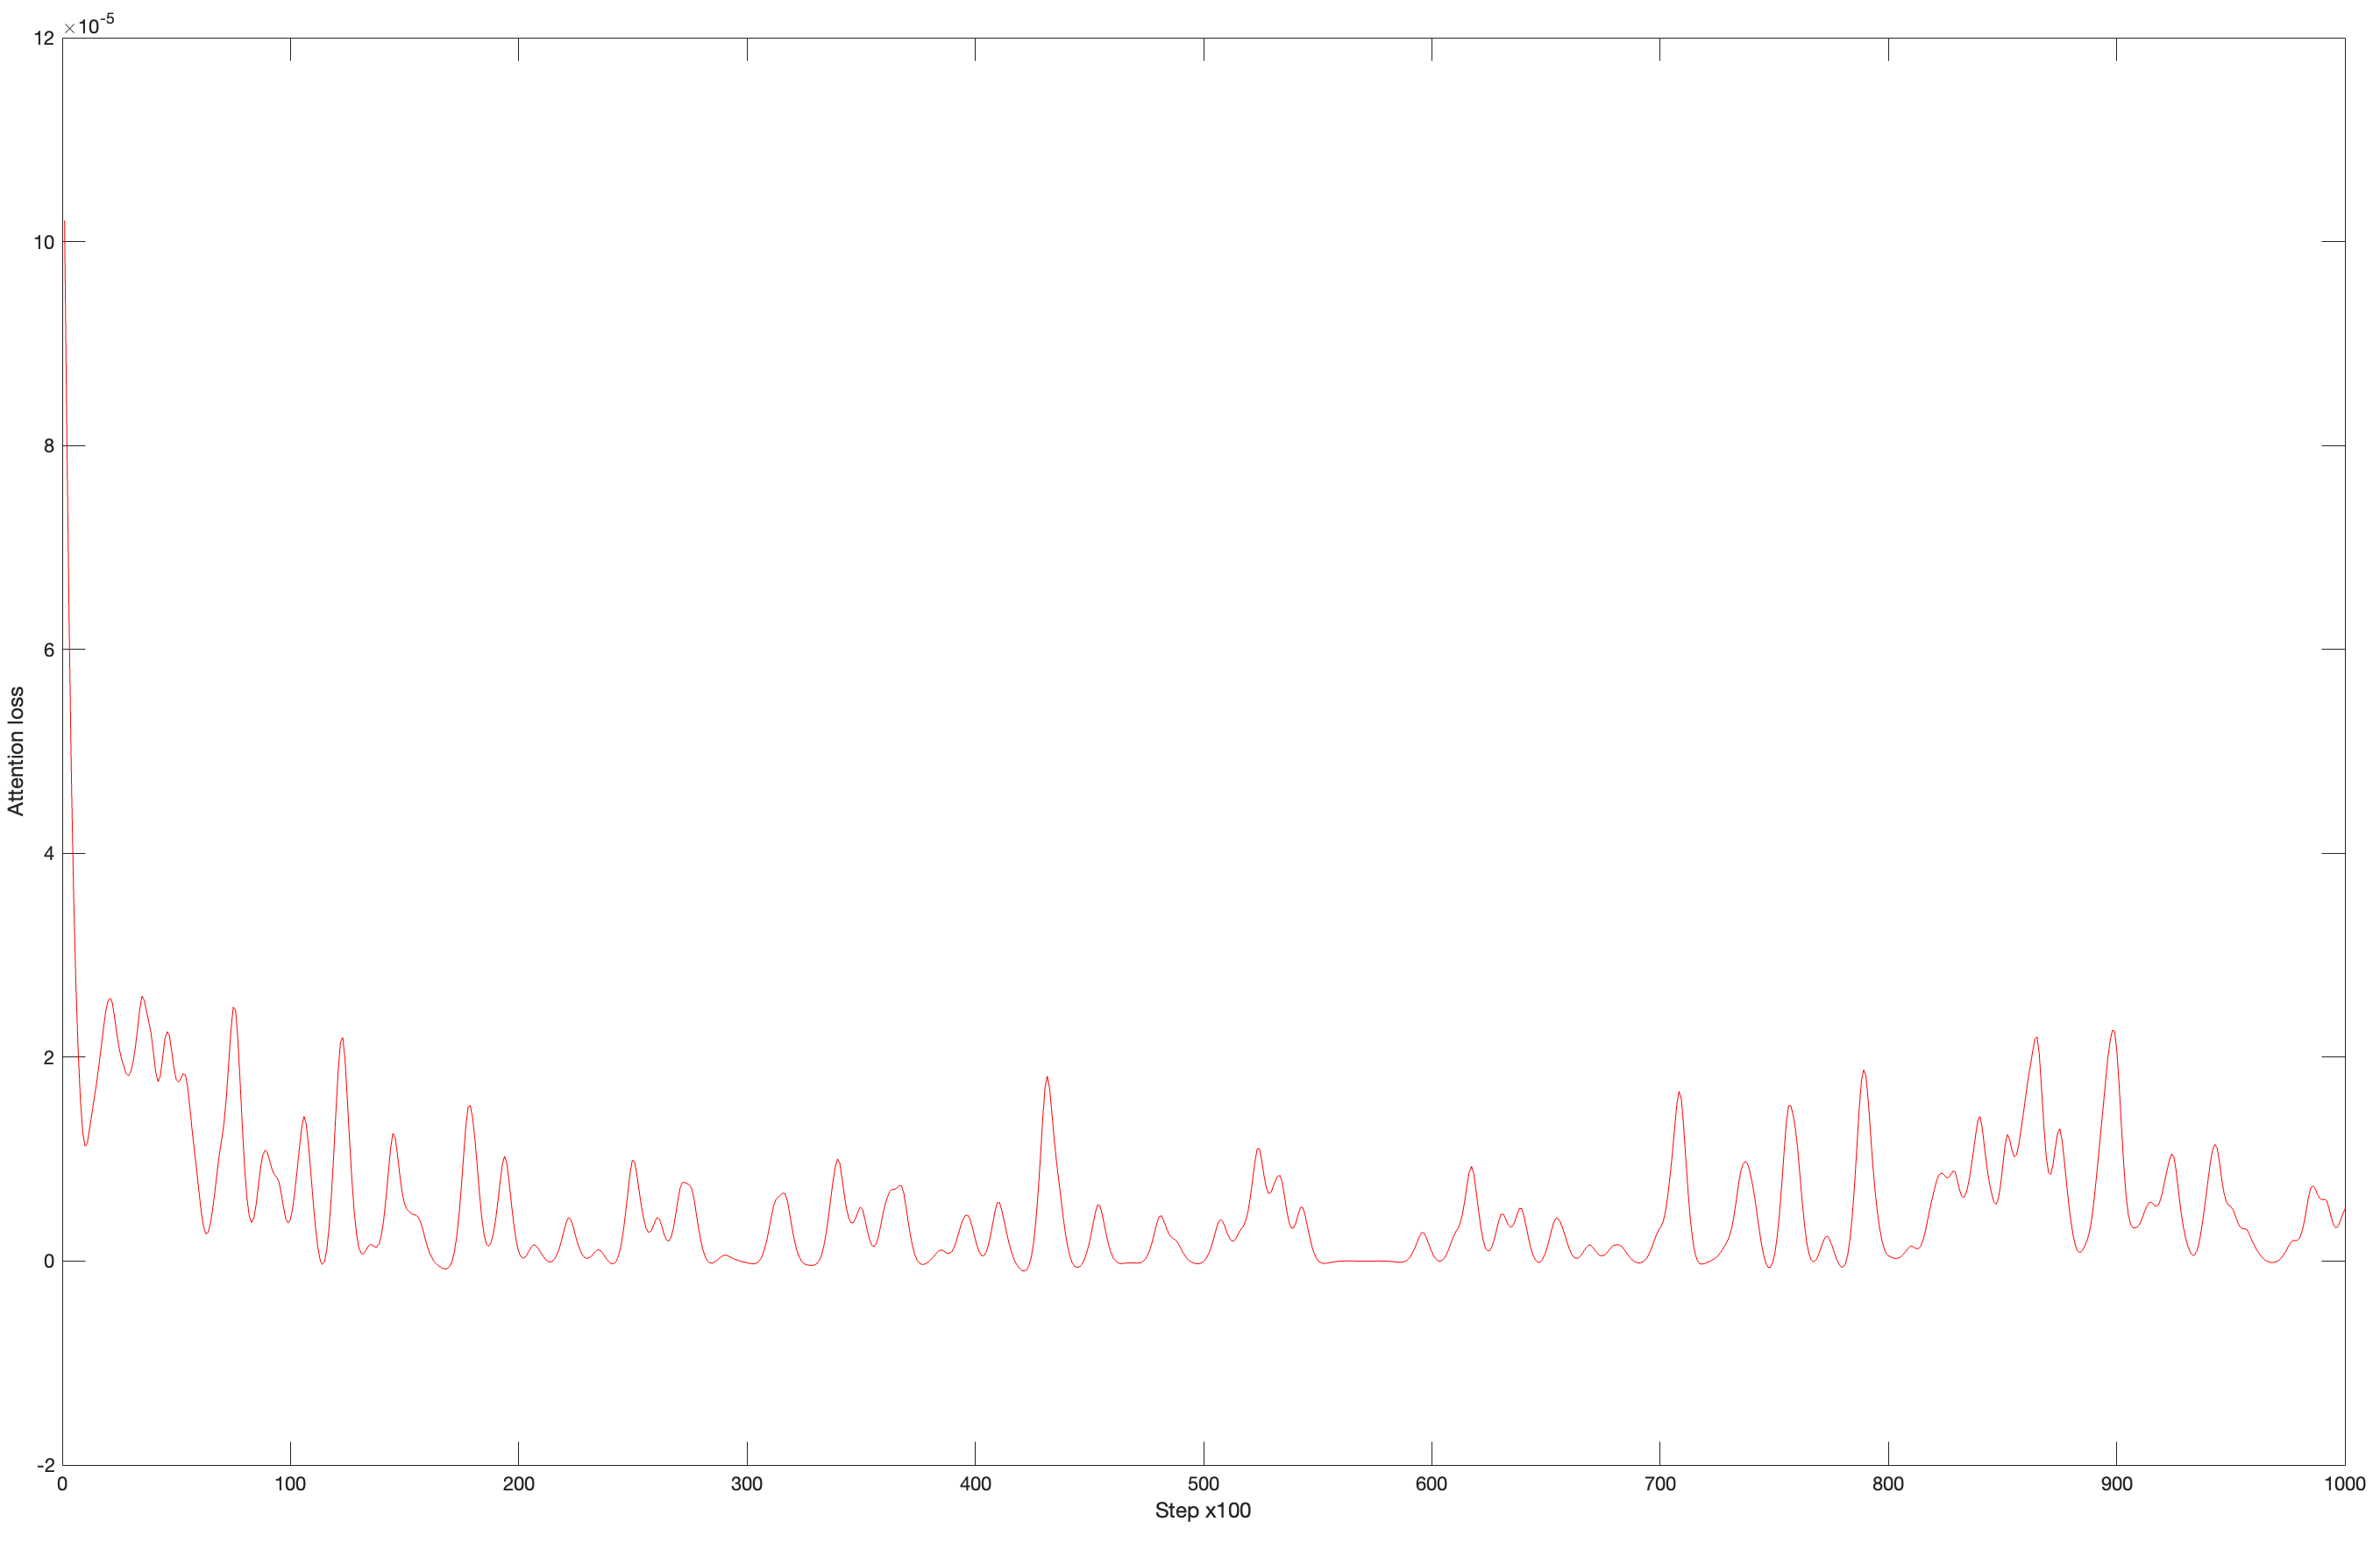
\includegraphics[width=0.7\linewidth]{figures/result/attention_loss}
	\caption[Training result of the Attention Loss]{Training result of the Attention Loss.}
	\label{fig:attention_loss_result}
\end{figure}

It can be seen that the attention loss performs successfully on the attention map. Without attention loss, the attention map is messy. As shown in Fig.~\ref{fig:train_attention_loss}(b), the position and shape of the train can be distinguished well in the attention map, and it even express the position of the train better than the bounding box. The background area of the picture is blue, and the background color in the picture is very uniform, which makes the attention weight of the object very obvious. It means the object decoder pays more attention to this object.

\begin{figure}[H]
	\centering
	\subfigure[train]{
		\begin{minipage}[t]{5cm}
			\centering
			\includegraphics[width=0.9\linewidth]{figures/result/train/obj1}
	\end{minipage}}
	\subfigure[attention map with our loss]{
		\begin{minipage}[t]{5cm}
			\centering
			\includegraphics[width=0.9\linewidth]{figures/result/train/att1}
	\end{minipage}}
	\subfigure[ attention map without our loss]{
		\begin{minipage}[t]{5cm}
			\centering
			\includegraphics[width=0.9\linewidth]{figures/result/train/no1}
	\end{minipage}}
	
	\subfigure[haus]{
		\begin{minipage}[t]{5cm}
			\centering
			\includegraphics[width=0.9\linewidth]{figures/result/train/obj2}
	\end{minipage}}
	\subfigure[attention map with our loss]{
		\begin{minipage}[t]{5cm}
			\centering
			\includegraphics[width=0.9\linewidth]{figures/result/train/att2}
	\end{minipage}}
	\subfigure[attention map without our loss]{
		\begin{minipage}[t]{5cm}
			\centering
			\includegraphics[width=0.9\linewidth]{figures/result/train/no2}
	\end{minipage}}
	
	\subfigure[man]{
		\begin{minipage}[t]{5cm}
			\centering
			\includegraphics[width=0.9\linewidth]{figures/result/train/obj3}
	\end{minipage}}
	\subfigure[attention map with our loss]{
		\begin{minipage}[t]{5cm}
			\centering
			\includegraphics[width=0.9\linewidth]{figures/result/train/att3}
	\end{minipage}}
	\subfigure[attention map without our loss]{
		\begin{minipage}[t]{5cm}
			\centering
			\includegraphics[width=0.9\linewidth]{figures/result/train/no3}
	\end{minipage}}
	
	\subfigure[window]{
		\begin{minipage}[t]{5cm}
			\centering
			\includegraphics[width=0.9\linewidth]{figures/result/train/obj4}
	\end{minipage}}
	\subfigure[attention map with our  loss]{
		\begin{minipage}[t]{5cm}
			\centering
			\includegraphics[width=0.9\linewidth]{figures/result/train/att4}
	\end{minipage}}
	\subfigure[attention map without our loss]{
		\begin{minipage}[t]{5cm}
			\centering
			\includegraphics[width=0.9\linewidth]{figures/result/train/no4}
	\end{minipage}}
	
	\caption[The visualization of our attention loss of the first image in the test dataset]{The visualization of our attention loss of the first image in the test dataset. The first column is the object bounding box, the second column is the visualization result of the attention map when we use the attention loss, and the third column is the visualization result of the attention map without our attention loss.}
	\label{fig:train_attention_loss}
\end{figure}




\begin{figure}[H]
	\centering
	\subfigure[bus]{
		\begin{minipage}[t]{5cm}
			\centering
			\includegraphics[width=0.9\linewidth]{figures/result/bus/obj1}
	\end{minipage}}
	\subfigure[attention map with our loss]{
		\begin{minipage}[t]{5cm}
			\centering
			\includegraphics[width=0.9\linewidth]{figures/result/bus/att1}
	\end{minipage}}
	\subfigure[attention map without our loss]{
		\begin{minipage}[t]{5cm}
			\centering
			\includegraphics[width=0.9\linewidth]{figures/result/bus/no1}
	\end{minipage}}
	
	\subfigure[man]{
		\begin{minipage}[t]{5cm}
			\centering
			\includegraphics[width=0.9\linewidth]{figures/result/bus/obj2}
	\end{minipage}}
	\subfigure[attention map with our loss]{
		\begin{minipage}[t]{5cm}
			\centering
			\includegraphics[width=0.9\linewidth]{figures/result/bus/att2}
	\end{minipage}}
	\subfigure[attention map without our loss]{
		\begin{minipage}[t]{5cm}
			\centering
			\includegraphics[width=0.9\linewidth]{figures/result/bus/no2}
	\end{minipage}}
	
	\subfigure[pants]{
		\begin{minipage}[t]{5cm}
			\centering
			\includegraphics[width=0.9\linewidth]{figures/result/bus/obj3}
	\end{minipage}}
	\subfigure[ attention map with our loss]{
		\begin{minipage}[t]{5cm}
			\centering
			\includegraphics[width=0.9\linewidth]{figures/result/bus/att3}
	\end{minipage}}
	\subfigure[ attention map without our loss]{
		\begin{minipage}[t]{5cm}
			\centering
			\includegraphics[width=0.9\linewidth]{figures/result/bus/no3}
	\end{minipage}}
	
	\subfigure[board]{
		\begin{minipage}[t]{5cm}
			\centering
			\includegraphics[width=0.9\linewidth]{figures/result/bus/obj4}
	\end{minipage}}
	\subfigure[ attention map with our loss]{
		\begin{minipage}[t]{5cm}
			\centering
			\includegraphics[width=0.9\linewidth]{figures/result/bus/att4}
	\end{minipage}}
	\subfigure[ attention map without our loss]{
		\begin{minipage}[t]{5cm}
			\centering
			\includegraphics[width=0.9\linewidth]{figures/result/bus/no4}
	\end{minipage}}
	
	\caption[The visualization of our attention loss of the second image in the test dataset]{The visualization of our attention loss of the second image in the test dataset. The first column is the object bounding box, the second column is the visualization result of the attention map when we use the attention loss, and the third column is the visualization result of the attention map without our attention loss.}
	\label{fig:bus}
\end{figure}


\begin{table}[!h]
	\centering
	\begin{tabular}{c|ccc|ccc}
		\hline
		\multirow{2}{*}{}           & \multicolumn{3}{c|}{PredCLS} & \multicolumn{3}{c}{SGCLS} \\ \cline{2-7} 
		& R@20    & R@50    & R@100    & R@20   & R@50   & R@100   \\ \hline
		without our attention  loss & 53.9      & 61.8       & 64.0       & 25.7     & 30.7     & 31.4   \\
		with our attention loss     & \textbf{55.4}       & \textbf{63.3}       & \textbf{65.2 }       & \textbf{28.4 }     & \textbf{32.7}      &\textbf{33.6}     \\ \hline
	\end{tabular}
	
	\caption[The result of attention loss in PredCLS and SGCLS]{The result of attention loss in PredCLS and SGCLS.}
	\label{tab:result_attetnion_loss}
\end{table}


According to Table~\ref{tab:result_attetnion_loss}, in PredCLS R@50 has an improvement of about 0.1, and in SGCLS it is even greater by about 0.2.

Based on the above results, the conclusion is as follows  :
\begin{enumerate}
	\item Our attention loss can effectively change the attention map so that it can be well visualized and can show the position and shape of each object.
	\item Our attention loss can get a better object feature, so as to better solve the VRD problem.
\end{enumerate}

\subsection{Experiment on Relation Deocder}
In this section,  experiments on the relation decoder are conducted. Based on the results of the previous object query, a different relation query is designed, and it makes our relation context have the spatial information and semantic information of the object.

%In Figure~\ref{fig:relation_d_vis}, we can see that the relationship query we designed has differences between each relationship pair. For example, in the figure (a) represents pair $ <man, pants?>$ and (b) represents pair $ <pant, man> $, their subject and The objects are opposite, but their relations are different. In the figure (c) is relation pair $ <man1, glove> $ and d is $ <man1, man2> $. They have the same subject and different objects, but their relation queries are also significantly different.

In Figure~\ref{fig:relation_attetnion}, the context effect is expressed through attention between relation and object. When the relational context is obtained through the relational decoder, it will be accompanied by an attention map. The sub-figure(c) and (f) are attention map, which y-axis represents the relation pair and its x-axis represents the object. Our relation pair contains both ground truth pair and no relation pair. For example, in sub-figure(a), the ground truth pair $<glass, table> $ has higher attention weight for object \textit{`glass'} and \textit{`table'} than others, which means that this pair pays more attention to the objects \textit{`glass'} and \textit{`table'}. No relation pair has the same effect. For example, in the attention map on the right,the attention values of the object \textit{ `hair'} and \textit{`glove'} in the pair $<hair, glove> $   is higher than the object \textit{`girl'}.


\begin{figure}[!htp]
	\centering
	\subfigure[Scene graph]{
		\begin{minipage}[t]{5cm}
			\centering
			\includegraphics[width=0.7\linewidth]{figures/result/relation_Attention/img1}
		\end{minipage}}
	\subfigure[Ground truth relationships ]{
		\begin{minipage}[t]{5cm}
			\centering
			\includegraphics[width=0.8\linewidth]{figures/result/relation_Attention/rel1}
		\end{minipage}}
	\subfigure[Attention map]{
		\begin{minipage}[t]{5cm}
			\centering
			\includegraphics[width=1\linewidth]{figures/result/relation_Attention/att1}
	\end{minipage}}
	
	\subfigure[Scene graph]{
		\begin{minipage}[t]{5cm}
			\centering
			\includegraphics[width=0.7\linewidth]{figures/result/relation_Attention/img2}
		\end{minipage}}
	\subfigure[Ground truth relationships]{
		\begin{minipage}[t]{5cm}
			\centering
			\includegraphics[width=0.35\linewidth]{figures/result/relation_Attention/rel2}
		\end{minipage}}
	\subfigure[Attention map]{
		\begin{minipage}[t]{5cm}
			\centering
			\includegraphics[width=1\linewidth]{figures/result/relation_Attention/att2}
		\end{minipage}
	}
	
	\caption[The visualized results of the relation decoder attention.]{The visualized results of the relation decoder attention. We get the attention map from the second attention module of the relation decoder, it means which objects the relation pair pays more attention to, and the corresponding  attention weight will be higher in this map.}
	\label{fig:relation_attetnion}
\end{figure}

The Table~\ref{tab:result_relation_decoder} is the result of using the relation decoder in the PredCLS. It shows that the relation decoder is very helpful to solve the VRD problem, and the effect is remarkable.

\begin{table}[!h]
	\centering
	\begin{tabular}{c|ccc}
		\bottomrule
		& R@20    & R@50    & R@100      \\ \hline
		without our relation decoder  & 51.1    &58.7      & 61.1    \\
		with our relation decoder      & \textbf{55.67} & \textbf{63.40} & \textbf{65.41}     \\ \bottomrule
	\end{tabular}
	
	\caption[The result of our relation decoder in PredCLS]{The result of our relation decoder in PredCLS.}
	\label{tab:result_relation_decoder}
\end{table}

In Relation Decoder, visual features, spatial features and semantic features are used to express objects, see Figure~\ref{fig:relationdecoder}. In order to verify how to express object features to achieve the best experimental results, the following experiments are conducted:

The visual feature is extracted from the image visual feature by the object decoder, and the spatial feature is extracted from the attention map obtained from the object deocer. The semantic feature $f_{sem}$ is obtained by encoding the category through GloVe~\cite{pennington2014glove}. It can be seen from Table~\ref{tab:relation_object} that if only the object visual feature is used, the result is the worst. The combination of visual feature and semantic feature is better than the result of visual feature and spatial feature. Object feature expressed by visual features, sptial feature and semantic feature has the best effect.

\begin{table}[]
	\centering
	\begin{tabular}{c|ccc}
		\hline
		\multirow{2}{*}{object feature} & \multicolumn{3}{c}{Predicate Classification}    \\ \cline{2-4} 
		& R@20           & R@50           & R@100          \\ \hline
		only visual              & 53.56          & 61.10          & 62.21          \\
		visual+spatial                   & 54.44          & 61.96          & 63.82          \\
		visual+semantic                 & 54.76          & 62.73          & 64.35          \\
		visual + spatial+semantic        & \textbf{55.67} & \textbf{63.40} & \textbf{65.41} \\  \hline
	\end{tabular}
	\caption[The effect of the expression of object feature in the relation decoder on the result]{The effect of the expression of object feature in the relation decoder on the result.}%object feature在relation decoder的表达对结果的影响
	\label{tab:relation_object}
\end{table}

It can be concluded that the expression of object feature can affect the result of VRD. When the object feature has visual, spatial and semantic information, the effect is best. Therefore, object feature in relation decoder are expressed by visual feature, spatial feautures and semantic feature.
% 通过上表得出结论,object feature的表达会影响vrd的结果,当object feature 同时具有visual ,spatial 和semantic 信息时,效果最好。所以我们在relation decoder 中用visual feature ,spatial feautures和semantic feature一起表达object feature。

\subsection{The Setting of Transformer }%transformer 模型的调整设置?
In this thesis, three structures including encoder, object decoder, and relation decoder  contain multi-head attention module. There are two important parameters in multi-head attention should be adjusted, attention layers and attention heads.
%在本论文中使用了encoder,object decoder,relation decoder三种包涵multi-head attention module的结构。在 multi-head attention 中有两个重要的参数,attention layers 和 attention head。我们调整了这两个参数 :

\begin{table}[H]
	\centering
	\begin{tabular}{cc|ccc}
		\hline
		\multirow{2}{*}{layer} & \multirow{2}{*}{head} & \multicolumn{3}{c}{Predicate Classification} \\ \cline{3-5} 
		&                       & R@20          & R@50          & R@100         \\ \hline
		1                      & 4                     & 55.34         & 63.10         & 65.11         \\
		2                      & 4                     & 55.50         & 63.19         & 65.21         \\
		3                      & 4                     & 55.51         & 63.25         & 65.25         \\
		4                      & 4                     & 55.54         & 63.35         & 65.36         \\
		2                      & 8                     & 55.63         & 63.38         & 65.38         \\
		3                      & 8                     & \textbf{55.67 }        & \textbf{63.40}         & \textbf{65.41}        \\ \hline
	\end{tabular}
\caption[The Setting of Transformer]{The adjustment of attention layer and attention head.} %transformer 参数调节
\label{tab:transfomerset}
\end{table}

As shown in Table~\ref{tab:transfomerset}, attention layers and attention heads do not have a great influence on predicate prediction.The increase in the number of heads and layers can improve the recall slightly. However, as the parameters of Transformer become larger, the requirements for hardware resources become higher, so according to the conditions,  the multi-head attention module has 3 layers and 8 heads.
%如表所示,attention layers 和attention head 对谓语预测的影响并不是很大,head越大,layer越大都会稍微提高recall。但是随着参数变大,对硬件资源的要求就越大,所以根据在我们条件准许的情况下我们使用layer 为3 head为8的multi-head attention module。


As mentioned in Sec.~\ref{sec:imagefeture}, the model has two image features, one is $  f_{vgg} $ obtained through VGG16, and the other is $ f_{en} $ obtained by $  f_{vgg} $ through multi-head self-attention of the encoder. In order to verify the difference between these two features, switch between different image features by whether to use the encoder or not. When the encoder is used, the model uses $ f_{en} $ , and when the encoder is not used, the model uses $  f_{vgg} $. The results are as follows:
%在上一章提到,模型会有两个image feature,一个是通过VGG16得到的f_vgg,另一个是将f_vgg送入encoder进行multi head self attention 后得到的f_en。为了验证这两个特征的差别,我们通过是否使用encoder 来切换不同的image feature,当使用encoder 时,模型使用的是f_en,当不实用encoder 时,模型使用的f_vgg.其结果如下:

\begin{table}[]
	\centering
	\begin{tabular}{c|cccc}
		\hline
		\multirow{2}{*}{} & \multicolumn{2}{c|}{Predicate Classification} & \multicolumn{2}{c}{Scene Graph Classification} \\ \cline{2-5} 
		& R@50            & \multicolumn{1}{c|}{R@100}  & R@50                   & R@100                 \\ \hline
		with encoder      & 62.1            & 63.2                        & \textbf{33.7}          & \textbf{34.6}         \\
		without encoder   & \textbf{63.4}   & \textbf{64.4}               & 32.8                   & 33.4            \\ \hline     
	\end{tabular}
	\caption[The effect of encoder on PredCLS and SGCLS]{The effect of the Encoder on PredCLS and SGCLS.} 
	\label{tab:encoder}
\end{table}%image feature 的影响Influence of mage feature

For the predicate classification is more suitable without an encoder as shown in Table~\ref{tab:encoder}, $  f_{vgg} $  is more suitable for obtaining predicates, which contains good visual features. The scene graph classification is more suitable for with encoders, and $ f_{en} $ is more suitable for object classification. Due to the above reasons, we adjusted the predicate classification model and no longer use the encoder.
%从表中对于Predicate Classification更适用于没有encoder的情况,f_vgg更适用于去获取谓语,它包含很好的视觉特征。而Scene Graph Classification 更适用于有encoder,f_en更适合去做object classification。所以我们的模型也对其进行了调整。对于Predicate Classification我们就不使用encoder了。


\subsection{Results Comparison}
In this section we provide the performance of some advanced related works for comparison in Tab.~\ref{tab:compare_recall}.

\begin{table}[!h]
	\centering
	\resizebox{\textwidth}{16mm}{
	\begin{tabular}{c|ccc|ccc|ccc}
		\hline
		\multirow{2}{*}{Models} & \multicolumn{3}{c|}{PredCLS}                                        & \multicolumn{3}{c|}{SGCLS}                                           & \multicolumn{3}{c}{SGDET}                                          \\ \cline{2-10} 
		& R@20 & R@50 & R@100 & R@20 & R@50 & R@100 & R@20 & R@50 & R@100 \\ \hline
		MESSAGE PASSING~\cite{xu2017scene}         & -                    & 44.8                 & 53.1                  & -                    & 21.7                 & 24.4                  & -                    & 3.4                  & 4.2                   \\
		ASSOC EMBED~\cite{newell2017pixels}             & 47.9                 & 54.1                 & 55.4                  & 18.2                 & 21.8                 & 22.6                  & 6.5                  & 8.1                  & 8.2                   \\
		MSDN ~\cite{li2017scene}                   & -                    & 42.3                 & 48.2                  & -                    & 20.9                 & 24.0                  & -                    & 11.7                 & 14.0                  \\
		FREQ ~\cite{zellers2018neural}                   & 53.6                 & 60.6                 & 62.2                  & 29.3                 & 32.3                 & 32.9                  & 20.1                  & 26.2                 & 30.1                  \\
		MotifNet~\cite{zellers2018neural}                & 58.5                 & 65.2                 & 67.1                  & 32.9                 & 35.8                 & 36.5                  & 21.4                 & 27.2                 & 30.3                  \\
		KERN~\cite{chen2019knowledge}                   & -                    & 65.8                 & 67.6                  & -                    & 36.7                 & 37.4                  & -                    & 27.1                 & 29.8                  \\
		RelDN~\cite{zhang2019graphical}                   & -                 & -                 & -                  & -                & -                 & -                 & 21.1                 & 28.3                 & 32.7                  \\
		Ours                   & 55.4       & 63.4       & 65.4        & 29.4      & 33.7      &34.6              & 20.2                    & 26.3                    & 29.6                     \\ \hline
	\end{tabular}}
% & 66.9                 & 68.4                 & 68.4                  & 36.1                 & 36.8                 & 36.8   
\caption[Comparison with some advanced related works.]{Comparison with some advanced related works.}
\label{tab:compare_recall}
\end{table}

In Table~\ref{tab:compare_recall}, although out model can not reach State of the Arts, it can complete the VRD problem well. Note that the evaluation method in PredCLS and SGCLS of RelDN is different from ours, so it is not compared with out model.%所以不对其进行对比。

Our model is completely based on the transformer structure, including object detection and predicate prediction, which are all done using transformer. It avoids some complex calculations such as object feature extraction and NMS when using Faster-RCNN,  and the transformer structure has less than half of the parameters of Faster-RCNN, which reduces hardware requirements.

The reason why the recall is not very high is analyzed. One of the possible reason is that the object feature is not perfect. Unlike ROI Align, which only extracts the features from the object's own area, our object feature is a global feature, which only highlights the object, but may contain some background noise, which makes the feature not pure and then affects the result negatively. Another possible reason is that the model structure lacks some key information needed for relationship detection or the model itself is flawed. So the model structure needs to be further improved.
%我们模型是完全基于transformer 结构的,包括object detection ,谓语预测,都是使用transformer完成的。避免了使用Faster-RCNN时的一些复杂的计算,object 特征提取 和NMS,并且transformer 结构拥有不到Faster-RCNN一半的参数,这减少了硬件需求。
%我们的recall并没有很高,也是有一些原因的:首先object feature可能不太完美,它不像ROI Align是只提取object 自身的特征,我们的object feature是一种全局的特征,它只是突出了object,但可能含有一些背景噪声,造成feature并不干净,从而影响结果。 其次模型结构不够成熟,可能是结构的问题也可能是缺少一些关系检测所需的关键信息,这还需进一步改善。

\subsection{Qualitative Results}
In this section, we provide some visible experiment results of our model. There are three instances for respectively PredCLS, SGCLS and SGDET. The results are generated by the model illustrated in Fig.~\ref{fig:my_model}.

\begin{figure}[H]
	\centering
	\subfigure[Scenes graph with bounding boxes and class labels]{
		\begin{minipage}[t]{6cm}
			\centering
			\includegraphics[width=0.9\linewidth]{figures/result/predcls/img}
	\end{minipage}}
	\subfigure[The grund truth realtion.]{
		\begin{minipage}[t]{4.5cm}
			\centering
			\includegraphics[width=0.8\linewidth]{figures/result/predcls/gt}
	\end{minipage}}
	\subfigure[The result of Recall@50.]{
		\begin{minipage}[t]{4.5cm}
			\centering
			\includegraphics[width=0.8\linewidth]{figures/result/predcls/rec}
	\end{minipage}}
	
	\caption[An instance of PredCLS]{An instance of PredCLS.}
	\label{fig:predcls}
\end{figure}
Fig.~\ref{fig:predcls} presents an visible experiment result of PredCLS. We give an image from the VG test set with complex scene information (bounding boxes and classes of each object) to our  model to predicts the interactions between the objects in the image. For this single image, it has 5 relationships in the ground truth and our model predicts 3 relationship correctly. The wrong-predicted relationships are $ <window\ on\ bike >$ and $<seat\ on\ bike>$ and $<bike\ has\ seat>$. The possible reasons are: predicates such as \textit{`on' }and \textit{`has' } are the majority in our data set, so our model predicts them into these. But usually the result is not wrong, it's just not in the ground truth.

\begin{figure}[H]
	\centering
	\subfigure[Scenes graph with bounding boxes and class labels]{
		\begin{minipage}[t]{6cm}
			\centering
			\includegraphics[width=0.9\linewidth]{figures/result/sgcls/img}
	\end{minipage}}
	\subfigure[Grund truth realtion.]{
		\begin{minipage}[t]{4.5cm}
			\centering
			\includegraphics[width=1\linewidth]{figures/result/sgcls/gt}
	\end{minipage}}
	\subfigure[The result of Recall@50.]{
		\begin{minipage}[t]{4.55cm}
			\centering
			\includegraphics[width=0.3\linewidth]{figures/result/sgcls/rec}
	\end{minipage}}
	\caption[An instance of SGCLS]{An instance of SGCLS.}
	\label{fig:sgcls}
\end{figure}

Fig.~\ref{fig:sgcls} presents an visible experiment result of SGCLS. We give an image from the VG test set with scene information(only bounding boxes) to our  model to classifies the object classes and predicts the interactions between the objects in the image. For this single image it has 3 relationships in the ground truth and one relationship are predicted correctly by our model, the recall@50 is 33.3\%. The reason for the low recall of this picture is that the model did not predict \textit{`building'} and \textit{`coat'}. The score of \textit{`building'} is only 0.72\% and the score of \textit{`coat'} is only 3.4\%. In subfigure (a), the bounding box of \textit{`women'} completely occludes the bounding box of \textit{`building'}, and they almost overlap, so it is difficult for our model to accurately classify the \textit{`building'}correctly. Similarly,
the \textit{`coat'} is also blocked a lot by other objects.
 
 \begin{figure}[H]
 	\centering
 	\subfigure[Scenes graph with bounding boxes and class labels]{
 		\begin{minipage}[t]{6cm}
 			\centering
 			\includegraphics[width=0.95\linewidth]{figures/result/sgdet/img}
 	\end{minipage}}
 	\subfigure[Grund truth realtion.]{
 		\begin{minipage}[t]{4.5cm}
 			\centering
 			\includegraphics[width=1\linewidth]{figures/result/sgdet/gt}
 	\end{minipage}}
 	
 	\subfigure[Scenes graph with dectected boxes and class labels.]{
 		\begin{minipage}[t]{6cm}
 			\centering
 			\includegraphics[width=0.95\linewidth]{figures/result/sgdet/img1}
 	\end{minipage}}
 	\subfigure[The result of Recall@50.]{
 		\begin{minipage}[t]{4.5cm}
 			\centering
 			\includegraphics[width=0.9\linewidth]{figures/result/sgdet/rec}
 	\end{minipage}}
 	\caption[An instance of SGDET.]{An instance of SGDET.}
 	\label{fig:sgdet}
 \end{figure}
Fig.~\ref{fig:sgdet} presents an visible experiment result of SGDET. It is given to our model only an image from the VG test set without other scene information. The model needs to detect the position and class of the bounding boxes for each object and predict the interactions between them. For this single image, the model predicts one relationship correctly, and there are 3 ground true relationships, so recall@50 is 33.3\%.  In subfigure (c), we can find some reasons for low recall. For example, the bounding box of \textit{`lamp' } model detected is much smaller than the ground truth, and the IoU between them is 0.23, which can not be detected. On the contrary, the \textit{`screen' } model detected matches the actual picture. Although we got the seemingly correct relationship of $ <scree\ on \ desk> $, it is not in our ground truth.







